\documentclass[10pt,twocolumn,a4paper]{article}
% ============================================================
% PSYCON — Preamble
% Professional double-column research-paper style
% (PubMed / IEEE-Transactions / biomedical-engineering journal look)
% ============================================================

% ---------- Page geometry ----------
\usepackage[a4paper,
            top=20mm,
            bottom=22mm,
            left=15mm,
            right=15mm,
            columnsep=6mm]{geometry}

% ---------- Fonts & typography ----------
\usepackage[T1]{fontenc}
\usepackage[utf8]{inputenc}
\usepackage{lmodern}
\usepackage{microtype}
\usepackage{textcomp}

% ---------- Math ----------
\usepackage{amsmath}
\usepackage{amssymb}
\usepackage{mathtools}
\usepackage{siunitx}

% ---------- Graphics & figures ----------
\usepackage{graphicx}
\usepackage{tikz}
\usetikzlibrary{shapes.geometric,arrows.meta,positioning,fit,backgrounds,calc,decorations.pathreplacing}
\usepackage{pgfplots}
\pgfplotsset{compat=1.18}
\usepackage{float}
\usepackage{caption}
\usepackage{subcaption}
\captionsetup{font=small,labelfont=bf,justification=raggedright,singlelinecheck=false}

% ---------- Tables ----------
\usepackage{array}
\usepackage{booktabs}
\usepackage{tabularx}
\usepackage{multirow}
\usepackage{longtable}
\newcolumntype{Y}{>{\raggedright\arraybackslash}X}

% ---------- Algorithms & code ----------
\usepackage[ruled,vlined,linesnumbered]{algorithm2e}
\usepackage{listings}
\lstset{
  basicstyle=\ttfamily\footnotesize,
  numbers=left,
  numberstyle=\tiny\color{gray},
  keywordstyle=\color{blue!70!black}\bfseries,
  commentstyle=\color{green!40!black}\itshape,
  stringstyle=\color{orange!70!black},
  breaklines=true,
  frame=single,
  rulecolor=\color{gray!50},
  backgroundcolor=\color{gray!5},
  captionpos=b,
  tabsize=2
}

% ---------- Color & boxes ----------
\usepackage[table]{xcolor}
\usepackage[most]{tcolorbox}
\tcbuselibrary{skins,breakable}

% ---------- Lists ----------
\usepackage{enumitem}
\setlist{nosep, itemsep=2pt, topsep=3pt, leftmargin=*}
\newlist{checklist}{itemize}{1}
\setlist[checklist]{label=$\square$, nosep, itemsep=2pt, topsep=3pt, leftmargin=*}
\newlist{donelist}{itemize}{1}
\setlist[donelist]{label=\textcolor{green!40!black}{\checkmark}, nosep, itemsep=2pt, topsep=3pt, leftmargin=*}

% ---------- Quotations ----------
\usepackage{csquotes}

% ---------- Section styling ----------
\usepackage{titlesec}
\titleformat{\section}
  {\normalfont\large\bfseries}{\thesection}{0.7em}{}
\titleformat{\subsection}
  {\normalfont\normalsize\bfseries}{\thesubsection}{0.6em}{}
\titleformat{\subsubsection}
  {\normalfont\normalsize\itshape\bfseries}{\thesubsubsection}{0.5em}{}
\titlespacing*{\section}{0pt}{2.2ex plus 1ex minus .2ex}{1.2ex plus .2ex}
\titlespacing*{\subsection}{0pt}{1.8ex plus .8ex minus .2ex}{1ex plus .2ex}

% ---------- Headers / footers ----------
\usepackage{fancyhdr}
\pagestyle{fancy}
\fancyhf{}
\renewcommand{\headrulewidth}{0.4pt}
\renewcommand{\footrulewidth}{0.4pt}
\fancyhead[L]{\footnotesize\itshape PSYCON: Multimodal Wearable Psychological Condition Monitoring System}
\fancyhead[R]{\footnotesize\itshape Engineering Design Document}
\fancyfoot[C]{\footnotesize\thepage}

% ---------- Bibliography ----------
\usepackage[backend=biber,style=numeric-comp,sorting=none,maxbibnames=6]{biblatex}
\addbibresource{references.bib}

% ---------- Hyperlinks & cross-references ----------
\usepackage{hyperref}
\hypersetup{
  colorlinks=true,
  linkcolor=blue!55!black,
  citecolor=green!35!black,
  urlcolor=blue!55!black,
  pdftitle={PSYCON: A Multimodal Wearable System for Psychological Condition Monitoring},
  pdfauthor={PSYCON Project Team}
}
\usepackage[capitalise,noabbrev]{cleveref}

% ============================================================
% CUSTOM ACADEMIC/ENGINEERING CALLOUT ENVIRONMENTS
% ============================================================
\newtcolorbox{engnote}{
  breakable, enhanced, colback=blue!4, colframe=blue!45!black,
  boxrule=0.6pt, arc=1.5pt, left=6pt, right=6pt, top=4pt, bottom=4pt,
  fonttitle=\bfseries\small, title=Engineering Note,
  attach boxed title to top left={yshift=-2mm, xshift=4mm},
  boxed title style={colback=blue!45!black, sharp corners, boxrule=0pt},
  coltitle=white
}
\newtcolorbox{warningbox}{
  breakable, enhanced, colback=red!4, colframe=red!55!black,
  boxrule=0.6pt, arc=1.5pt, left=6pt, right=6pt, top=4pt, bottom=4pt,
  fonttitle=\bfseries\small, title=Warning,
  attach boxed title to top left={yshift=-2mm, xshift=4mm},
  boxed title style={colback=red!55!black, sharp corners, boxrule=0pt},
  coltitle=white
}
\newtcolorbox{researchnote}{
  breakable, enhanced, colback=violet!4, colframe=violet!50!black,
  boxrule=0.6pt, arc=1.5pt, left=6pt, right=6pt, top=4pt, bottom=4pt,
  fonttitle=\bfseries\small, title=Research Note,
  attach boxed title to top left={yshift=-2mm, xshift=4mm},
  boxed title style={colback=violet!50!black, sharp corners, boxrule=0pt},
  coltitle=white
}
\newtcolorbox{designnote}{
  breakable, enhanced, colback=teal!4, colframe=teal!50!black,
  boxrule=0.6pt, arc=1.5pt, left=6pt, right=6pt, top=4pt, bottom=4pt,
  fonttitle=\bfseries\small, title=Design Note,
  attach boxed title to top left={yshift=-2mm, xshift=4mm},
  boxed title style={colback=teal!50!black, sharp corners, boxrule=0pt},
  coltitle=white
}
\newtcolorbox{assumptionbox}{
  breakable, enhanced, colback=yellow!8, colframe=yellow!45!black,
  boxrule=0.6pt, arc=1.5pt, left=6pt, right=6pt, top=4pt, bottom=4pt,
  fonttitle=\bfseries\small, title=Assumption,
  attach boxed title to top left={yshift=-2mm, xshift=4mm},
  boxed title style={colback=yellow!45!black, sharp corners, boxrule=0pt},
  coltitle=black
}
\newtcolorbox{validationbox}{
  breakable, enhanced, colback=green!4, colframe=green!35!black,
  boxrule=0.6pt, arc=1.5pt, left=6pt, right=6pt, top=4pt, bottom=4pt,
  fonttitle=\bfseries\small, title=Validation,
  attach boxed title to top left={yshift=-2mm, xshift=4mm},
  boxed title style={colback=green!35!black, sharp corners, boxrule=0pt},
  coltitle=white
}
\newtcolorbox{requirementbox}{
  breakable, enhanced, colback=orange!5, colframe=orange!60!black,
  boxrule=0.6pt, arc=1.5pt, left=6pt, right=6pt, top=4pt, bottom=4pt,
  fonttitle=\bfseries\small, title=Requirement,
  attach boxed title to top left={yshift=-2mm, xshift=4mm},
  boxed title style={colback=orange!60!black, sharp corners, boxrule=0pt},
  coltitle=white
}
\newtcolorbox{futureworkbox}{
  breakable, enhanced, colback=cyan!4, colframe=cyan!50!black,
  boxrule=0.6pt, arc=1.5pt, left=6pt, right=6pt, top=4pt, bottom=4pt,
  fonttitle=\bfseries\small, title=Future Work,
  attach boxed title to top left={yshift=-2mm, xshift=4mm},
  boxed title style={colback=cyan!50!black, sharp corners, boxrule=0pt},
  coltitle=white
}
\newtcolorbox{observationbox}{
  breakable, enhanced, colback=gray!6, colframe=gray!50!black,
  boxrule=0.6pt, arc=1.5pt, left=6pt, right=6pt, top=4pt, bottom=4pt,
  fonttitle=\bfseries\small, title=Observation,
  attach boxed title to top left={yshift=-2mm, xshift=4mm},
  boxed title style={colback=gray!50!black, sharp corners, boxrule=0pt},
  coltitle=white
}

% ============================================================
% STATUS / PRIORITY BADGE COMMANDS
% (used in requirements, risk, and status tables/lists)
% ============================================================
\newcommand{\statustag}[2]{\textcolor{white}{\colorbox{#1}{\scriptsize\bfseries\,#2\,}}}
\newcommand{\doneTag}{\statustag{green!45!black}{CONFIRMED}}
\newcommand{\pendingTag}{\statustag{orange!65!black}{PENDING}}
\newcommand{\futureTag}{\statustag{cyan!55!black}{FUTURE}}
\newcommand{\highriskTag}{\statustag{red!60!black}{HIGH}}
\newcommand{\medriskTag}{\statustag{orange!65!black}{MEDIUM}}
\newcommand{\lowriskTag}{\statustag{green!45!black}{LOW}}
\newcommand{\compatTag}{\statustag{green!45!black}{COMPATIBLE}}
\newcommand{\noneTag}{\statustag{green!45!black}{NONE EXPECTED}}

% ---------- Misc ----------
\setlength{\parindent}{1em}
\setlength{\parskip}{0pt}
\renewcommand{\arraystretch}{1.15}
\emergencystretch=2em


\title{\vspace{-1em}\textbf{PSYCON: A Multimodal Wearable System for Continuous\\ Psychological Condition Monitoring}\vspace{-0.5em}}
\author{
PSYCON Project Team\\
\small \textit{Independent Research Prototype --- Engineering Design Document}\\
\small \href{mailto:globalsaksham@gmail.com}{Saksham Yadav}
}
\date{}

\begin{document}

\twocolumn[
\maketitle
\begin{center}
\begin{minipage}{0.92\textwidth}
\begin{abstract}
\noindent
\textbf{Background:} Psychological well-being is influenced by physiological, behavioral, and environmental factors that are difficult to capture with single-modality tools such as questionnaires or isolated biosensors. \textbf{Objective:} This paper presents PSYCON, a two-module wearable research prototype designed to continuously acquire synchronized physiological, environmental, and speech-derived signals to support early identification of changes associated with psychological well-being. \textbf{Methods:} PSYCON consists of a Wrist Module for physiological sensing (galvanic skin response, photoplethysmography, motion, and temperature) and an Audio Module for speech and ambient-light sensing, each built around an ESP32 microcontroller with independent LiPo-battery power and USB-C charging. \textbf{Results:} We report the current, hardware-confirmed system architecture, sensor allocation, communication interfaces, and power subsystem design; items pending experimental validation --- including the GSR analog front end, firmware integration, and electrical characterization --- are explicitly identified. \textbf{Conclusions:} The modular, low-cost architecture of PSYCON provides a scalable foundation for multimodal mental-health data collection and future AI-driven analysis, while maintaining a clear distinction between confirmed engineering facts and items awaiting validation.
\end{abstract}

\vspace{0.6em}
\noindent\textbf{Keywords:} wearable sensing; multimodal monitoring; psychological well-being; galvanic skin response; photoplethysmography; ESP32; mental health technology
\vspace{1.2em}
\end{minipage}
\end{center}
]

\clearpage
\part{Volume 1: Project Foundation}

% ============================================================
% CHAPTER 1
% ============================================================
% ============================================================
% Chapter 1 — Project Overview
% Source: PSYCON Engineering Design Document, Vol. 1, Ch. 1
% ============================================================
\section{Project Overview}
\label{sec:project-overview}

\subsection{Project Identification}
\label{sec:project-identification}

The system described in this document is named \textbf{PSYCON} (Psychological Condition Monitoring System). PSYCON is defined as a multimodal wearable system designed to continuously monitor physiological, environmental, and speech-derived indicators in order to assist in the early identification of changes associated with psychological well-being.

\subsection{Executive Summary}
\label{sec:executive-summary}

PSYCON is a two-module wearable research prototype that combines physiological sensing, environmental monitoring, and speech analysis into a unified platform for continuous mental health assessment. Rather than relying on a single biomarker or questionnaire, the system captures multiple complementary signals---including cardiovascular activity, electrodermal activity, body temperature, motion, ambient light, and speech---to provide a richer understanding of a user's psychological state. The platform is intended as an assistive screening and monitoring tool for research and educational purposes, and it is designed to support long-term data collection, personalized analysis, and future integration with AI-driven mental health technologies.

\subsection{Project Objective}
\label{sec:project-objective}

The objective of the project is to develop a wearable system capable of continuously collecting multimodal data that may help identify patterns associated with psychological conditions, while remaining portable, modular, low-cost, and suitable for research and science-competition demonstrations.

\subsection{Primary Goals}
\label{sec:primary-goals}

\begin{itemize}
    \item Develop a wearable prototype using commercially available components.
    \item Acquire synchronized physiological, environmental, and audio data.
    \item Support continuous monitoring over extended periods.
    \item Enable future AI-based analysis of multimodal signals.
    \item Maintain a modular architecture that allows independent development and testing of subsystems.
    \item Keep the design scalable for future PCB integration.
\end{itemize}

\subsection{Intended Applications}
\label{sec:intended-applications}

\begin{itemize}
    \item Research in multimodal mental health monitoring.
    \item Longitudinal wellness tracking.
    \item Educational demonstrations.
    \item AI dataset collection.
    \item Human--computer interaction research.
    \item Science fair and engineering competitions.
\end{itemize}

\subsection{High-Level Architecture}
\label{sec:high-level-architecture}

PSYCON consists of two independent wearable modules: a \textit{Wrist Module}, responsible for physiological data acquisition, and an \textit{Audio Module}, responsible for speech acquisition and environmental sensing. \Cref{fig:system-architecture} presents the overall system architecture, including sensor allocation, controller assignment, power subsystems, and the wireless data path to the host/analysis layer.

\begin{figure*}[t]
\centering
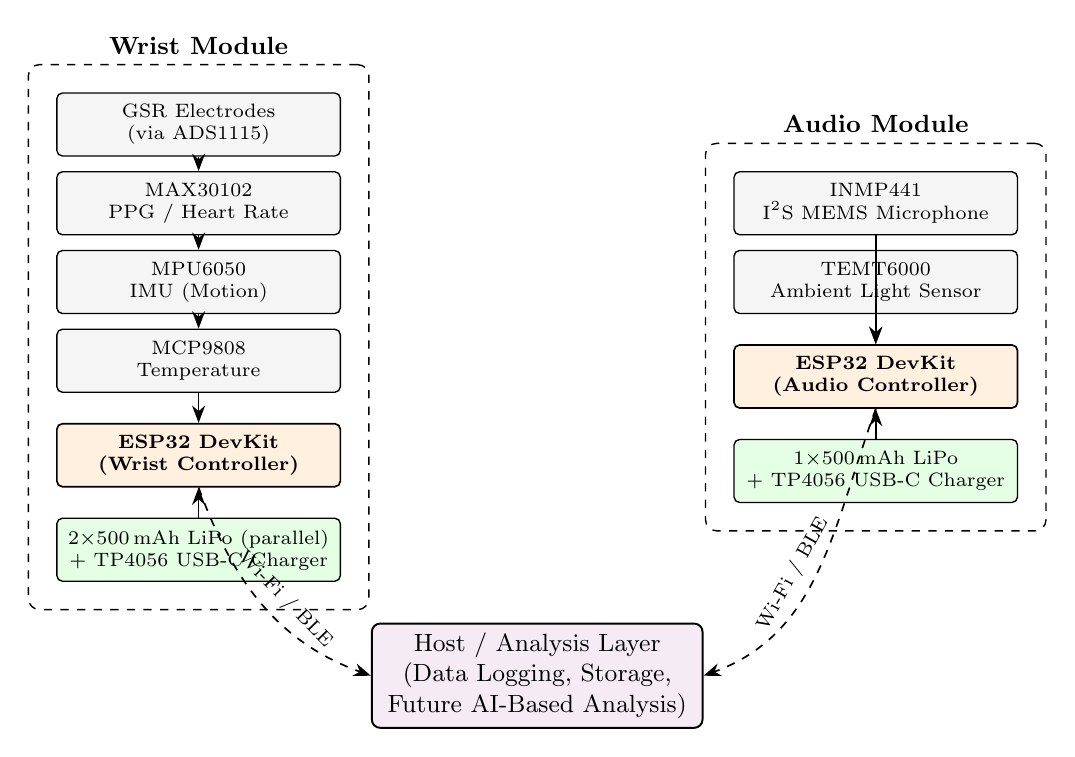
\begin{tikzpicture}[
    font=\small,
    module/.style={draw, rounded corners=3pt, fill=blue!6, minimum width=4.6cm, minimum height=1cm, align=center, line width=0.6pt},
    sensor/.style={draw, rounded corners=2pt, fill=gray!8, minimum width=3.6cm, minimum height=0.8cm, align=center, line width=0.5pt, font=\scriptsize},
    ctrl/.style={draw, rounded corners=2pt, fill=orange!12, minimum width=3.6cm, minimum height=0.8cm, align=center, line width=0.6pt, font=\scriptsize\bfseries},
    pwr/.style={draw, rounded corners=2pt, fill=green!10, minimum width=3.6cm, minimum height=0.8cm, align=center, line width=0.5pt, font=\scriptsize},
    host/.style={draw, rounded corners=3pt, fill=violet!8, minimum width=4.2cm, minimum height=1.2cm, align=center, line width=0.7pt},
    arrow/.style={-{Stealth[length=2.2mm]}, line width=0.6pt},
    dashedbox/.style={draw, dashed, rounded corners=4pt, inner sep=10pt, line width=0.5pt}
]

% ---- Wrist Module cluster ----
\node[sensor] (gsr) at (0,6.4) {GSR Electrodes\\(via ADS1115)};
\node[sensor] (max30102) at (0,5.4) {MAX30102\\PPG / Heart Rate};
\node[sensor] (mpu6050) at (0,4.4) {MPU6050\\IMU (Motion)};
\node[sensor] (mcp9808) at (0,3.4) {MCP9808\\Temperature};
\node[ctrl] (esp32wrist) at (0,2.2) {ESP32 DevKit\\(Wrist Controller)};
\node[pwr] (pwrwrist) at (0,1.0) {2$\times$500\,mAh LiPo (parallel)\\+ TP4056 USB-C Charger};

\node[dashedbox, fit=(gsr)(max30102)(mpu6050)(mcp9808)(esp32wrist)(pwrwrist), label={[font=\bfseries\small]above:Wrist Module}] (wristbox) {};

% ---- Audio Module cluster ----
\node[sensor] (mic) at (8.6,5.4) {INMP441\\I\textsuperscript{2}S MEMS Microphone};
\node[sensor] (light) at (8.6,4.4) {TEMT6000\\Ambient Light Sensor};
\node[ctrl] (esp32audio) at (8.6,3.2) {ESP32 DevKit\\(Audio Controller)};
\node[pwr] (pwraudio) at (8.6,2.0) {1$\times$500\,mAh LiPo\\+ TP4056 USB-C Charger};

\node[dashedbox, fit=(mic)(light)(esp32audio)(pwraudio), label={[font=\bfseries\small]above:Audio Module}] (audiobox) {};

% ---- Host / analysis layer ----
\node[host] (host) at (4.3,-0.6) {Host / Analysis Layer\\(Data Logging, Storage,\\Future AI-Based Analysis)};

% ---- Internal connections: Wrist Module ----
\draw[arrow] (gsr.south) -- (max30102.north);
\draw[arrow] (max30102.south) -- (mpu6050.north);
\draw[arrow] (mpu6050.south) -- (mcp9808.north);
\draw[arrow] (mcp9808.south) -- (esp32wrist.north);
\draw[arrow] (pwrwrist.north) -- (esp32wrist.south);

% ---- Internal connections: Audio Module ----
\draw[arrow] (mic.south) -- (esp32audio.north);
\draw[arrow] (light.south) -- (esp32audio.north);
\draw[arrow] (pwraudio.north) -- (esp32audio.south);

% ---- Wireless links to host ----
\draw[arrow, dashed] (esp32wrist.south) to[out=-70,in=160] node[pos=0.55, above, sloped, font=\scriptsize]{Wi-Fi / BLE} (host.west);
\draw[arrow, dashed] (esp32audio.south) to[out=-110,in=20] node[pos=0.55, above, sloped, font=\scriptsize]{Wi-Fi / BLE} (host.east);

\end{tikzpicture}
\caption{High-level system architecture of PSYCON, showing the Wrist Module (physiological sensing) and Audio Module (speech and environmental sensing) as independently powered ESP32-based subsystems that communicate wirelessly with a host/analysis layer.}
\label{fig:system-architecture}
\end{figure*}

\subsubsection{Wrist Module}
\label{sec:wrist-module}

\textbf{Purpose.} Physiological data acquisition.

\textbf{Sensors.}
\begin{itemize}
    \item GSR electrodes (via ADS1115)
    \item MAX30102 pulse oximeter / heart-rate sensor
    \item MPU6050 inertial measurement unit
    \item MCP9808 digital temperature sensor
\end{itemize}

\textbf{Controller.} ESP32 DevKit (30-pin).

\textbf{Power.} Two 500\,mAh LiPo batteries connected in parallel ($\approx$1000\,mAh total capacity), charged and protected via a TP4056 USB-C charging module.

\subsubsection{Audio Module}
\label{sec:audio-module}

\textbf{Purpose.} Speech acquisition and environmental sensing.

\textbf{Sensors.}
\begin{itemize}
    \item INMP441 I\textsuperscript{2}S MEMS microphone
    \item TEMT6000 ambient light sensor
\end{itemize}

\textbf{Controller.} ESP32 DevKit (30-pin).

\textbf{Power.} One 500\,mAh LiPo battery, charged and protected via a TP4056 USB-C charging module.

\subsection{Data Collected}
\label{sec:data-collected}

\Cref{tab:data-collected} summarizes the categories of data acquired by PSYCON across its two modules.

\begin{table}[H]
\centering
\caption{Data modalities collected by PSYCON.}
\label{tab:data-collected}
\small
\begin{tabularx}{\columnwidth}{@{}l Y@{}}
\toprule
\textbf{Category} & \textbf{Signals / Data} \\
\midrule
Physiological & Heart rate; pulse waveform (PPG); skin conductance (EDA/GSR); skin temperature; motion and orientation \\
Environmental & Ambient light level \\
Audio & Speech recordings for future AI feature extraction \\
\bottomrule
\end{tabularx}
\end{table}

\subsection{Design Philosophy}
\label{sec:design-philosophy}

The system follows five core engineering principles:

\begin{itemize}
    \item \textbf{Modularity} --- each subsystem can operate and be tested independently.
    \item \textbf{Scalability} --- prototype hardware should transition cleanly to a custom PCB.
    \item \textbf{Maintainability} --- use widely available, well-documented modules.
    \item \textbf{Low Cost} --- balance performance with affordability.
    \item \textbf{Research Focus} --- prioritize data quality and documentation over product miniaturization.
\end{itemize}

\subsection{Current Hardware Configuration}
\label{sec:current-hardware-configuration}

\Cref{tab:hardware-config} summarizes the current bill-of-materials-level hardware configuration for the PSYCON prototype, organized by controllers, power components, and sensors.

\begin{table}[H]
\centering
\caption{Current hardware configuration of the PSYCON prototype.}
\label{tab:hardware-config}
\small
\begin{tabularx}{\columnwidth}{@{}l Y c@{}}
\toprule
\textbf{Category} & \textbf{Component} & \textbf{Qty.} \\
\midrule
Controllers & ESP32 DevKit (30-pin) & 2 \\
\midrule
\multirow{2}{*}{Power} & TP4056 USB-C charger module (protected) & 2 \\
 & 500\,mAh 3.7\,V LiPo battery (HLCY 651735P) & 3 \\
\midrule
\multirow{6}{*}{Sensors} & MAX30102 pulse oximeter / heart-rate sensor & 1 \\
 & ADS1115 16-bit ADC & 1 \\
 & MPU6050 IMU & 1 \\
 & MCP9808 temperature sensor & 1 \\
 & TEMT6000 ambient light sensor & 1 \\
 & INMP441 I\textsuperscript{2}S MEMS microphone & 1 \\
 & GSR electrodes (analog front end TBD) & 1 set \\
\bottomrule
\end{tabularx}
\end{table}

\subsection{Communication Interfaces}
\label{sec:communication-interfaces}

\Cref{tab:comm-interfaces} lists the communication interfaces used to connect each sensor to its respective ESP32 controller.

\begin{table}[H]
\centering
\caption{Communication interfaces by sensor.}
\label{tab:comm-interfaces}
\small
\begin{tabularx}{\columnwidth}{@{}l Y@{}}
\toprule
\textbf{Interface} & \textbf{Connected Devices} \\
\midrule
I\textsuperscript{2}C & MAX30102, MPU6050, ADS1115, MCP9808 \\
I\textsuperscript{2}S & INMP441 \\
Analog & TEMT6000; GSR electrodes (through ADS1115) \\
Wi-Fi / BLE & ESP32 wireless communication (both modules) \\
\bottomrule
\end{tabularx}
\end{table}

\subsection{Engineering Status}
\label{sec:engineering-status}

\begin{validationbox}
\textbf{Confirmed:}
\begin{itemize}
    \item Component selection
    \item Module compatibility
    \item I\textsuperscript{2}C address compatibility
    \item Overall system architecture
    \item Power subsystem concept
    \item Sensor allocation between modules
\end{itemize}
\end{validationbox}

\begin{requirementbox}
\textbf{Pending validation:}
\begin{itemize}
    \item Final GSR analog front end
    \item Full firmware integration
    \item Electrical characterization (current, runtime, thermal)
    \item Long-duration testing
\end{itemize}
\end{requirementbox}

\subsection{Assumptions and Scope}
\label{sec:assumptions-scope}

This document distinguishes between three categories of technical claims:

\begin{itemize}
    \item \textbf{Confirmed information} --- derived from hardware, datasheets, and documented design decisions.
    \item \textbf{Engineering assumptions} --- based on standard module implementations.
    \item \textbf{Experimental items} --- items that require physical testing before they can be claimed as verified.
\end{itemize}

\begin{assumptionbox}
The distinction above is maintained throughout this document to preserve technical accuracy suitable for engineering documentation and science-competition review. Where a claim has not yet been experimentally validated, it is explicitly flagged rather than presented as a confirmed result.
\end{assumptionbox}


% ============================================================
% CHAPTER 2
% ============================================================
% ============================================================
% Chapter 2 — System Requirements Specification (SRS)
% Source: PSYCON Engineering Design Document, Vol. 1, Ch. 2
% ============================================================
\section{System Requirements Specification}
\label{sec:srs}

\subsection{Purpose}
\label{sec:srs-purpose}

This section defines exactly what PSYCON is expected to do from an engineering perspective. The requirements stated here act as the baseline against which the prototype will be evaluated.

\subsection{Design Objectives}
\label{sec:design-objectives}

The system shall:
\begin{itemize}
    \item Continuously collect physiological data.
    \item Continuously collect speech samples.
    \item Continuously monitor environmental conditions.
    \item Synchronize all collected data.
    \item Operate as a wearable prototype.
    \item Be modular.
    \item Be expandable.
    \item Be low-cost.
    \item Be reproducible using commercially available components.
    \item Support future AI-based analysis.
\end{itemize}

\subsection{Functional Requirements}
\label{sec:functional-requirements}

\subsubsection{FR-1: Physiological Monitoring}
The wrist module shall measure heart rate, pulse waveform (PPG), skin conductance (EDA/GSR), skin temperature, wrist motion, and wrist orientation.

\noindent\textit{Status:} \doneTag\ Hardware selected \quad \pendingTag\ Integration pending

\subsubsection{FR-2: Audio Monitoring}
The audio module shall capture speech, digitize audio using I\textsuperscript{2}S, stream or store recordings, and maintain synchronized timestamps.

\noindent\textit{Status:} \doneTag\ Hardware selected \quad \pendingTag\ Firmware pending

\subsubsection{FR-3: Environmental Monitoring}
The system shall measure ambient light for purposes of context awareness, sleep/environment correlation, and future feature extraction.

\noindent\textit{Status:} \doneTag\ Hardware selected

\subsubsection{FR-4: Data Synchronization}
The system shall timestamp every sample, preserve acquisition order, and allow synchronization between the wrist and audio modules. This requirement is critical because machine-learning analysis becomes unreliable if physiological and audio events are misaligned in time.

\noindent\textit{Status:} \pendingTag\ Firmware requirement

\subsubsection{FR-5: Wireless Communication}
Each ESP32 shall support Wi-Fi and BLE (future expansion), enabling data upload, remote monitoring, over-the-air (OTA) firmware updates (future), and local communication.

\noindent\textit{Status:} \doneTag\ Supported by hardware

\subsubsection{FR-6: Local Processing}
Each module shall read sensors, filter signals, package data, detect sensor failures, and continue operation independently of the other module.

\subsubsection{FR-7: Modular Operation}
If one module fails, the second module shall continue operating. For example, an audio-module failure shall not stop physiological acquisition, and a physiological-module failure shall not stop audio acquisition.

\subsubsection{FR-8: Expandability}
Future sensors should be addable without redesigning the architecture. Candidate future sensors include ECG, EEG, EMG, respiration, skin hydration, and air-quality sensing.

\subsection{Non-Functional Requirements}
\label{sec:non-functional-requirements}

\textbf{Reliability.} The target is continuous operation without crashes. The prototype goal is a minimum continuous runtime of 6\,h, with a stretch goal of 24\,h.

\textbf{Accuracy.} Sensors should operate within manufacturer specifications; no artificial software correction should replace proper calibration.

\textbf{Repeatability.} Repeated measurements under identical conditions should produce similar results, which is especially important for GSR, heart rate, and temperature.

\textbf{Maintainability.} The system should use standard breakout boards, use labeled connectors, allow module replacement, and support firmware updates.

\textbf{Portability.} The system should fit on the body, operate on batteries, and avoid wired external power during use.

\textbf{Scalability.} Future revisions should migrate easily to a custom PCB, smaller ESP32 variants, and improved analog front ends.

\textbf{Cost.} The primary objective is high capability with affordable hardware; the approximate prototype cost target is lower than research-grade commercial systems.

\textbf{Safety.} The wearable shall use protected LiPo batteries, avoid exposed battery terminals, maintain a safe GSR excitation current, avoid charging while connected to GSR electrodes, and use insulated wiring.

\subsection{Performance Targets}
\label{sec:performance-targets}

\Cref{tab:performance-targets} summarizes the target operating behavior for each monitored parameter.

\begin{table}[H]
\centering
\caption{Performance targets by parameter.}
\label{tab:performance-targets}
\small
\begin{tabularx}{\columnwidth}{@{}Y l@{}}
\toprule
\textbf{Parameter} & \textbf{Target} \\
\midrule
Heart-rate monitoring & Continuous \\
GSR monitoring & Continuous \\
Temperature monitoring & Continuous \\
Motion monitoring & Continuous \\
Ambient light & Continuous \\
Speech recording & Continuous or scheduled \\
Wireless communication & Stable \\
Battery-powered & Yes \\
Rechargeable & Yes \\
\bottomrule
\end{tabularx}
\end{table}

\subsection{Hardware Constraints}
\label{sec:hardware-constraints}

\Cref{tab:hardware-constraints} lists the hardware constraints of the finalized design, organized by controllers, power, and sensor allocation between the wrist and audio modules.

\begin{table}[H]
\centering
\caption{Hardware constraints of the finalized PSYCON design.}
\label{tab:hardware-constraints}
\small
\begin{tabularx}{\columnwidth}{@{}l Y@{}}
\toprule
\textbf{Category} & \textbf{Components} \\
\midrule
Controllers & 2 $\times$ ESP32 DevKit (30-pin) \\
Power & 2 $\times$ TP4056 USB-C charger; 3 $\times$ 500\,mAh LiPo battery \\
Wrist sensors & MAX30102; ADS1115; MCP9808; MPU6050; GSR electrodes \\
Audio sensors & INMP441; TEMT6000 \\
\bottomrule
\end{tabularx}
\end{table}

\subsection{Software Constraints}
\label{sec:software-constraints}

Firmware should:
\begin{itemize}
    \item Support FreeRTOS tasks (recommended).
    \item Prevent blocking sensor reads.
    \item Handle communication failures gracefully.
    \item Log errors.
    \item Support firmware expansion.
\end{itemize}

\subsection{Data Requirements}
\label{sec:data-requirements}

Every record should include a timestamp, module ID, sensor ID, sensor values, battery level (future), and error flags (future). \Cref{fig:data-record-flow} illustrates the logical structure of a single data record as it is composed prior to storage or transmission.

\begin{figure}[H]
\centering
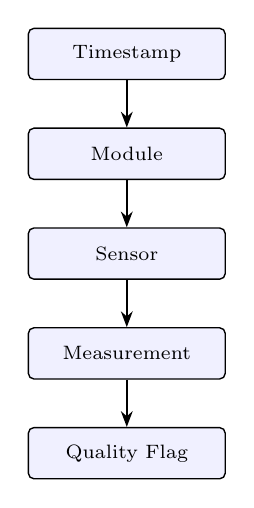
\begin{tikzpicture}[
    font=\scriptsize,
    node distance=0mm,
    field/.style={draw, rounded corners=2pt, fill=blue!6, minimum width=2.5cm, minimum height=0.65cm, align=center, line width=0.5pt}
]
\node[field] (ts) {Timestamp};
\node[field, below=6mm of ts] (mod) {Module};
\node[field, below=6mm of mod] (sen) {Sensor};
\node[field, below=6mm of sen] (meas) {Measurement};
\node[field, below=6mm of meas] (qf) {Quality Flag};

\draw[-{Stealth[length=2mm]}, line width=0.6pt] (ts.south) -- (mod.north);
\draw[-{Stealth[length=2mm]}, line width=0.6pt] (mod.south) -- (sen.north);
\draw[-{Stealth[length=2mm]}, line width=0.6pt] (sen.south) -- (meas.north);
\draw[-{Stealth[length=2mm]}, line width=0.6pt] (meas.south) -- (qf.north);
\end{tikzpicture}
\caption{Logical structure of a single PSYCON data record, composed sequentially from acquisition timestamp through to a quality flag.}
\label{fig:data-record-flow}
\end{figure}

\subsection{Assumptions}
\label{sec:srs-assumptions}

\begin{assumptionbox}
The following are treated as current engineering assumptions until experimentally verified:
\begin{itemize}
    \item Standard module revisions.
    \item Standard operating voltages.
    \item No I\textsuperscript{2}C address conflicts.
    \item Proper power distribution.
    \item Common ground maintained.
    \item Standard ESP32 DevKit V1 behavior.
\end{itemize}
\end{assumptionbox}

\subsection{Risks}
\label{sec:risks}

\Cref{tab:risks} summarizes known engineering risks by priority level.

\begin{table}[H]
\centering
\caption{Known engineering risks by priority.}
\label{tab:risks}
\small
\begin{tabularx}{\columnwidth}{@{}l Y@{}}
\toprule
\textbf{Priority} & \textbf{Risk} \\
\midrule
\highriskTag & GSR analog front-end quality \\
\highriskTag & Battery runtime \\
\highriskTag & Charging while operating \\
\highriskTag & Long-term stability \\
\midrule
\medriskTag & Audio noise \\
\medriskTag & Motion artifacts \\
\medriskTag & Synchronization drift \\
\midrule
\lowriskTag & I\textsuperscript{2}C conflicts (none expected) \\
\lowriskTag & GPIO availability \\
\lowriskTag & Sensor compatibility \\
\bottomrule
\end{tabularx}
\end{table}

\subsection{Acceptance Criteria}
\label{sec:acceptance-criteria}

The prototype is considered functionally complete when:
\begin{itemize}
    \item All sensors initialize successfully.
    \item No I\textsuperscript{2}C address conflicts occur.
    \item Audio records correctly.
    \item Physiological data streams continuously.
    \item Modules operate independently.
    \item Battery operation is stable.
    \item Data timestamps remain synchronized.
    \item Documentation is complete.
    \item Safety procedures are documented.
    \item Hardware passes integration testing.
\end{itemize}

\subsection{Chapter Status}
\label{sec:ch2-status}

\begin{validationbox}
\textbf{Completed for this chapter:}
\begin{itemize}
    \item Functional requirements
    \item Non-functional requirements
    \item Design objectives
    \item Constraints (hardware and software)
    \item Acceptance criteria
    \item Risk overview
    \item Data requirements
\end{itemize}
\end{validationbox}


% ============================================================
% CHAPTER 3
% ============================================================
% ============================================================
% Chapter 3 — Overall System Architecture
% Source: PSYCON Engineering Design Document, Vol. 1, Ch. 3
% ============================================================
\section{Overall System Architecture}
\label{sec:overall-architecture}

\subsection{System Overview}
\label{sec:system-overview}

PSYCON is a distributed wearable sensing platform consisting of two independent electronic modules that work together to collect synchronized multimodal data for psychological state analysis. The architecture intentionally separates physiological sensing from speech sensing to reduce electrical noise, improve wearability, simplify mechanical design, and allow each subsystem to operate independently.

\subsection{High-Level Architecture}
\label{sec:high-level-architecture-ch3}

\Cref{fig:top-level-pipeline} presents the top-level data pipeline of PSYCON, from the two physical modules through synchronization, AI processing, and final psychological-condition assessment.

\begin{figure*}[t]
\centering
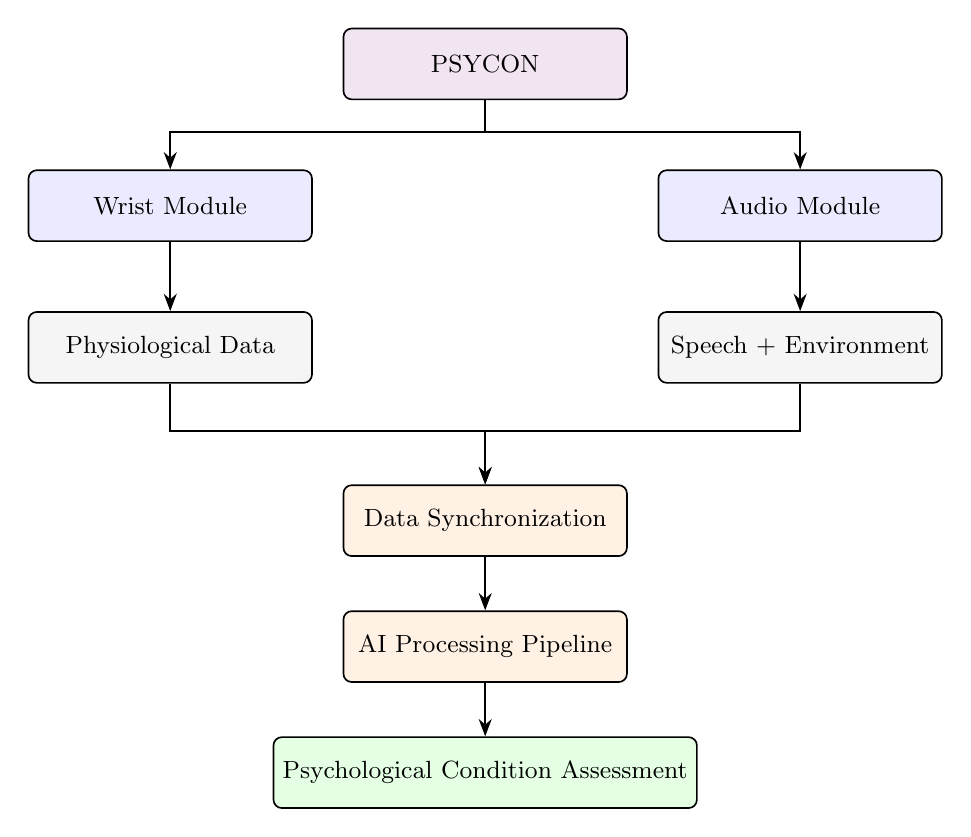
\begin{tikzpicture}[
    font=\small,
    stage/.style={draw, rounded corners=3pt, minimum width=3.6cm, minimum height=0.9cm, align=center, line width=0.6pt},
    top/.style={stage, fill=violet!10},
    mod/.style={stage, fill=blue!8},
    data/.style={stage, fill=gray!8},
    proc/.style={stage, fill=orange!10},
    result/.style={stage, fill=green!10},
    arrow/.style={-{Stealth[length=2.2mm]}, line width=0.6pt}
]

\node[top] (psycon) at (6,9.6) {PSYCON};

\node[mod] (wrist) at (2,7.8) {Wrist Module};
\node[mod] (audio) at (10,7.8) {Audio Module};

\node[data] (phys) at (2,6.0) {Physiological Data};
\node[data] (speech) at (10,6.0) {Speech + Environment};

\node[proc] (sync) at (6,3.8) {Data Synchronization};
\node[proc] (ai) at (6,2.2) {AI Processing Pipeline};
\node[result] (assess) at (6,0.6) {Psychological Condition Assessment};

\draw[arrow] (psycon.south) -- ++(0,-4mm) -| (wrist.north);
\draw[arrow] (psycon.south) -- ++(0,-4mm) -| (audio.north);
\draw[arrow] (wrist.south) -- (phys.north);
\draw[arrow] (audio.south) -- (speech.north);
\draw[arrow] (phys.south) -- ++(0,-6mm) -| (sync.north);
\draw[arrow] (speech.south) -- ++(0,-6mm) -| (sync.north);
\draw[arrow] (sync.south) -- (ai.north);
\draw[arrow] (ai.south) -- (assess.north);

\end{tikzpicture}
\caption{Top-level PSYCON data pipeline: independent acquisition by the Wrist and Audio Modules, followed by data synchronization, AI processing, and psychological-condition assessment.}
\label{fig:top-level-pipeline}
\end{figure*}

\subsection{Module Responsibilities}
\label{sec:module-responsibilities}

\subsubsection{Wrist Module}
\textbf{Purpose.} Collect physiological signals directly from the user's body.

\textbf{Primary functions.}
\begin{itemize}
    \item Heart-rate monitoring
    \item Pulse waveform acquisition
    \item Electrodermal activity (GSR)
    \item Skin temperature
    \item Motion sensing
    \item Timestamp generation
    \item Wireless communication
\end{itemize}

\subsubsection{Audio Module}
\textbf{Purpose.} Collect speech and environmental context.

\textbf{Primary functions.}
\begin{itemize}
    \item Speech recording
    \item Ambient light monitoring
    \item Timestamp generation
    \item Wireless communication
\end{itemize}

\subsection{Wrist Module Hardware}
\label{sec:wrist-module-hardware}

\textbf{Controller.} ESP32 DevKit (30-pin). Responsibilities include reading all sensors, managing I\textsuperscript{2}C communication, processing sensor data, buffering measurements, transmitting data, and managing power state.

\textbf{MAX30102.} Measures heart rate and pulse waveform (PPG) over an I\textsuperscript{2}C interface.

\textbf{ADS1115.} Provides high-resolution analog-to-digital conversion and is connected to the GSR analog front end.

\begin{designnote}
The ESP32's internal ADC has limited precision and non-linearity. The ADS1115 provides a 16-bit ADC with programmable gain, making it more suitable for low-level analog measurements such as GSR.
\end{designnote}

\textbf{GSR electrodes.} Measure changes in skin conductance associated with sweat-gland activity.

\begin{requirementbox}
\textbf{Current status:} electrodes selected; the analog front end is to be finalized and validated before human testing.
\end{requirementbox}

\textbf{MPU6050.} Measures acceleration and angular velocity, used for motion detection, activity recognition, and motion-artifact identification.

\textbf{MCP9808.} Measures skin temperature.

\begin{designnote}
The MCP9808 was selected because it provides higher accuracy and stability than common low-cost temperature sensors.
\end{designnote}

\subsection{Audio Module Hardware}
\label{sec:audio-module-hardware}

\textbf{Controller.} ESP32 DevKit (30-pin). Responsibilities include reading the microphone, reading the ambient light sensor, timestamping audio, and managing wireless communication.

\textbf{INMP441.} Measures digital audio over an I\textsuperscript{2}S interface and is used for speech feature extraction, voice-quality analysis, and future AI models.

\textbf{TEMT6000.} Measures ambient light intensity and is used for environmental context, sleep and activity correlation, and context-aware analysis.

\subsection{Power Architecture}
\label{sec:power-architecture}

Each module operates independently, with its own battery, charging/protection circuit, and regulated rail. \Cref{fig:power-architecture} shows the power chain for both modules side by side.

\begin{figure*}[t]
\centering
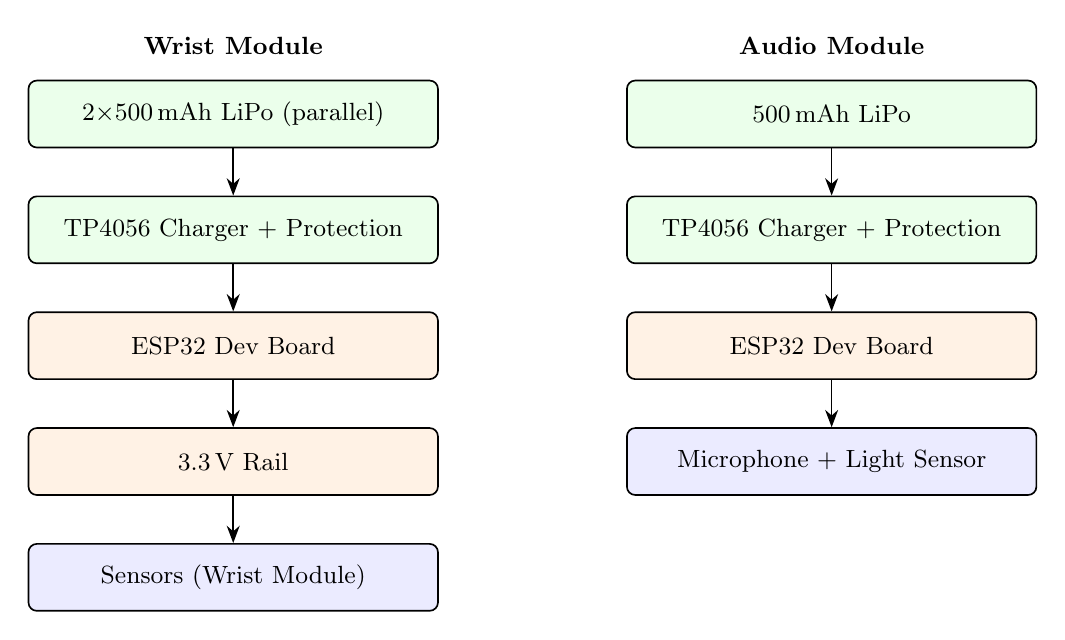
\begin{tikzpicture}[
    font=\small,
    pwrstage/.style={draw, rounded corners=3pt, minimum width=5.2cm, minimum height=0.85cm, align=center, line width=0.6pt, fill=green!8},
    ctrlstage/.style={draw, rounded corners=3pt, minimum width=5.2cm, minimum height=0.85cm, align=center, line width=0.6pt, fill=orange!10},
    loadstage/.style={draw, rounded corners=3pt, minimum width=5.2cm, minimum height=0.85cm, align=center, line width=0.6pt, fill=blue!8},
    arrow/.style={-{Stealth[length=2.2mm]}, line width=0.6pt}
]

% Wrist Module power chain
\node[pwrstage] (w1) at (0,4) {2$\times$500\,mAh LiPo (parallel)};
\node[pwrstage, below=6mm of w1] (w2) {TP4056 Charger + Protection};
\node[ctrlstage, below=6mm of w2] (w3) {ESP32 Dev Board};
\node[ctrlstage, below=6mm of w3] (w4) {3.3\,V Rail};
\node[loadstage, below=6mm of w4] (w5) {Sensors (Wrist Module)};

\draw[arrow] (w1.south) -- (w2.north);
\draw[arrow] (w2.south) -- (w3.north);
\draw[arrow] (w3.south) -- (w4.north);
\draw[arrow] (w4.south) -- (w5.north);

\node[above=2mm of w1, font=\bfseries\small] {Wrist Module};

% Audio Module power chain
\node[pwrstage] (a1) at (7.6,4) {500\,mAh LiPo};
\node[pwrstage, below=6mm of a1] (a2) {TP4056 Charger + Protection};
\node[ctrlstage, below=6mm of a2] (a3) {ESP32 Dev Board};
\node[loadstage, below=6mm of a3] (a4) {Microphone + Light Sensor};

\draw[arrow] (a1.south) -- (a2.north);
\draw[arrow] (a2.south) -- (a3.north);
\draw[arrow] (a3.south) -- (a4.north);

\node[above=2mm of a1, font=\bfseries\small] {Audio Module};

\end{tikzpicture}
\caption{Independent power architecture for the Wrist Module (estimated battery capacity $\approx$1000\,mAh) and the Audio Module, each with dedicated LiPo battery, TP4056 charge/protection circuit, and ESP32 controller.}
\label{fig:power-architecture}
\end{figure*}

The Wrist Module's parallel two-cell configuration yields an estimated battery capacity of approximately 1000\,mAh, while the Audio Module operates from a single 500\,mAh cell.

\subsection{Communication Architecture}
\label{sec:communication-architecture-ch3}

\subsubsection{I\texorpdfstring{\textsuperscript{2}}{2}C Bus (Wrist Module)}
The I\textsuperscript{2}C bus on the Wrist Module is shared by the MAX30102, ADS1115, MCP9808, and MPU6050. \Cref{tab:i2c-addresses} lists the expected device addresses; no address conflicts are expected.

\begin{table}[H]
\centering
\caption{Expected I\textsuperscript{2}C device addresses on the Wrist Module bus.}
\label{tab:i2c-addresses}
\small
\begin{tabularx}{\columnwidth}{@{}Y l@{}}
\toprule
\textbf{Device} & \textbf{Address} \\
\midrule
MCP9808 & \texttt{0x18} \\
ADS1115 & \texttt{0x48} \\
MAX30102 & \texttt{0x57} \\
MPU6050 & \texttt{0x68} (default) \\
\bottomrule
\end{tabularx}
\end{table}

\subsubsection{I\texorpdfstring{\textsuperscript{2}}{2}S Bus (Audio Module)}
The I\textsuperscript{2}S bus connects the INMP441 microphone and carries the bit clock (SCK/BCLK), word select (WS/LRCLK), and serial data (SD) signals.

\subsubsection{Analog Signals}
Analog signals are handled through the ADS1115, including the GSR analog output. The TEMT6000 provides an analog output that may be connected either to an ESP32 ADC pin or to an ADS1115 channel if higher measurement precision is desired.

\subsection{Data Flow}
\label{sec:data-flow}

\Cref{fig:data-flow-pipeline} shows the end-to-end data flow from sensor acquisition through to AI processing. Each sample should receive its timestamp as close to acquisition as possible to minimize synchronization errors.

\begin{figure*}[t]
\centering
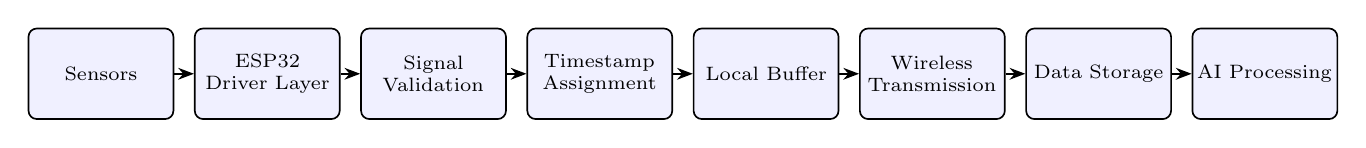
\begin{tikzpicture}[
    font=\scriptsize,
    stage/.style={draw, rounded corners=3pt, text width=1.7cm, minimum height=1.15cm, align=center, line width=0.6pt, fill=blue!6, inner sep=2pt},
    arrow/.style={-{Stealth[length=2mm]}, line width=0.6pt},
    node distance=2.5mm
]
\node[stage] (s1) {Sensors};
\node[stage, right=of s1] (s2) {ESP32 Driver Layer};
\node[stage, right=of s2] (s3) {Signal Validation};
\node[stage, right=of s3] (s4) {Timestamp Assignment};
\node[stage, right=of s4] (s5) {Local Buffer};
\node[stage, right=of s5] (s6) {Wireless Transmission};
\node[stage, right=of s6] (s7) {Data Storage};
\node[stage, right=of s7] (s8) {AI Processing};

\foreach \i/\j in {s1/s2, s2/s3, s3/s4, s4/s5, s5/s6, s6/s7, s7/s8}
  \draw[arrow] (\i.east) -- (\j.west);
\end{tikzpicture}
\caption{End-to-end PSYCON data flow, from raw sensor acquisition through driver-level reads, validation, timestamping, buffering, wireless transmission, storage, and AI processing.}
\label{fig:data-flow-pipeline}
\end{figure*}

\subsection{Power Flow}
\label{sec:power-flow}

\Cref{fig:power-flow} shows the generic power flow within each module, from battery through to the sensor loads. All sensors share a common ground within their respective module.

\begin{figure}[H]
\centering
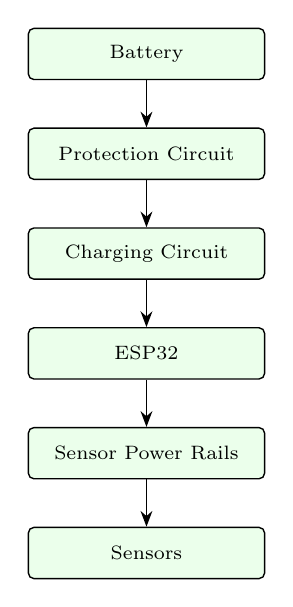
\begin{tikzpicture}[
    font=\scriptsize,
    node distance=0mm,
    field/.style={draw, rounded corners=2pt, fill=green!8, minimum width=3.0cm, minimum height=0.65cm, align=center, line width=0.5pt}
]
\node[field] (bat) {Battery};
\node[field, below=6mm of bat] (prot) {Protection Circuit};
\node[field, below=6mm of prot] (chg) {Charging Circuit};
\node[field, below=6mm of chg] (mcu) {ESP32};
\node[field, below=6mm of mcu] (rail) {Sensor Power Rails};
\node[field, below=6mm of rail] (sens) {Sensors};

\draw[-{Stealth[length=2mm]}, line width=0.6pt] (bat.south) -- (prot.north);
\draw[-{Stealth[length=2mm]}, line width=0.6pt] (prot.south) -- (chg.north);
\draw[-{Stealth[length=2mm]}, line width=0.6pt] (chg.south) -- (mcu.north);
\draw[-{Stealth[length=2mm]}, line width=0.6pt] (mcu.south) -- (rail.north);
\draw[-{Stealth[length=2mm]}, line width=0.6pt] (rail.south) -- (sens.north);
\end{tikzpicture}
\caption{Generic per-module power flow, from battery through protection and charging circuitry to the microcontroller and sensor power rails.}
\label{fig:power-flow}
\end{figure}

\subsection{Synchronization Strategy}
\label{sec:synchronization-strategy}

Although physically separate, both modules should:
\begin{itemize}
    \item Use a consistent time base.
    \item Include timestamps with every data packet.
    \item Include a module identifier.
    \item Include sensor identifiers.
    \item Handle temporary communication interruptions without losing acquisition order.
\end{itemize}

\subsection{Fault Isolation}
\label{sec:fault-isolation}

A failure in one module should not prevent the other from operating. For example, if the microphone fails, physiological sensing continues; if the wrist module resets, audio acquisition continues; and if wireless communication is unavailable, data should be buffered, subject to firmware support.

\subsection{Engineering Advantages of the Split Architecture}
\label{sec:split-architecture-advantages}

\begin{observationbox}
\begin{itemize}
    \item Reduced electrical interference between analog sensors and the microphone.
    \item Better weight distribution for wearability.
    \item Simpler wiring within each module.
    \item Independent testing and debugging.
    \item Easier future upgrades or PCB redesigns.
    \item Greater fault tolerance.
\end{itemize}
\end{observationbox}

\subsection{Current Limitations}
\label{sec:current-limitations-ch3}

\begin{requirementbox}
\textbf{The following items remain to be validated experimentally:}
\begin{itemize}
    \item Final GSR analog front-end implementation.
    \item Battery runtime under real workloads.
    \item Continuous-operation stability.
    \item Thermal behavior during charging and prolonged operation.
    \item Wireless throughput and latency under sustained use.
    \item Long-term synchronization accuracy.
\end{itemize}
\end{requirementbox}

\subsection{Chapter Status}
\label{sec:ch3-status}

\begin{validationbox}
\textbf{Completed for this chapter:}
\begin{itemize}
    \item Overall system architecture
    \item Module separation rationale
    \item Hardware block architecture
    \item Data flow
    \item Power flow
    \item Communication architecture
    \item Synchronization strategy
    \item Fault isolation
    \item Engineering design rationale
    \item Current limitations
\end{itemize}
\end{validationbox}


% ============================================================
% CHAPTER 4
% ============================================================
% ============================================================
% Chapter 4 — Complete Hardware Design
% Source: PSYCON Engineering Design Document, Vol. 1, Ch. 4
% ============================================================
\section{Complete Hardware Design}
\label{sec:hardware-design}

\subsection{Hardware Design Philosophy}
\label{sec:hardware-design-philosophy}

The hardware platform was designed with the following priorities:
\begin{itemize}
    \item Research-grade sensor selection within a student budget.
    \item Modular architecture for independent testing.
    \item Commercially available components.
    \item Easy replacement and maintenance.
    \item Future migration to a custom PCB.
    \item Low-voltage battery-powered operation.
    \item Standard communication protocols (I\textsuperscript{2}C, I\textsuperscript{2}S, ADC).
\end{itemize}

\subsection{Complete Bill of Hardware}
\label{sec:bill-of-hardware}

\Cref{tab:bill-of-hardware} lists the complete hardware inventory for the PSYCON prototype, including quantity, module assignment, and function of each component.

\begin{table*}[t]
\centering
\caption{Complete bill of hardware for the PSYCON prototype.}
\label{tab:bill-of-hardware}
\small
\begin{tabularx}{\textwidth}{@{}Y c l Y@{}}
\toprule
\textbf{Component} & \textbf{Qty.} & \textbf{Module} & \textbf{Function} \\
\midrule
ESP32 DevKit (30-pin) & 2 & Both & Main controller \\
TP4056 USB-C charger (HW-373 V1.2.1, protected) & 2 & Both & Battery charging and protection \\
500\,mAh 3.7\,V LiPo (HLCY 651735P) & 3 & Both & Power source \\
MAX30102 & 1 & Wrist & Heart rate \& PPG \\
ADS1115 & 1 & Wrist & 16-bit ADC \\
GSR electrodes & 1 pair & Wrist & Skin conductance \\
MPU6050 & 1 & Wrist & Motion sensing \\
MCP9808 & 1 & Wrist & Temperature \\
INMP441 & 1 & Audio & Digital microphone \\
TEMT6000 & 1 & Audio & Ambient light \\
\bottomrule
\end{tabularx}
\end{table*}

\subsection{ESP32 DevKit (30-pin)}
\label{sec:esp32-devkit}

\textbf{Role.} Primary microcontroller responsible for sensor acquisition, data processing, wireless communication, timestamp generation, power management, and firmware execution.

\Cref{tab:esp32-specs} lists the key specifications of the ESP32 DevKit.

\begin{table}[H]
\centering
\caption{Key specifications of the ESP32 DevKit (30-pin).}
\label{tab:esp32-specs}
\small
\begin{tabularx}{\columnwidth}{@{}l Y@{}}
\toprule
\textbf{Parameter} & \textbf{Value} \\
\midrule
MCU & ESP32-WROOM-32 \\
CPU & Dual-core Xtensa LX6 \\
Clock & Up to 240\,MHz \\
SRAM & 520\,KB \\
Flash & Typically 4\,MB \\
Logic voltage & 3.3\,V \\
Wi-Fi & 802.11 b/g/n \\
Bluetooth & Classic + BLE \\
ADC & 12-bit (used sparingly) \\
DAC & 2 channels \\
GPIO & Up to 34 usable \\
\bottomrule
\end{tabularx}
\end{table}

\textbf{Why it was selected.} Integrated Wi-Fi and BLE; large community support; mature software ecosystem; multiple communication interfaces; sufficient processing capability; excellent cost-to-performance ratio.

\textbf{Interfaces used.}
\begin{itemize}
    \item I\textsuperscript{2}C --- MAX30102, MPU6050, ADS1115, MCP9808
    \item I\textsuperscript{2}S --- INMP441
    \item Analog --- optional TEMT6000 input; battery monitoring (future)
\end{itemize}

\begin{engnote}
The ESP32 operates at 3.3\,V logic and its GPIOs are not 5\,V tolerant. The internal ADC is adequate for basic measurements, but the ADS1115 is preferred for precision analog sensing.
\end{engnote}

\subsection{MAX30102}
\label{sec:max30102}

\textbf{Function.} Photoplethysmography (PPG) sensor for cardiovascular monitoring.

\textbf{Measurements.} Heart rate; pulse waveform; SpO\textsubscript{2} capability (not currently a primary feature).

\textbf{Interface.} I\textsuperscript{2}C. \textbf{Default address:} \texttt{0x57}.

\Cref{tab:max30102-elec} lists the electrical characteristics of the MAX30102.

\begin{table}[H]
\centering
\caption{Electrical characteristics of the MAX30102.}
\label{tab:max30102-elec}
\small
\begin{tabularx}{\columnwidth}{@{}l Y@{}}
\toprule
\textbf{Parameter} & \textbf{Value} \\
\midrule
Supply & 3.3--5\,V (module) \\
Logic & 3.3\,V \\
LEDs & Red + IR \\
Internal ADC & Yes \\
\bottomrule
\end{tabularx}
\end{table}

\textbf{Selection rationale.} Widely used and documented; integrated optics and analog front end; compact and wearable-friendly.

\textbf{Integration notes.} Must sit flush against the skin; minimize ambient light leakage; reduce motion artifacts through mechanical design.

\subsection{ADS1115}
\label{sec:ads1115}

\textbf{Function.} High-resolution external ADC. \textbf{Purpose in PSYCON:} primary interface for GSR measurement.

\Cref{tab:ads1115-specs} lists the key specifications of the ADS1115.

\begin{table}[H]
\centering
\caption{Key specifications of the ADS1115.}
\label{tab:ads1115-specs}
\small
\begin{tabularx}{\columnwidth}{@{}l Y@{}}
\toprule
\textbf{Parameter} & \textbf{Value} \\
\midrule
Resolution & 16-bit \\
Channels & 4 \\
Interface & I\textsuperscript{2}C \\
Supply & 2.0--5.5\,V \\
PGA & Yes \\
\bottomrule
\end{tabularx}
\end{table}

\textbf{Default address.} \texttt{0x48}, configurable up to \texttt{0x49}, \texttt{0x4A}, \texttt{0x4B}.

\textbf{Why it was selected.} Better linearity and effective resolution than the ESP32 ADC; programmable gain supports low-level analog signals; well supported by existing libraries.

\begin{designnote}
The ADS1115 is intended for the GSR analog front end. Its additional channels remain available for future analog sensors.
\end{designnote}

\subsection{GSR Subsystem}
\label{sec:gsr-subsystem}

\textbf{Purpose.} Measure electrodermal activity (skin conductance).

\textbf{Current hardware.} ADS1115; electrodes.

\begin{requirementbox}
\textbf{Current status:} prototype-level implementation.
\end{requirementbox}

\begin{futureworkbox}
\textbf{Planned improvements:}
\begin{itemize}
    \item Constant-current excitation source.
    \item Patient-protection resistor(s).
    \item RC low-pass filtering.
    \item Improved analog conditioning.
    \item Stable reference.
    \item Shielded wiring if necessary.
\end{itemize}
\end{futureworkbox}

\begin{engnote}
The quality of GSR measurements depends primarily on the analog front end rather than the ADC alone. A documented and validated front end will be important for research-quality data.
\end{engnote}

\subsection{MPU6050}
\label{sec:mpu6050}

\textbf{Function.} Six-axis inertial measurement unit.

\textbf{Measurements.} 3-axis acceleration; 3-axis angular velocity.

\textbf{Interface.} I\textsuperscript{2}C. \textbf{Address:} default \texttt{0x68}, alternate \texttt{0x69}.

\textbf{Uses in PSYCON.} Motion detection; activity recognition; identifying motion artifacts in physiological signals.

\textbf{Why it was selected.} Mature and inexpensive; widely supported; adequate performance for wearable motion sensing.

\subsection{MCP9808}
\label{sec:mcp9808}

\textbf{Function.} Digital temperature sensor. \textbf{Measurement:} skin temperature.

\textbf{Interface.} I\textsuperscript{2}C. \textbf{Default address:} \texttt{0x18}, configurable through address pins.

\Cref{tab:mcp9808-specs} lists the key specifications of the MCP9808.

\begin{table}[H]
\centering
\caption{Key specifications of the MCP9808.}
\label{tab:mcp9808-specs}
\small
\begin{tabularx}{\columnwidth}{@{}l Y@{}}
\toprule
\textbf{Parameter} & \textbf{Value} \\
\midrule
Accuracy & $\pm$\SI{0.25}{\celsius} (typical) \\
Supply & 2.7--5.5\,V \\
Resolution & Up to \SI{0.0625}{\celsius} \\
\bottomrule
\end{tabularx}
\end{table}

\textbf{Selection rationale.} Chosen for higher accuracy and stability compared with lower-cost digital temperature sensors.

\subsection{INMP441}
\label{sec:inmp441}

\textbf{Function.} Digital MEMS microphone. \textbf{Interface:} I\textsuperscript{2}S. \textbf{Measurements:} digital audio for speech analysis.

\Cref{tab:inmp441-specs} lists the specifications of the INMP441.

\begin{table}[H]
\centering
\caption{Specifications of the INMP441 digital microphone.}
\label{tab:inmp441-specs}
\small
\begin{tabularx}{\columnwidth}{@{}l Y@{}}
\toprule
\textbf{Parameter} & \textbf{Value} \\
\midrule
Supply & 1.8--3.3\,V \\
Output & 24-bit I\textsuperscript{2}S \\
Directivity & Omnidirectional \\
\bottomrule
\end{tabularx}
\end{table}

\textbf{Selection rationale.} Native I\textsuperscript{2}S interface; low noise; good compatibility with the ESP32.

\textbf{Integration notes.} Keep away from switching power circuitry; ensure the acoustic port is unobstructed; verify gain, clipping margin, and DMA stability in firmware.

\subsection{TEMT6000}
\label{sec:temt6000}

\textbf{Function.} Ambient light sensor. \textbf{Output:} analog voltage proportional to light intensity. \textbf{Purpose:} provide environmental context (e.g., lighting conditions) for data interpretation.

\Cref{tab:temt6000-elec} lists the electrical characteristics of the TEMT6000.

\begin{table}[H]
\centering
\caption{Electrical characteristics of the TEMT6000.}
\label{tab:temt6000-elec}
\small
\begin{tabularx}{\columnwidth}{@{}l Y@{}}
\toprule
\textbf{Parameter} & \textbf{Value} \\
\midrule
Supply & 3.3--5\,V \\
Output & Analog \\
\bottomrule
\end{tabularx}
\end{table}

\begin{designnote}
For higher precision, the TEMT6000 output may be routed through the ADS1115 rather than the ESP32's internal ADC.
\end{designnote}

\subsection{TP4056 USB-C Charger (HW-373 V1.2.1)}
\label{sec:tp4056}

\textbf{Function.} Single-cell Li-ion/LiPo charging module with battery protection.

\textbf{Confirmed features.} USB-C input; battery protection; overcharge protection; over-discharge protection; over-current protection; short-circuit protection.

\textbf{Expected components.} TP4056 charger IC; DW01A protection IC; FS8205A dual MOSFET. IC markings should be verified from the physical board.

\begin{warningbox}
\textbf{Limitations:}
\begin{itemize}
    \item No true power-path / load-sharing.
    \item Not recommended to operate the wearable while charging.
    \item Reverse-polarity protection is not guaranteed.
\end{itemize}
\end{warningbox}

\subsection{LiPo Battery}
\label{sec:lipo-battery}

\textbf{Model.} HLCY 651735P. \Cref{tab:lipo-specs} lists its specifications.

\begin{table}[H]
\centering
\caption{Specifications of the HLCY 651735P LiPo battery.}
\label{tab:lipo-specs}
\small
\begin{tabularx}{\columnwidth}{@{}l Y@{}}
\toprule
\textbf{Parameter} & \textbf{Value} \\
\midrule
Chemistry & Lithium polymer \\
Nominal voltage & 3.7\,V \\
Fully charged & 4.2\,V \\
Capacity & 500\,mAh \\
\bottomrule
\end{tabularx}
\end{table}

\textbf{Configuration.} Wrist Module: 2 $\times$ 500\,mAh in parallel, total nominal capacity $\approx$1000\,mAh. Audio Module: 1 $\times$ 500\,mAh.

\begin{warningbox}
\textbf{Safety notes:}
\begin{itemize}
    \item Never connect the wrist batteries in series.
    \item Inspect for swelling, punctures, or damaged insulation before use.
    \item Disconnect charging before attaching GSR electrodes to a participant.
\end{itemize}
\end{warningbox}

\subsection{Hardware Compatibility Summary}
\label{sec:hardware-compatibility}

\Cref{tab:hardware-compatibility} summarizes pairwise compatibility between the ESP32 controller and each connected sensor, together with bus-level conflict checks.

\begin{table*}[t]
\centering
\caption{Hardware compatibility summary.}
\label{tab:hardware-compatibility}
\small
\begin{tabularx}{\textwidth}{@{}Y c@{}}
\toprule
\textbf{Component Pair / Check} & \textbf{Status} \\
\midrule
ESP32 $\leftrightarrow$ MAX30102 & \compatTag \\
ESP32 $\leftrightarrow$ MPU6050 & \compatTag \\
ESP32 $\leftrightarrow$ ADS1115 & \compatTag \\
ESP32 $\leftrightarrow$ MCP9808 & \compatTag \\
ESP32 $\leftrightarrow$ INMP441 & \compatTag \\
ESP32 $\leftrightarrow$ TEMT6000 & \compatTag \\
I\textsuperscript{2}C address conflicts & \noneTag \\
Logic-level conflicts & \noneTag\ (3.3\,V operation) \\
\bottomrule
\end{tabularx}
\end{table*}

\subsection{Remaining Hardware Validation}
\label{sec:remaining-hardware-validation}

\begin{requirementbox}
\textbf{The following still require experimental verification before final sign-off:}
\begin{itemize}
    \item ESP32 board revision and regulator identification.
    \item TP4056 PROG resistor value and actual charge current.
    \item Battery discharge characteristics under load.
    \item GSR analog front-end implementation and calibration.
    \item Current consumption in all operating modes.
    \item Thermal performance during charging and continuous operation.
    \item Brownout behavior and low-battery handling.
    \item Final wiring verification after assembly.
\end{itemize}
\end{requirementbox}

\subsection{Chapter Status}
\label{sec:ch4-status}

\begin{validationbox}
\textbf{Completed for this chapter:}
\begin{itemize}
    \item Full hardware inventory
    \item Detailed description of every module
    \item Electrical specifications
    \item Selection rationale
    \item Integration notes
    \item Power subsystem
    \item Safety considerations
    \item Compatibility review
    \item Remaining validation tasks
\end{itemize}
\end{validationbox}


% ============================================================
% CHAPTER 5
% ============================================================
% ============================================================
% Chapter 5 — Electrical Design & Complete Wiring
% Source: PSYCON Engineering Design Document, Vol. 1, Ch. 5
% ============================================================
\section{Electrical Design \& Complete Wiring}
\label{sec:electrical-design}

\subsection{Electrical Design Philosophy}
\label{sec:electrical-design-philosophy}

The electrical system is designed around two independent ESP32-based modules: the \textbf{Wrist Module} (physiological sensing) and the \textbf{Audio Module} (speech sensing). Each module has an independent battery, independent charger, independent ESP32, and independent firmware. This separation minimizes cross-module interference, improves fault tolerance, and simplifies debugging.

\subsection{Power Architecture}
\label{sec:power-architecture-ch5}

\Cref{fig:power-architecture-detailed} shows the complete power chain for both modules, from battery cells through regulation to the connected sensor loads.

\begin{figure*}[t]
\centering
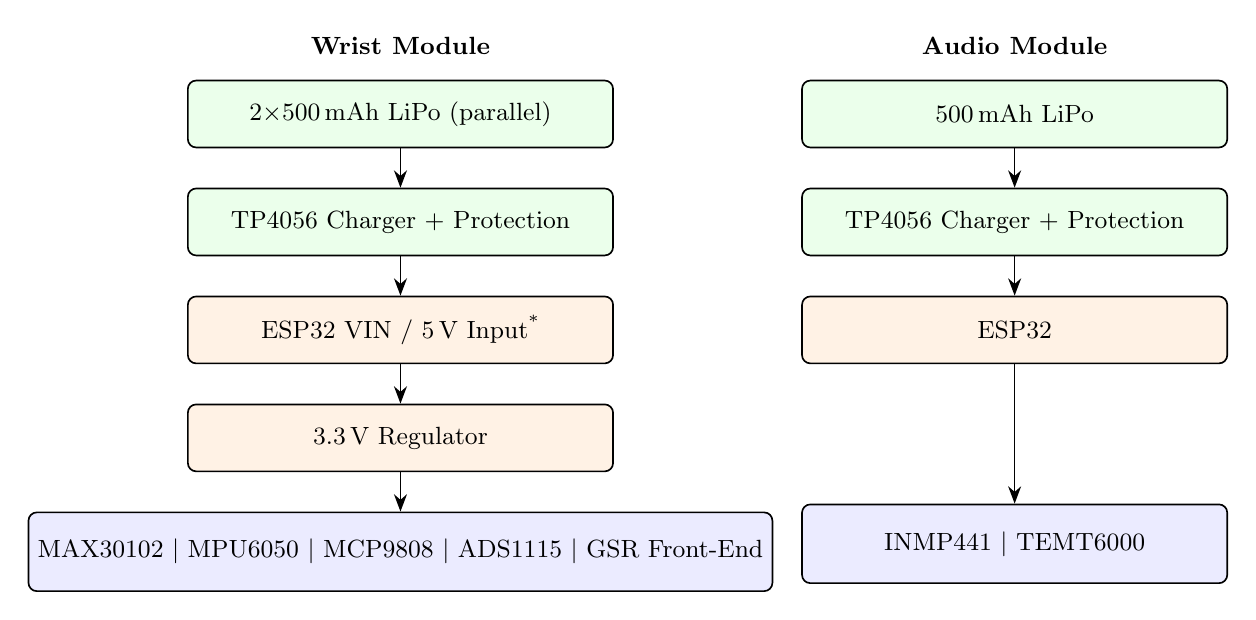
\begin{tikzpicture}[
    font=\small,
    pwrstage/.style={draw, rounded corners=3pt, minimum width=5.4cm, minimum height=0.85cm, align=center, line width=0.6pt, fill=green!8},
    ctrlstage/.style={draw, rounded corners=3pt, minimum width=5.4cm, minimum height=0.85cm, align=center, line width=0.6pt, fill=orange!10},
    loadstage/.style={draw, rounded corners=3pt, minimum width=5.4cm, minimum height=1.0cm, align=center, line width=0.6pt, fill=blue!8},
    arrow/.style={-{Stealth[length=2.2mm]}, line width=0.6pt}
]

% Wrist Module power chain
\node[pwrstage] (w1) at (0,5.2) {2$\times$500\,mAh LiPo (parallel)};
\node[pwrstage, below=5mm of w1] (w2) {TP4056 Charger + Protection};
\node[ctrlstage, below=5mm of w2] (w3) {ESP32 VIN / 5\,V Input\textsuperscript{*}};
\node[ctrlstage, below=5mm of w3] (w4) {3.3\,V Regulator};
\node[loadstage, below=5mm of w4] (w5) {MAX30102 \textbar\ MPU6050 \textbar\ MCP9808 \textbar\ ADS1115 \textbar\ GSR Front-End};

\draw[arrow] (w1.south) -- (w2.north);
\draw[arrow] (w2.south) -- (w3.north);
\draw[arrow] (w3.south) -- (w4.north);
\draw[arrow] (w4.south) -- (w5.north);

\node[above=2mm of w1, font=\bfseries\small] {Wrist Module};

% Audio Module power chain
\node[pwrstage] (a1) at (7.8,5.2) {500\,mAh LiPo};
\node[pwrstage, below=5mm of a1] (a2) {TP4056 Charger + Protection};
\node[ctrlstage, below=5mm of a2] (a3) {ESP32};
\node[loadstage, below=17.7mm of a3] (a4) {INMP441 \textbar\ TEMT6000};

\draw[arrow] (a1.south) -- (a2.north);
\draw[arrow] (a2.south) -- (a3.north);
\draw[arrow] (a3.south) -- (a4.north);

\node[above=2mm of a1, font=\bfseries\small] {Audio Module};

\end{tikzpicture}
\caption{Complete power distribution for the Wrist Module and Audio Module, from LiPo cells through the TP4056 charger/protection stage, ESP32 power input, regulation, and final sensor loads. \textsuperscript{*}Final power wiring depends on the exact ESP32 board; see the note below.}
\label{fig:power-architecture-detailed}
\end{figure*}

\begin{warningbox}
Many ESP32 DevKit boards expect a regulated 5\,V on \texttt{VIN} or USB, not a raw LiPo voltage. If powering directly from a LiPo cell, an appropriate regulator or a board designed for single-cell LiPo input is required. This must be verified on the specific board used.
\end{warningbox}

\subsection{Wrist Module GPIO Assignment}
\label{sec:wrist-gpio-assignment}

\Cref{tab:wrist-gpio} lists the GPIO assignment for the Wrist Module.

\begin{table}[H]
\centering
\caption{Wrist Module ESP32 GPIO assignment.}
\label{tab:wrist-gpio}
\small
\begin{tabularx}{\columnwidth}{@{}l Y@{}}
\toprule
\textbf{ESP32 GPIO} & \textbf{Device / Function} \\
\midrule
GPIO21 & I\textsuperscript{2}C SDA --- MAX30102, MPU6050, ADS1115, MCP9808 \\
GPIO22 & I\textsuperscript{2}C SCL --- MAX30102, MPU6050, ADS1115, MCP9808 \\
GPIO34 & ADS1115 \texttt{ALERT} (optional interrupt) \\
GPIO35 & Reserved \\
GPIO32 & Future battery monitor \\
GPIO33 & Future interrupt \\
\bottomrule
\end{tabularx}
\end{table}

\textbf{Power.} All Wrist Module sensors (MAX30102, ADS1115, MCP9808, MPU6050) are supplied from the 3.3\,V rail.

\textbf{Ground.} A common ground is shared by every module.

\subsection{Audio Module GPIO Assignment}
\label{sec:audio-gpio-assignment}

\Cref{tab:audio-gpio} lists the GPIO assignment for the Audio Module.

\begin{table}[H]
\centering
\caption{Audio Module ESP32 GPIO assignment.}
\label{tab:audio-gpio}
\small
\begin{tabularx}{\columnwidth}{@{}l Y@{}}
\toprule
\textbf{ESP32 GPIO} & \textbf{Device / Function} \\
\midrule
GPIO26 & I\textsuperscript{2}S BCLK \\
GPIO25 & I\textsuperscript{2}S LRCLK (WS) \\
GPIO33 & I\textsuperscript{2}S DATA \\
GPIO32 & TEMT6000 analog output \\
3.3\,V & Sensor VCC \\
GND & Common ground \\
\bottomrule
\end{tabularx}
\end{table}

\subsection{I\texorpdfstring{\textsuperscript{2}}{2}C Bus}
\label{sec:i2c-bus-ch5}

\Cref{fig:i2c-topology} shows the shared I\textsuperscript{2}C bus topology on the Wrist Module. \Cref{tab:i2c-addresses-ch5} lists the expected device addresses; no address conflicts are expected.

\begin{figure}[H]
\centering
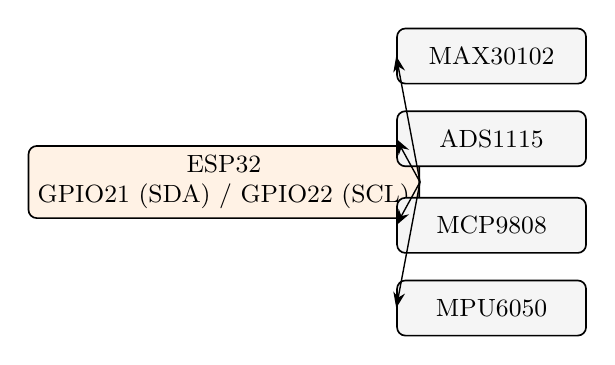
\begin{tikzpicture}[
    font=\small,
    ctrl/.style={draw, rounded corners=3pt, minimum width=2.4cm, minimum height=0.8cm, align=center, line width=0.6pt, fill=orange!10},
    dev/.style={draw, rounded corners=3pt, minimum width=2.4cm, minimum height=0.7cm, align=center, line width=0.6pt, fill=gray!8},
    arrow/.style={-{Stealth[length=2mm]}, line width=0.5pt}
]
\node[ctrl] (esp) at (0,0) {ESP32\\ GPIO21 (SDA) / GPIO22 (SCL)};

\node[dev] (max) at (3.4,1.6) {MAX30102};
\node[dev] (ads) at (3.4,0.55) {ADS1115};
\node[dev] (mcp) at (3.4,-0.55) {MCP9808};
\node[dev] (mpu) at (3.4,-1.6) {MPU6050};

\draw[arrow] (esp.east) -- (max.west);
\draw[arrow] (esp.east) -- (ads.west);
\draw[arrow] (esp.east) -- (mcp.west);
\draw[arrow] (esp.east) -- (mpu.west);
\end{tikzpicture}
\caption{Shared I\textsuperscript{2}C bus topology on the Wrist Module: the ESP32 (GPIO21/SDA, GPIO22/SCL) drives MAX30102, ADS1115, MCP9808, and MPU6050 on a single bus.}
\label{fig:i2c-topology}
\end{figure}

\begin{table}[H]
\centering
\caption{Expected I\textsuperscript{2}C device addresses on the Wrist Module bus.}
\label{tab:i2c-addresses-ch5}
\small
\begin{tabularx}{\columnwidth}{@{}Y l@{}}
\toprule
\textbf{Device} & \textbf{Address} \\
\midrule
MCP9808 & \texttt{0x18} \\
ADS1115 & \texttt{0x48} \\
MAX30102 & \texttt{0x57} \\
MPU6050 & \texttt{0x68} \\
\bottomrule
\end{tabularx}
\end{table}

\subsection{I\texorpdfstring{\textsuperscript{2}}{2}S Bus}
\label{sec:i2s-bus-ch5}

The Audio Module I\textsuperscript{2}S bus connects the ESP32 to the INMP441 digital microphone as follows: GPIO26 $\rightarrow$ BCLK, GPIO25 $\rightarrow$ WS, GPIO33 $\rightarrow$ SD, 3.3\,V $\rightarrow$ VDD, GND $\rightarrow$ GND. The INMP441 L/R select pin is connected to GND, selecting the default left channel.

\subsection{ADS1115 Connections}
\label{sec:ads1115-connections}

\Cref{tab:ads1115-wiring} lists the complete ADS1115 wiring.

\begin{table}[H]
\centering
\caption{ADS1115 pin connections.}
\label{tab:ads1115-wiring}
\small
\begin{tabularx}{\columnwidth}{@{}l Y@{}}
\toprule
\textbf{ADS1115 Pin} & \textbf{Connection} \\
\midrule
VDD & 3.3\,V \\
GND & GND \\
SDA & GPIO21 \\
SCL & GPIO22 \\
ADDR & GND (address \texttt{0x48}) \\
ALRT & Optional, GPIO34 \\
A0 & GSR front end \\
A1--A3 & Reserved \\
\bottomrule
\end{tabularx}
\end{table}

\subsection{MAX30102 Connections}
\label{sec:max30102-connections}

\Cref{tab:max30102-wiring} lists the complete MAX30102 wiring.

\begin{table}[H]
\centering
\caption{MAX30102 pin connections.}
\label{tab:max30102-wiring}
\small
\begin{tabularx}{\columnwidth}{@{}l Y@{}}
\toprule
\textbf{Sensor Pin} & \textbf{ESP32 Connection} \\
\midrule
VIN & 3.3\,V \\
GND & GND \\
SDA & GPIO21 \\
SCL & GPIO22 \\
INT & Optional, GPIO27 \\
\bottomrule
\end{tabularx}
\end{table}

\subsection{MPU6050 Connections}
\label{sec:mpu6050-connections}

\Cref{tab:mpu6050-wiring} lists the complete MPU6050 wiring. The device address is \texttt{0x68}.

\begin{table}[H]
\centering
\caption{MPU6050 pin connections.}
\label{tab:mpu6050-wiring}
\small
\begin{tabularx}{\columnwidth}{@{}l Y@{}}
\toprule
\textbf{Pin} & \textbf{ESP32 Connection} \\
\midrule
VCC & 3.3\,V \\
GND & GND \\
SDA & GPIO21 \\
SCL & GPIO22 \\
INT & Optional, GPIO14 \\
AD0 & GND \\
\bottomrule
\end{tabularx}
\end{table}

\subsection{MCP9808 Connections}
\label{sec:mcp9808-connections}

\Cref{tab:mcp9808-wiring} lists the complete MCP9808 wiring. The device address is \texttt{0x18}.

\begin{table}[H]
\centering
\caption{MCP9808 pin connections.}
\label{tab:mcp9808-wiring}
\small
\begin{tabularx}{\columnwidth}{@{}l Y@{}}
\toprule
\textbf{Pin} & \textbf{ESP32 Connection} \\
\midrule
VIN & 3.3\,V \\
GND & GND \\
SDA & GPIO21 \\
SCL & GPIO22 \\
ALERT & Optional, GPIO13 \\
A0--A2 & GND \\
\bottomrule
\end{tabularx}
\end{table}

\subsection{TEMT6000 Connections}
\label{sec:temt6000-connections}

\Cref{tab:temt6000-wiring} lists the complete TEMT6000 wiring.

\begin{table}[H]
\centering
\caption{TEMT6000 pin connections.}
\label{tab:temt6000-wiring}
\small
\begin{tabularx}{\columnwidth}{@{}l Y@{}}
\toprule
\textbf{Pin} & \textbf{ESP32 Connection} \\
\midrule
VCC & 3.3\,V \\
GND & GND \\
SIG & GPIO32 (ADC) \\
\bottomrule
\end{tabularx}
\end{table}

\subsection{GSR Front End (Current Prototype)}
\label{sec:gsr-frontend-ch5}

\Cref{fig:gsr-frontend-block} shows the current prototype signal chain for electrodermal activity acquisition.

\begin{figure}[H]
\centering
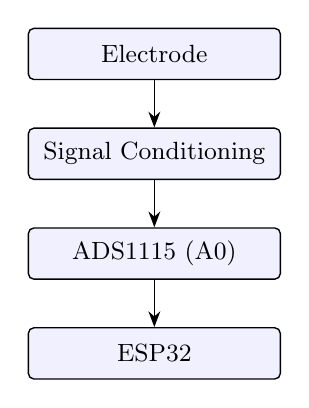
\begin{tikzpicture}[
    font=\small,
    node distance=0mm,
    field/.style={draw, rounded corners=2pt, fill=blue!6, minimum width=3.2cm, minimum height=0.65cm, align=center, line width=0.5pt}
]
\node[field] (elec) {Electrode};
\node[field, below=6mm of elec] (cond) {Signal Conditioning};
\node[field, below=6mm of cond] (ads) {ADS1115 (A0)};
\node[field, below=6mm of ads] (esp) {ESP32};

\draw[-{Stealth[length=2mm]}, line width=0.6pt] (elec.south) -- (cond.north);
\draw[-{Stealth[length=2mm]}, line width=0.6pt] (cond.south) -- (ads.north);
\draw[-{Stealth[length=2mm]}, line width=0.6pt] (ads.south) -- (esp.north);
\end{tikzpicture}
\caption{Current prototype GSR signal chain: electrode $\rightarrow$ signal conditioning $\rightarrow$ ADS1115 channel A0 $\rightarrow$ ESP32.}
\label{fig:gsr-frontend-block}
\end{figure}

\begin{requirementbox}
\textbf{Current status:} prototype implementation.
\end{requirementbox}

\begin{futureworkbox}
\textbf{Planned improvements:}
\begin{itemize}
    \item Constant-current source.
    \item RC filter.
    \item Patient protection resistor.
    \item Shielding.
    \item Calibration procedure.
\end{itemize}
\end{futureworkbox}

\subsection{Grounding Strategy}
\label{sec:grounding-strategy}

\begin{engnote}
Each module shall use a single common ground. Ground loops should be avoided, analog return paths kept short, and the microphone return path kept away from high-current power traces where possible.
\end{engnote}

\subsection{Decoupling}
\label{sec:decoupling}

\begin{designnote}
A 0.1\,\textmu F ceramic capacitor is recommended close to each sensor supply, together with a 10\,\textmu F bulk capacitor near the ESP32 power input. Additional bulk capacitance should be added if Wi-Fi brownouts are observed. Some breakout boards already include these components.
\end{designnote}

\subsection{Wiring Recommendations}
\label{sec:wiring-recommendations}

\begin{itemize}
    \item Use 26--28\,AWG stranded wire for power.
    \item Use 28--30\,AWG stranded wire for signal wiring.
    \item Keep I\textsuperscript{2}C runs short.
    \item Use twisted-pair or closely routed GSR leads if cable length increases.
    \item Provide secure strain relief for battery and sensor connections.
\end{itemize}

\subsection{Electrical Safety}
\label{sec:electrical-safety}

\begin{warningbox}
\begin{itemize}
    \item Never apply 5\,V directly to ESP32 GPIO pins.
    \item Verify battery polarity before connecting.
    \item Do not charge the module while connected to GSR electrodes.
    \item Insulate all exposed battery terminals.
    \item Disconnect power before rewiring.
    \item Inspect LiPo cells before every test.
\end{itemize}
\end{warningbox}

\subsection{Estimated Current Budget}
\label{sec:current-budget}

\Cref{tab:current-budget} lists the estimated per-device current draw for both modules. The Wrist Module total is estimated at $\approx$90--210+\,mA, and the Audio Module total at $\approx$85--205+\,mA.

\begin{table}[H]
\centering
\caption{Estimated current budget by module and device.}
\label{tab:current-budget}
\small
\begin{tabularx}{\columnwidth}{@{}l l Y@{}}
\toprule
\textbf{Module} & \textbf{Device} & \textbf{Approx. Current} \\
\midrule
Wrist & ESP32 & 80--200\,mA (Wi-Fi/CPU dependent) \\
Wrist & MAX30102 & 1--5\,mA \\
Wrist & MPU6050 & 3--5\,mA \\
Wrist & ADS1115 & \textless 1\,mA \\
Wrist & MCP9808 & \textless 1\,mA \\
Wrist & GSR front end & Depends on final circuit \\
\midrule
Audio & ESP32 & 80--200\,mA \\
Audio & INMP441 & 1--2\,mA \\
Audio & TEMT6000 & \textless 1\,mA \\
\bottomrule
\end{tabularx}
\end{table}

\subsection{Remaining Electrical Validation}
\label{sec:remaining-electrical-validation}

\begin{requirementbox}
\textbf{The following must still be verified on the assembled hardware:}
\begin{itemize}
    \item Exact ESP32 power input path and acceptable VIN range.
    \item 3.3\,V rail stability under Wi-Fi load.
    \item Battery runtime under continuous operation.
    \item Charge current of the TP4056 (PROG resistor).
    \item Brownout threshold.
    \item Peak current during wireless transmission.
    \item Thermal performance during charging.
    \item Final GPIO validation with firmware.
\end{itemize}
\end{requirementbox}

\subsection{Chapter Status}
\label{sec:ch5-status}

\begin{validationbox}
\textbf{Completed for this chapter:}
\begin{itemize}
    \item Complete wiring architecture
    \item GPIO assignments
    \item I\textsuperscript{2}C wiring
    \item I\textsuperscript{2}S wiring
    \item Power distribution
    \item Grounding strategy
    \item Current budget
    \item Electrical safety
    \item Integration notes
\end{itemize}
\end{validationbox}


% ============================================================
% CHAPTER 6
% ============================================================
% ============================================================
% Chapter 6 — Firmware Architecture & Software Design
% Source: PSYCON Engineering Design Document, Vol. 1, Ch. 6
% ============================================================
\section{Firmware Architecture \& Software Design}
\label{sec:firmware-architecture}

\subsection{Firmware Overview}
\label{sec:firmware-overview}

PSYCON uses two independent ESP32 firmware projects, one per module.

\textbf{Wrist Module firmware} is responsible for: MAX30102 acquisition; MPU6050 acquisition; MCP9808 acquisition; GSR acquisition (via the ADS1115); timestamping; local preprocessing; BLE/Wi-Fi transmission; battery monitoring; and error logging.

\textbf{Audio Module firmware} is responsible for: INMP441 audio capture; TEMT6000 acquisition; audio buffering; voice preprocessing; BLE/Wi-Fi transmission; battery monitoring; and error logging.

\subsection{Software Layers}
\label{sec:software-layers}

\Cref{fig:software-layers} shows the layered firmware architecture shared by both modules, from the application layer down to the physical ESP32 hardware.

\begin{figure}[H]
\centering
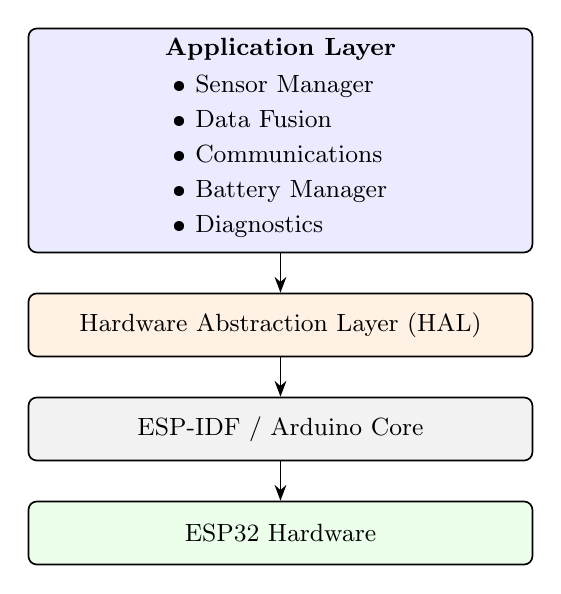
\begin{tikzpicture}[
    font=\small,
    node distance=0mm,
    layer/.style={draw, rounded corners=3pt, minimum width=6.4cm, align=center, line width=0.6pt},
    apps/.style={layer, fill=blue!8, minimum height=1.9cm},
    hal/.style={layer, fill=orange!10, minimum height=0.8cm},
    core/.style={layer, fill=gray!10, minimum height=0.8cm},
    hw/.style={layer, fill=green!8, minimum height=0.8cm}
]
\node[apps] (app) {
  \textbf{Application Layer}\\[2pt]
  \begin{tabular}{@{}l@{}}
  \textbullet\ Sensor Manager \\
  \textbullet\ Data Fusion \\
  \textbullet\ Communications \\
  \textbullet\ Battery Manager \\
  \textbullet\ Diagnostics
  \end{tabular}
};
\node[hal, below=5mm of app] (hal) {Hardware Abstraction Layer (HAL)};
\node[core, below=5mm of hal] (core) {ESP-IDF / Arduino Core};
\node[hw, below=5mm of core] (hw) {ESP32 Hardware};

\draw[-{Stealth[length=2mm]}, line width=0.6pt] (app.south) -- (hal.north);
\draw[-{Stealth[length=2mm]}, line width=0.6pt] (hal.south) -- (core.north);
\draw[-{Stealth[length=2mm]}, line width=0.6pt] (core.south) -- (hw.north);
\end{tikzpicture}
\caption{Layered firmware architecture: an application layer (sensor management, data fusion, communications, battery management, diagnostics) sits above a hardware abstraction layer, the ESP-IDF/Arduino core, and the ESP32 hardware itself.}
\label{fig:software-layers}
\end{figure}

\subsection{Wrist Module Tasks}
\label{sec:wrist-module-tasks}

The Wrist Module firmware is organized into eight cooperating tasks, summarized in \Cref{tab:wrist-tasks-summary} and illustrated in \Cref{fig:wrist-task-pipeline}.

\begin{table*}[t]
\centering
\caption{Wrist Module firmware task summary.}
\label{tab:wrist-tasks-summary}
\small
\begin{tabularx}{\textwidth}{@{}l l Y@{}}
\toprule
\textbf{Task} & \textbf{Trigger} & \textbf{Responsibilities} \\
\midrule
1. Sensor Initialization & Runs once & Initializes MAX30102, ADS1115, MPU6050, MCP9808 \\
2. Heart Rate Task & Periodic & Reads RED LED; reads IR LED; filters signal; stores buffer \\
3. Motion Task & Periodic & Reads accelerometer and gyroscope; computes movement and orientation \\
4. Temperature Task & Periodic & Reads MCP9808; stores temperature \\
5. GSR Task & Periodic & Reads ADS1115; converts ADC value to conductance; stores value \\
6. Packet Builder & Periodic & Assembles one packet from timestamp, heart, motion, temperature, GSR, and checksum \\
7. BLE/Wi-Fi Task & Periodic & Uploads packets; retries on failure \\
8. Battery Monitor & Periodic & Checks battery voltage; issues low-battery / shutdown warnings \\
\bottomrule
\end{tabularx}
\end{table*}

\begin{figure*}[t]
\centering
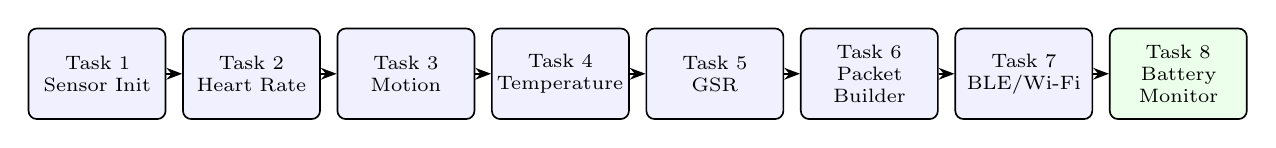
\begin{tikzpicture}[
    font=\scriptsize,
    stage/.style={draw, rounded corners=3pt, text width=1.6cm, minimum height=1.15cm, align=center, line width=0.6pt, fill=blue!6, inner sep=2pt},
    final/.style={stage, fill=green!8},
    arrow/.style={-{Stealth[length=2mm]}, line width=0.6pt},
    node distance=2mm
]
\node[stage] (t1) {Task 1\\Sensor Init};
\node[stage, right=of t1] (t2) {Task 2\\Heart Rate};
\node[stage, right=of t2] (t3) {Task 3\\Motion};
\node[stage, right=of t3] (t4) {Task 4\\Temperature};
\node[stage, right=of t4] (t5) {Task 5\\GSR};
\node[stage, right=of t5] (t6) {Task 6\\Packet Builder};
\node[stage, right=of t6] (t7) {Task 7\\BLE/Wi-Fi};
\node[final, right=of t7] (t8) {Task 8\\Battery Monitor};

\draw[arrow] (t1.east) -- (t2.west);
\draw[arrow] (t2.east) -- (t3.west);
\draw[arrow] (t3.east) -- (t4.west);
\draw[arrow] (t4.east) -- (t5.west);
\draw[arrow] (t5.east) -- (t6.west);
\draw[arrow] (t6.east) -- (t7.west);
\draw[arrow] (t7.east) -- (t8.west);
\end{tikzpicture}
\caption{Wrist Module task pipeline: one-time sensor initialization followed by periodic acquisition tasks (heart rate, motion, temperature, GSR), packet assembly, wireless upload, and battery monitoring.}
\label{fig:wrist-task-pipeline}
\end{figure*}

\subsection{Audio Tasks}
\label{sec:audio-tasks-ch6}

The Audio Module firmware runs four cooperating tasks: the Microphone Task, the Light Sensor Task, the Packet Builder, and the Battery Monitor / Communication task. \Cref{fig:audio-task-pipeline} shows the audio acquisition pipeline from initialization through transmission.

\begin{figure}[H]
\centering
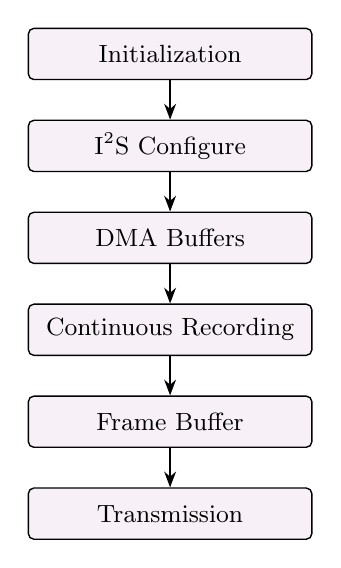
\begin{tikzpicture}[
    font=\small,
    node distance=0mm,
    field/.style={draw, rounded corners=2pt, fill=violet!6, minimum width=3.6cm, minimum height=0.65cm, align=center, line width=0.5pt}
]
\node[field] (init) {Initialization};
\node[field, below=5mm of init] (i2s) {I\textsuperscript{2}S Configure};
\node[field, below=5mm of i2s] (dma) {DMA Buffers};
\node[field, below=5mm of dma] (rec) {Continuous Recording};
\node[field, below=5mm of rec] (frame) {Frame Buffer};
\node[field, below=5mm of frame] (tx) {Transmission};

\foreach \a/\b in {init/i2s, i2s/dma, dma/rec, rec/frame, frame/tx}
  \draw[-{Stealth[length=2mm]}, line width=0.6pt] (\a.south) -- (\b.north);
\end{tikzpicture}
\caption{Audio Module acquisition pipeline: initialization, I\textsuperscript{2}S configuration, DMA buffer setup, continuous recording, frame buffering, and transmission.}
\label{fig:audio-task-pipeline}
\end{figure}

\subsection{Data Flow}
\label{sec:firmware-data-flow}

\Cref{fig:firmware-data-flow} shows the end-to-end firmware data flow, from raw sensor reads through to server-side AI processing.

\begin{figure*}[t]
\centering
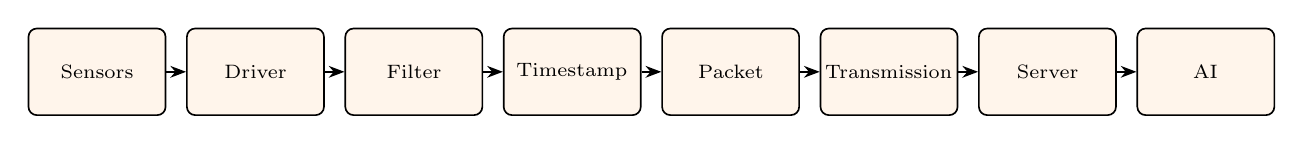
\begin{tikzpicture}[
    font=\scriptsize,
    stage/.style={draw, rounded corners=3pt, text width=1.6cm, minimum height=1.1cm, align=center, line width=0.6pt, fill=orange!8, inner sep=2pt},
    arrow/.style={-{Stealth[length=2mm]}, line width=0.6pt},
    node distance=2.5mm
]
\node[stage] (s1) {Sensors};
\node[stage, right=of s1] (s2) {Driver};
\node[stage, right=of s2] (s3) {Filter};
\node[stage, right=of s3] (s4) {Timestamp};
\node[stage, right=of s4] (s5) {Packet};
\node[stage, right=of s5] (s6) {Transmission};
\node[stage, right=of s6] (s7) {Server};
\node[stage, right=of s7] (s8) {AI};

\foreach \i/\j in {s1/s2, s2/s3, s3/s4, s4/s5, s5/s6, s6/s7, s7/s8}
  \draw[arrow] (\i.east) -- (\j.west);
\end{tikzpicture}
\caption{End-to-end firmware data flow, from sensor acquisition through driver-level reads, filtering, timestamping, packet assembly, wireless transmission, server ingestion, and AI processing.}
\label{fig:firmware-data-flow}
\end{figure*}

\subsection{Packet Structure}
\label{sec:packet-structure}

\Cref{tab:packet-physio} lists an example physiological packet structure (Wrist Module), and \Cref{tab:packet-audio} lists the audio packet structure (Audio Module).

\begin{table}[H]
\centering
\caption{Example physiological (Wrist Module) packet fields.}
\label{tab:packet-physio}
\small
\begin{tabularx}{\columnwidth}{@{}l Y@{}}
\toprule
\textbf{\#} & \textbf{Field} \\
\midrule
1 & Timestamp \\
2 & Heart rate \\
3 & SpO\textsubscript{2} \\
4 & Accelerometer X \\
5 & Accelerometer Y \\
6 & Accelerometer Z \\
7 & Gyroscope X \\
8 & Gyroscope Y \\
9 & Gyroscope Z \\
10 & Temperature \\
11 & GSR \\
12 & Battery \\
13 & Checksum \\
\bottomrule
\end{tabularx}
\end{table}

\begin{table}[H]
\centering
\caption{Audio packet fields.}
\label{tab:packet-audio}
\small
\begin{tabularx}{\columnwidth}{@{}l Y@{}}
\toprule
\textbf{\#} & \textbf{Field} \\
\midrule
1 & Timestamp \\
2 & PCM samples \\
3 & Battery \\
4 & Checksum \\
\bottomrule
\end{tabularx}
\end{table}

\subsection{Sampling Strategy}
\label{sec:sampling-strategy}

\Cref{tab:sampling-strategy} summarizes the acquisition regime for each signal. Actual sampling frequencies are to be finalized based on testing and downstream processing requirements.

\begin{table}[H]
\centering
\caption{Sampling strategy by signal.}
\label{tab:sampling-strategy}
\small
\begin{tabularx}{\columnwidth}{@{}Y l@{}}
\toprule
\textbf{Signal} & \textbf{Regime} \\
\midrule
Heart & Continuous \\
Motion & Continuous \\
Temperature & Periodic \\
Light & Periodic \\
Audio & Continuous \\
GSR & Continuous \\
\bottomrule
\end{tabularx}
\end{table}

\begin{requirementbox}
Actual sampling frequencies for each signal remain to be finalized based on empirical testing and the requirements of downstream processing.
\end{requirementbox}

\subsection{Error Handling}
\label{sec:error-handling-ch6}

\Cref{alg:error-handling} describes the generic sensor error-handling procedure used across both firmware projects. The system is designed so that a single failed sensor never causes a complete crash.

\begin{algorithm}[t]
\small
\caption{Generic Sensor Error Handling}
\label{alg:error-handling}
\KwData{Sensor read request}
\KwResult{Sensor value or logged failure, without halting the system}
Attempt sensor read\;
\If{timeout or communication error detected}{
  Retry read\;
  \If{retry fails}{
    Log error (sensor ID, error type, timestamp)\;
  }
}
Continue acquisition for all remaining sensors\;
\end{algorithm}

\subsection{Communication}
\label{sec:communication-ch6}

Every transmitted packet contains: a timestamp; a sensor ID; the payload; a CRC/checksum; and a sequence number. Because each packet carries a sequence number, missing packets can be detected at the receiving end.

\subsection{Logging}
\label{sec:logging-ch6}

The firmware maintains logs for: sensor initialization failures; I\textsuperscript{2}C communication errors; buffer overruns; Wi-Fi/BLE reconnects; battery warnings; brownout events; and memory allocation failures.

\subsection{Battery Management}
\label{sec:battery-management-ch6}

\Cref{fig:battery-state} shows the firmware battery-management state progression. Sudden power loss is avoided where possible by saving pending data before shutdown.

\begin{figure}[H]
\centering
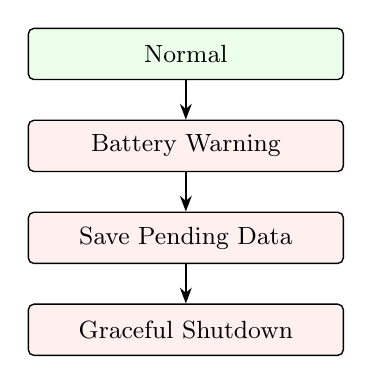
\begin{tikzpicture}[
    font=\small,
    node distance=0mm,
    field/.style={draw, rounded corners=2pt, fill=red!6, minimum width=4.0cm, minimum height=0.65cm, align=center, line width=0.5pt}
]
\node[field, fill=green!8] (normal) {Normal};
\node[field, below=5mm of normal] (warn) {Battery Warning};
\node[field, below=5mm of warn] (save) {Save Pending Data};
\node[field, below=5mm of save] (shut) {Graceful Shutdown};

\foreach \a/\b in {normal/warn, warn/save, save/shut}
  \draw[-{Stealth[length=2mm]}, line width=0.6pt] (\a.south) -- (\b.north);
\end{tikzpicture}
\caption{Firmware battery-management state progression, from normal operation through a battery-warning state, saving of pending data, and graceful shutdown.}
\label{fig:battery-state}
\end{figure}

\subsection{Boot Sequence}
\label{sec:boot-sequence}

\Cref{fig:boot-sequence} shows the firmware boot sequence, from power-on to continuous acquisition.

\begin{figure}[H]
\centering
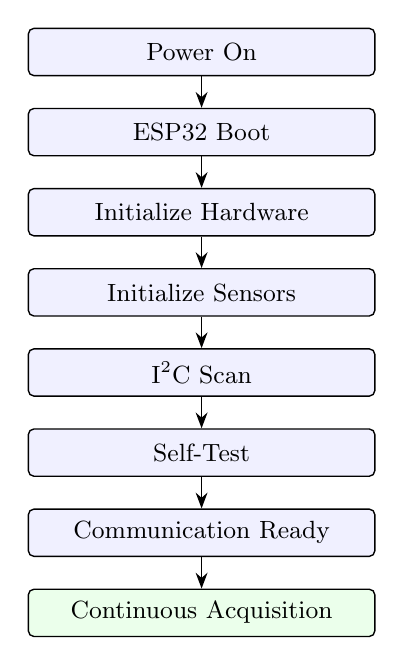
\begin{tikzpicture}[
    font=\small,
    node distance=0mm,
    field/.style={draw, rounded corners=2pt, fill=blue!6, minimum width=4.4cm, minimum height=0.6cm, align=center, line width=0.5pt}
]
\node[field] (pwr) {Power On};
\node[field, below=4mm of pwr] (boot) {ESP32 Boot};
\node[field, below=4mm of boot] (hwinit) {Initialize Hardware};
\node[field, below=4mm of hwinit] (sensinit) {Initialize Sensors};
\node[field, below=4mm of sensinit] (scan) {I\textsuperscript{2}C Scan};
\node[field, below=4mm of scan] (self) {Self-Test};
\node[field, below=4mm of self] (comm) {Communication Ready};
\node[field, below=4mm of comm, fill=green!8] (acq) {Continuous Acquisition};

\foreach \a/\b in {pwr/boot, boot/hwinit, hwinit/sensinit, sensinit/scan, scan/self, self/comm, comm/acq}
  \draw[-{Stealth[length=2mm]}, line width=0.6pt] (\a.south) -- (\b.north);
\end{tikzpicture}
\caption{Firmware boot sequence, from power-on through hardware and sensor initialization, an I\textsuperscript{2}C bus scan, self-test, and communication readiness, to continuous acquisition.}
\label{fig:boot-sequence}
\end{figure}

\subsection{Watchdog Recovery}
\label{sec:watchdog-recovery}

\begin{engnote}
If the firmware hangs, the watchdog resets the ESP32. The boot reason is logged, and data acquisition resumes automatically after restart.
\end{engnote}

\subsection{Memory Management}
\label{sec:memory-management-ch6}

\begin{designnote}
Firmware uses fixed-size buffers and circular/ring buffers for continuous streams. Dynamic memory allocation (\texttt{malloc}/\texttt{new}) is avoided within continuous acquisition loops to reduce heap fragmentation.
\end{designnote}

\subsection{Audio Buffering}
\label{sec:audio-buffering}

\Cref{fig:audio-buffering} shows the audio buffering chain, which helps prevent sample loss during temporary communication delays.

\begin{figure}[H]
\centering
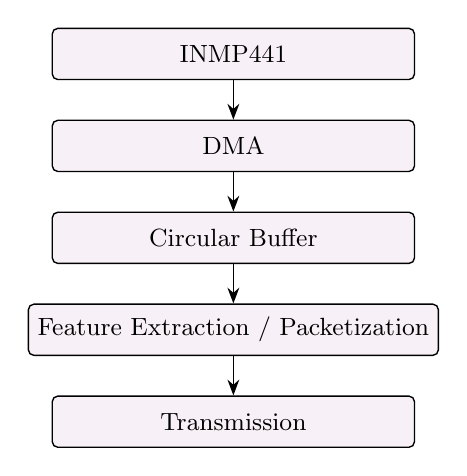
\begin{tikzpicture}[
    font=\small,
    node distance=0mm,
    field/.style={draw, rounded corners=2pt, fill=violet!6, minimum width=4.6cm, minimum height=0.65cm, align=center, line width=0.5pt}
]
\node[field] (mic) {INMP441};
\node[field, below=5mm of mic] (dma) {DMA};
\node[field, below=5mm of dma] (circ) {Circular Buffer};
\node[field, below=5mm of circ] (feat) {Feature Extraction / Packetization};
\node[field, below=5mm of feat] (tx) {Transmission};

\foreach \a/\b in {mic/dma, dma/circ, circ/feat, feat/tx}
  \draw[-{Stealth[length=2mm]}, line width=0.6pt] (\a.south) -- (\b.north);
\end{tikzpicture}
\caption{Audio buffering chain from the INMP441 microphone through DMA and a circular buffer to feature extraction/packetization and transmission, reducing sample loss during transient communication delays.}
\label{fig:audio-buffering}
\end{figure}

\subsection{Firmware Folder Structure}
\label{sec:firmware-folder-structure}

\Cref{lst:firmware-structure} shows the planned firmware repository layout, shared between the Wrist and Audio Module projects.

\begin{figure}[H]
\centering
\begin{lstlisting}[
  basicstyle=\ttfamily\scriptsize,
  frame=single,
  caption={PSYCON firmware repository structure.},
  label={lst:firmware-structure},
  numbers=none
]
firmware/
|-- wrist/
|   |-- sensors/
|   |-- communication/
|   |-- battery/
|   |-- logging/
|   |-- utilities/
|   `-- main.cpp
|-- audio/
|   |-- microphone/
|   |-- communication/
|   |-- battery/
|   |-- logging/
|   `-- main.cpp
`-- shared/
    |-- config.h
    |-- packet.h
    |-- crc.cpp
    `-- timestamp.cpp
\end{lstlisting}
\end{figure}

\subsection{Firmware Validation Checklist}
\label{sec:firmware-validation-checklist}

\begin{requirementbox}
\textbf{Before full integration, the following must be verified:}
\begin{itemize}
    \item Sensor initialization succeeds.
    \item All I\textsuperscript{2}C devices are detected.
    \item No address conflicts.
    \item Stable sampling over extended periods.
    \item No packet corruption.
    \item No memory leaks.
    \item No watchdog resets during normal operation.
    \item Battery warnings trigger correctly.
    \item Graceful shutdown works.
    \item Audio stream remains continuous without excessive buffer overruns.
\end{itemize}
\end{requirementbox}

\subsection{Version Control}
\label{sec:version-control-ch6}

The following are tracked under version control: firmware version; hardware revision; configuration changes; sensor calibration updates; release notes; and test results for each firmware version.

\subsection{Chapter Status}
\label{sec:ch6-status}

\begin{validationbox}
\textbf{Completed for this chapter:}
\begin{itemize}
    \item Firmware architecture
    \item Task scheduling
    \item Sensor acquisition flow
    \item Packet structure
    \item Communication design
    \item Logging strategy
    \item Battery management
    \item Error handling
    \item Memory management
    \item Boot process
    \item Validation checklist
\end{itemize}
\end{validationbox}


% ============================================================
% CHAPTER 7
% ============================================================
% ============================================================
% Chapter 7 — AI Pipeline, Backend Architecture & Machine Learning Design
% Source: PSYCON Engineering Design Document, Vol. 1, Ch. 7
% ============================================================
\section{AI Pipeline, Backend Architecture \& Machine Learning Design}
\label{sec:ai-pipeline-design}

\subsection{AI System Overview}
\label{sec:ai-system-overview}

PSYCON consists of two synchronized AI pipelines whose feature sets are fused into a final inference engine.

\textbf{Physiological AI Pipeline.} Heart rate; heart rate variability (HRV); blood-oxygen trends (SpO\textsubscript{2}, if used); galvanic skin response (GSR/EDA); body temperature; motion/activity.

\textbf{Speech AI Pipeline.} Voice recording; speech characteristics; language features; conversation analysis; acoustic features.

\subsection{Overall Architecture}
\label{sec:ai-overall-architecture}

\Cref{fig:ai-overall-architecture} shows how physiological features from the Wrist Module and speech features from the Audio Module converge in the AI fusion engine.

\begin{figure}[H]
\centering
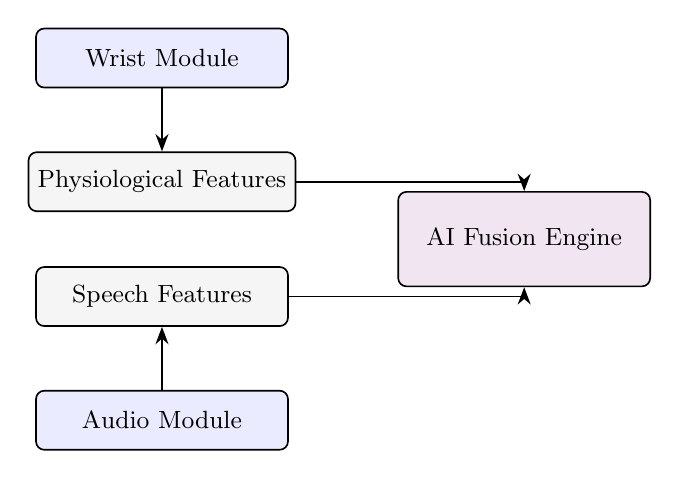
\begin{tikzpicture}[
    font=\small,
    stage/.style={draw, rounded corners=3pt, minimum width=3.2cm, minimum height=0.75cm, align=center, line width=0.6pt},
    mod/.style={stage, fill=blue!8},
    feat/.style={stage, fill=gray!8},
    fuse/.style={stage, fill=violet!10, minimum width=3.2cm, minimum height=1.2cm},
    arrow/.style={-{Stealth[length=2.2mm]}, line width=0.6pt}
]
\node[mod] (wrist) at (0,4.6) {Wrist Module};
\node[feat, below=8mm of wrist] (physfeat) {Physiological Features};

\node[mod] (audio) at (0,0) {Audio Module};
\node[feat, above=8mm of audio] (speechfeat) {Speech Features};

\node[fuse] (fusion) at (4.6,2.3) {AI Fusion Engine};

\draw[arrow] (wrist.south) -- (physfeat.north);
\draw[arrow] (audio.north) -- (speechfeat.south);
\draw[arrow] (physfeat.east) -| (fusion.north);
\draw[arrow] (speechfeat.east) -| (fusion.south);
\end{tikzpicture}
\caption{Overall AI architecture: physiological features from the Wrist Module and speech features from the Audio Module converge in the AI fusion engine.}
\label{fig:ai-overall-architecture}
\end{figure}

\subsection{Data Acquisition}
\label{sec:data-acquisition-ai}

\textbf{Physiological.} Heart rate, HRV, GSR, temperature, and motion are collected continuously. Every sample receives a timestamp, sensor ID, quality flag, and battery status.

\textbf{Speech.} The target system collects consented speech continuously in an approved study. The current firmware has not yet demonstrated continuous capture; \Cref{fig:speech-pipeline} shows the intended acquisition pipeline.

\begin{figure}[H]
\centering
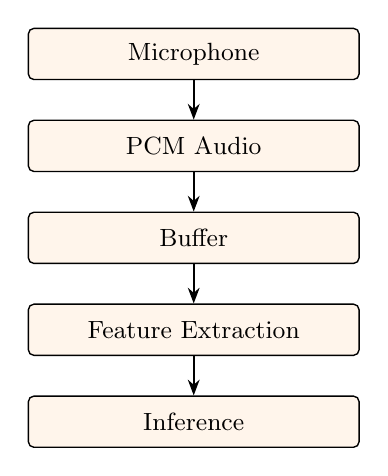
\begin{tikzpicture}[
    font=\small,
    node distance=0mm,
    field/.style={draw, rounded corners=2pt, fill=orange!8, minimum width=4.2cm, minimum height=0.65cm, align=center, line width=0.5pt}
]
\node[field] (mic) {Microphone};
\node[field, below=5mm of mic] (pcm) {PCM Audio};
\node[field, below=5mm of pcm] (buf) {Buffer};
\node[field, below=5mm of buf] (feat) {Feature Extraction};
\node[field, below=5mm of feat] (inf) {Inference};

\foreach \a/\b in {mic/pcm, pcm/buf, buf/feat, feat/inf}
  \draw[-{Stealth[length=2mm]}, line width=0.6pt] (\a.south) -- (\b.north);
\end{tikzpicture}
\caption{Speech acquisition pipeline: microphone $\rightarrow$ PCM audio $\rightarrow$ buffer $\rightarrow$ feature extraction $\rightarrow$ inference.}
\label{fig:speech-pipeline}
\end{figure}

\subsection{Feature Engineering}
\label{sec:feature-engineering}

\Cref{tab:feature-engineering} summarizes candidate features under consideration for each signal modality.

\begin{table*}[t]
\centering
\caption{Candidate features by signal modality.}
\label{tab:feature-engineering}
\small
\begin{tabularx}{\textwidth}{@{}l Y@{}}
\toprule
\textbf{Modality} & \textbf{Candidate Features} \\
\midrule
Heart & Mean HR; HR variability; resting trend; peak frequency; recovery trend \\
Motion & Activity level; tremor; stability; walking; rest periods \\
Temperature & Mean; drift; sudden changes; long-term baseline \\
GSR & Baseline conductance; slow tonic changes; rapid phasic responses; peak count; recovery slope \\
Speech (acoustic) & Speaking rate; pause duration; pitch statistics; energy/loudness; voice stability; spectral features (e.g., MFCCs) \\
Speech (language) & Vocabulary diversity; sentence length; sentiment; emotion-related language; topic transitions \\
\bottomrule
\end{tabularx}
\end{table*}

\begin{researchnote}
The feature lists above represent candidate features under consideration. Final feature selection should be informed by empirical validation on collected data.
\end{researchnote}

\subsection{Implemented Audio Engineering Baseline}
\label{sec:implemented-audio-baseline}

The software implements one deterministic mono PCM16 extractor named \texttt{psycon\_audio}. Its ordered feature vector contains duration, RMS and peak dBFS, clipping fraction, DC offset, zero-crossing rate, spectral centroid, 85\% spectral rolloff, spectral flatness, mean/standard-deviation/minimum/maximum autocorrelation pitch from 70--400~Hz, relative pitch jitter, bounded voice stability, energy-active frame fraction, pause count, and pause duration. It has no downloaded-model or third-party feature-extractor dependency. Feature changes must update the contract and equivalence tests together.

Every extracted window retains the session and device identifiers, packet sequence, device timestamp, first sample index, sample count, nominal sample rate, SHA-256 source-packet digest, and extractor identity. Before inference, the pipeline returns one explicit state: usable, insufficient audio, clipped, too noisy, corrupt, or missing audio. Missing input is never replaced with zero-valued audio.

Deterministic fixtures cover silence, impulse, a 220~Hz tone, clipped tone, amplitude-modulated speech-like input, and seeded white noise. The local demo passes each fixture through the Protocol v2 decoder and writes a JSON decision report. These tests verify the software contract and abstention behavior only; final thresholds require evidence from the installed INMP441, and continuous capture, light alignment, clock behavior, and transport-loss recovery remain physical integration gates.

The consent-gated \texttt{psycon\_transcription} stage transcribes contiguous acoustic windows marked usable with a locally cached faster-whisper model; rejected windows never silently enter speech-to-text processing. Results preserve timestamped transcript segments, source-sample boundaries, detected language, approximate confidence, engine/model identity, and explicit complete, no-speech, skipped-quality, unavailable, not-requested, or failed states. Recordings are not sent to a third-party transcription API.

The development profile uses the multilingual \texttt{small} model on CPU with int8 computation, replacing \texttt{tiny} because transcript errors directly contaminate downstream language features. The approved production profile runs multilingual \texttt{turbo} with float16 computation on a CUDA GPU inside the PSYCON backend. The model, device, and compute type are deployment configuration and must be recorded with every result.

Before release, compare \texttt{small}, \texttt{medium}, and \texttt{turbo} on representative consented multilingual recordings. Report per-language word or character error rate, language-detection accuracy, end-to-end latency, peak memory, failure rate, and stability of downstream language features. Freeze the selected model only after this evidence is recorded; a server deployment does not waive latency, concurrency, cost, or privacy constraints.

The \texttt{psycon\_language} baseline implements the English features specified in this chapter: vocabulary diversity, sentence count and length, transparent lexicon-based sentiment, emotion-related word counts, topic-transition distance, speech duration, pause duration, and speaking rate. The transcription layer accepts multilingual speech, but the language-feature extractor explicitly abstains for non-English transcripts until validated language-specific tokenization and lexicons exist. Insufficient text and unavailable transcription also abstain explicitly. These features are intended for controlled research comparison; they are not validated emotion recognition, speaker diarization, or clinical interpretation.

The local webpage accepts permission-confirmed WAV recordings, performs decoding and balanced Protocol v2 quality windows of at most two seconds, optionally runs local transcription, and displays acoustic decisions, transcript segments, language features, and provenance. Its permission checkbox is an engineering safeguard rather than a complete participant-consent system, and the localhost development server is not a production data-collection service.

\subsection{Data Fusion}
\label{sec:data-fusion-ai}

The backend aligns sensor and speech data using timestamps. \Cref{fig:data-fusion} shows the fusion process from sensor and speech features to a combined feature vector and the inference engine.

\begin{figure}[H]
\centering
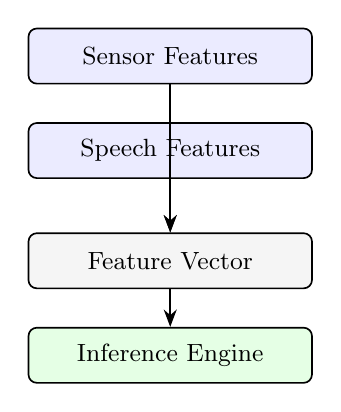
\begin{tikzpicture}[
    font=\small,
    stage/.style={draw, rounded corners=3pt, minimum width=3.6cm, minimum height=0.7cm, align=center, line width=0.6pt},
    src/.style={stage, fill=blue!8},
    vec/.style={stage, fill=gray!8},
    inf/.style={stage, fill=green!10},
    arrow/.style={-{Stealth[length=2.2mm]}, line width=0.6pt}
]
\node[src] (sf) at (0,2.4) {Sensor Features};
\node[src] (spf) at (0,1.2) {Speech Features};
\node[vec] (fv) at (0,-0.2) {Feature Vector};
\node[inf] (ie) at (0,-1.4) {Inference Engine};

\draw[arrow] (sf.south) -- ++(0,-4mm) -| (fv.north);
\draw[arrow] (spf.south) -- (fv.north);
\draw[arrow] (fv.south) -- (ie.north);
\end{tikzpicture}
\caption{Data fusion: timestamp-aligned sensor and speech features are combined into a single feature vector for the inference engine.}
\label{fig:data-fusion}
\end{figure}

\subsection{Backend Components}
\label{sec:backend-components}

\Cref{fig:backend-pipeline} shows the end-to-end backend pipeline, from device data ingestion to the user-facing dashboard.

\begin{figure*}[t]
\centering
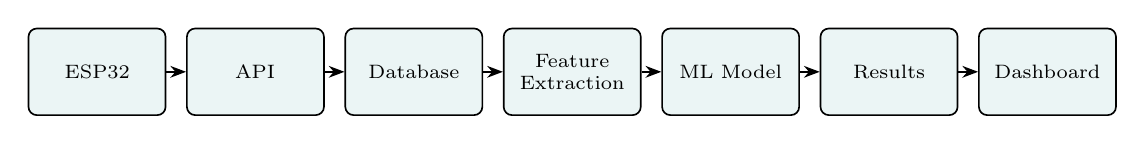
\begin{tikzpicture}[
    font=\scriptsize,
    stage/.style={draw, rounded corners=3pt, text width=1.6cm, minimum height=1.1cm, align=center, line width=0.6pt, fill=teal!8, inner sep=2pt},
    arrow/.style={-{Stealth[length=2mm]}, line width=0.6pt},
    node distance=2.5mm
]
\node[stage] (s1) {ESP32};
\node[stage, right=of s1] (s2) {API};
\node[stage, right=of s2] (s3) {Database};
\node[stage, right=of s3] (s4) {Feature Extraction};
\node[stage, right=of s4] (s5) {ML Model};
\node[stage, right=of s5] (s6) {Results};
\node[stage, right=of s6] (s7) {Dashboard};

\foreach \i/\j in {s1/s2, s2/s3, s3/s4, s4/s5, s5/s6, s6/s7}
  \draw[arrow] (\i.east) -- (\j.west);
\end{tikzpicture}
\caption{End-to-end backend pipeline, from ESP32 device data through the API and database, feature extraction, ML model inference, and results, to the user-facing dashboard.}
\label{fig:backend-pipeline}
\end{figure*}

\subsection{Database Structure}
\label{sec:database-structure}

\Cref{tab:database-structure} lists the fields stored for each session.

\begin{table}[H]
\centering
\caption{Fields stored per session.}
\label{tab:database-structure}
\small
\begin{tabularx}{\columnwidth}{@{}Y@{}}
\toprule
\textbf{Field} \\
\midrule
User ID \\
Session ID \\
Timestamp \\
Sensor data \\
Audio metadata \\
Extracted features \\
Model output \\
Confidence score \\
Logs \\
\bottomrule
\end{tabularx}
\end{table}

\begin{warningbox}
For privacy, avoid storing raw audio longer than necessary unless explicit user consent and a clear research need are established. Server-side transcription requires encrypted transport and storage, authenticated access, audit logging, a documented retention and deletion schedule, and separation of participant identity from recordings and transcripts.
\end{warningbox}

\subsection{Machine Learning Workflow}
\label{sec:ml-workflow}

\Cref{fig:ml-workflow} shows the end-to-end machine learning workflow, from raw data collection through to inference.

\begin{figure}[H]
\centering
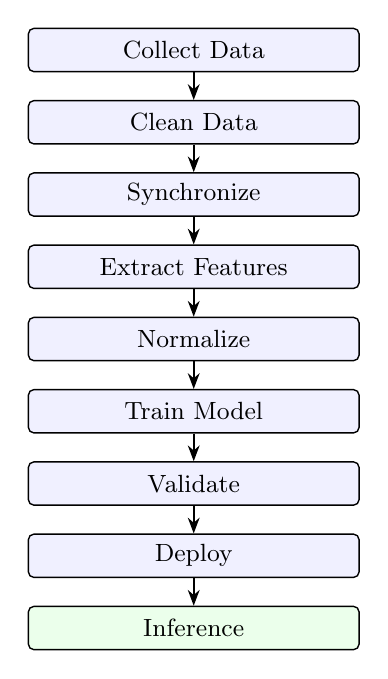
\begin{tikzpicture}[
    font=\small,
    node distance=0mm,
    field/.style={draw, rounded corners=2pt, fill=blue!6, minimum width=4.2cm, minimum height=0.55cm, align=center, line width=0.5pt}
]
\node[field] (collect) {Collect Data};
\node[field, below=3.5mm of collect] (clean) {Clean Data};
\node[field, below=3.5mm of clean] (sync) {Synchronize};
\node[field, below=3.5mm of sync] (extract) {Extract Features};
\node[field, below=3.5mm of extract] (norm) {Normalize};
\node[field, below=3.5mm of norm] (train) {Train Model};
\node[field, below=3.5mm of train] (val) {Validate};
\node[field, below=3.5mm of val] (deploy) {Deploy};
\node[field, below=3.5mm of deploy, fill=green!8] (infer) {Inference};

\foreach \a/\b in {collect/clean, clean/sync, sync/extract, extract/norm, norm/train, train/val, val/deploy, deploy/infer}
  \draw[-{Stealth[length=2mm]}, line width=0.6pt] (\a.south) -- (\b.north);
\end{tikzpicture}
\caption{End-to-end machine learning workflow, from data collection and cleaning through synchronization, feature extraction, normalization, training, validation, and deployment, to inference.}
\label{fig:ml-workflow}
\end{figure}

\subsection{Model Development}
\label{sec:model-development}

\Cref{fig:model-development} shows the typical model-development workflow.

\begin{figure}[H]
\centering
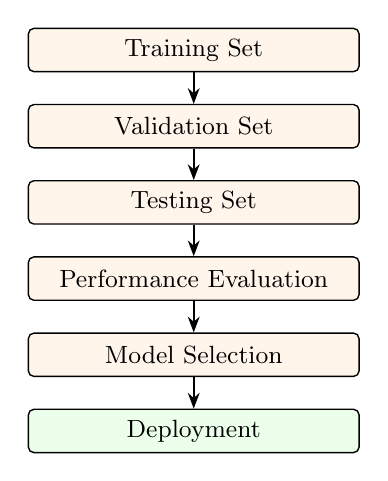
\begin{tikzpicture}[
    font=\small,
    node distance=0mm,
    field/.style={draw, rounded corners=2pt, fill=orange!8, minimum width=4.2cm, minimum height=0.55cm, align=center, line width=0.5pt}
]
\node[field] (train) {Training Set};
\node[field, below=4mm of train] (valset) {Validation Set};
\node[field, below=4mm of valset] (test) {Testing Set};
\node[field, below=4mm of test] (perf) {Performance Evaluation};
\node[field, below=4mm of perf] (sel) {Model Selection};
\node[field, below=4mm of sel, fill=green!8] (dep) {Deployment};

\foreach \a/\b in {train/valset, valset/test, test/perf, perf/sel, sel/dep}
  \draw[-{Stealth[length=2mm]}, line width=0.6pt] (\a.south) -- (\b.north);
\end{tikzpicture}
\caption{Typical model-development workflow, from training, validation, and testing splits through performance evaluation and model selection to deployment.}
\label{fig:model-development}
\end{figure}

\begin{engnote}
Participant-level separation should be maintained between training and testing sets to reduce data leakage.
\end{engnote}

\subsection{Performance Metrics}
\label{sec:performance-metrics}

Models should be evaluated using metrics appropriate to the task, such as: accuracy; precision; recall; F1 score; ROC-AUC (for classification); and the confusion matrix.

\begin{requirementbox}
Confidence intervals should be reported where possible.
\end{requirementbox}

\subsection{Prediction Output}
\label{sec:prediction-output}

The system should output: a predicted class or score; a confidence estimate; and data-quality indicators.

\begin{warningbox}
Predictions must not be presented as medical diagnoses.
\end{warningbox}

\subsection{Safety \& Clinical Scope}
\label{sec:safety-clinical-scope}

\begin{warningbox}
PSYCON should be described as: a research prototype; a screening/research support tool; \textbf{not} a diagnostic device; and \textbf{not} a replacement for licensed mental health professionals. This distinction is important for research competitions and ethical review.
\end{warningbox}

\subsection{Privacy}
\label{sec:privacy-ch7}

Recommended practices: encrypt transmitted data; use anonymized participant IDs; restrict access to research data; and obtain informed consent before collecting physiological or audio data.

\subsection{Model Updating}
\label{sec:model-updating}

\Cref{fig:model-updating} shows the recommended model-update lifecycle.

\begin{figure}[H]
\centering
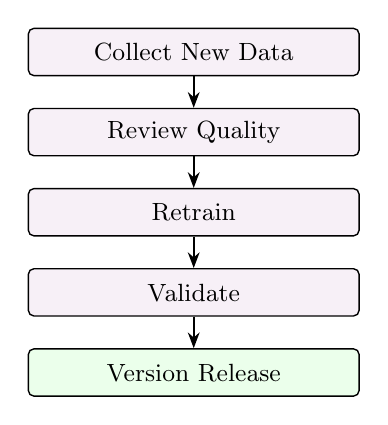
\begin{tikzpicture}[
    font=\small,
    node distance=0mm,
    field/.style={draw, rounded corners=2pt, fill=violet!6, minimum width=4.2cm, minimum height=0.6cm, align=center, line width=0.5pt}
]
\node[field] (new) {Collect New Data};
\node[field, below=4mm of new] (review) {Review Quality};
\node[field, below=4mm of review] (retrain) {Retrain};
\node[field, below=4mm of retrain] (validate) {Validate};
\node[field, below=4mm of validate, fill=green!8] (release) {Version Release};

\foreach \a/\b in {new/review, review/retrain, retrain/validate, validate/release}
  \draw[-{Stealth[length=2mm]}, line width=0.6pt] (\a.south) -- (\b.north);
\end{tikzpicture}
\caption{Recommended model-update lifecycle: collect new data, review quality, retrain, validate, and release a new version.}
\label{fig:model-updating}
\end{figure}

\begin{designnote}
Version numbers should be maintained for both datasets and models.
\end{designnote}

\subsection{AI Validation Checklist}
\label{sec:ai-validation-checklist}

\begin{requirementbox}
\textbf{Before deployment, the following must be verified:}
\begin{itemize}
    \item Sensor synchronization verified.
    \item Audio synchronization verified.
    \item Missing-data handling implemented.
    \item Feature extraction validated.
    \item Model evaluated on unseen data.
    \item Confidence outputs verified.
    \item False-positive/false-negative analysis completed.
    \item Documentation completed.
\end{itemize}
\end{requirementbox}

\subsection{Risks}
\label{sec:risks-ch7}

\begin{observationbox}
\textbf{Potential technical risks:}
\begin{itemize}
    \item Motion artifacts affecting physiological signals.
    \item Environmental noise degrading speech quality.
    \item Missing packets.
    \item Sensor contact loss.
    \item Battery-related interruptions.
    \item Dataset imbalance.
    \item Model overfitting.
    \item Domain shift between training and real-world users.
\end{itemize}
\end{observationbox}

\begin{futureworkbox}
How each risk is mitigated should be documented as part of the AI system's risk register.
\end{futureworkbox}

\subsection{Deliverables}
\label{sec:deliverables-ch7}

The final AI package should include: a data collection protocol; a dataset description; feature documentation; the model architecture; the training procedure; the validation methodology; performance metrics; version history; ethical considerations; and user documentation.

\subsection{Chapter Status}
\label{sec:ch7-status}

\begin{validationbox}
\textbf{Completed for this chapter:}
\begin{itemize}
    \item AI architecture
    \item Data pipeline
    \item Feature engineering overview
    \item Backend workflow
    \item Database design
    \item Model development process
    \item Validation strategy
    \item Privacy and ethics
    \item Risk assessment
    \item Deliverables
\end{itemize}
\end{validationbox}


% ============================================================
% CHAPTER 8
% ============================================================
% ============================================================
% Chapter 8 — System Integration, Verification, Validation & Deployment
% Source: PSYCON Engineering Design Document, Vol. 1, Ch. 8
% ============================================================
\section{System Integration, Verification, Validation, and Deployment}
\label{sec:integration-verification}

\subsection{System Integration Strategy}
\label{sec:integration-strategy}

Integration occurs in five stages, illustrated in \Cref{fig:integration-stages}. Every stage must pass before proceeding to the next.

\begin{figure}[H]
\centering
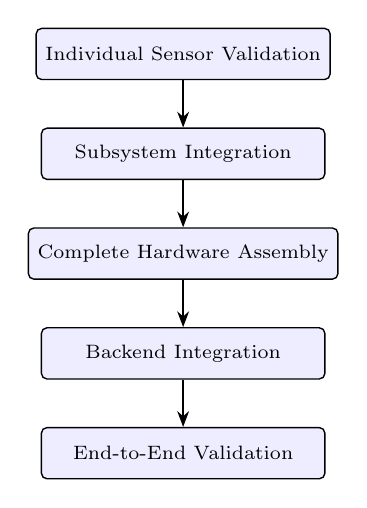
\begin{tikzpicture}[
    font=\scriptsize,
    node distance=0mm,
    field/.style={draw, rounded corners=2pt, fill=blue!7, minimum width=3.6cm, minimum height=0.65cm, align=center, line width=0.5pt}
]
\node[field] (s1) {Individual Sensor Validation};
\node[field, below=6mm of s1] (s2) {Subsystem Integration};
\node[field, below=6mm of s2] (s3) {Complete Hardware Assembly};
\node[field, below=6mm of s3] (s4) {Backend Integration};
\node[field, below=6mm of s4] (s5) {End-to-End Validation};

\draw[-{Stealth[length=2mm]}, line width=0.6pt] (s1.south) -- (s2.north);
\draw[-{Stealth[length=2mm]}, line width=0.6pt] (s2.south) -- (s3.north);
\draw[-{Stealth[length=2mm]}, line width=0.6pt] (s3.south) -- (s4.north);
\draw[-{Stealth[length=2mm]}, line width=0.6pt] (s4.south) -- (s5.north);
\end{tikzpicture}
\caption{Five-stage PSYCON integration strategy, from individual sensor validation through to end-to-end validation.}
\label{fig:integration-stages}
\end{figure}

\subsection{Stage 1 --- Individual Sensor Validation}
\label{sec:stage1-sensor-validation}

Each module is tested independently before integration. \Cref{tab:sensor-validation} summarizes the verification checks and acceptance criteria for each sensor.

\begin{table*}[t]
\centering
\caption{Stage 1 individual sensor validation: verification checks and acceptance criteria.}
\label{tab:sensor-validation}
\small
\begin{tabularx}{\textwidth}{@{}l Y Y@{}}
\toprule
\textbf{Sensor} & \textbf{Verification Checks} & \textbf{Acceptance Criteria} \\
\midrule
MAX30102 & I\textsuperscript{2}C communication; raw RED and IR readings; finger detection; stable waveform; no communication errors & Device detected at \texttt{0x57}; stable signal; no bus failures \\
MPU6050 & Accelerometer; gyroscope; temperature register; axis orientation & Address \texttt{0x68}; stable readings at rest; motion reflected correctly \\
MCP9808 & Ambient temperature; stable readings; repeatability & Address \texttt{0x18}; no sudden fluctuations \\
ADS1115 & Address detection; all four channels readable; stable ADC values & Address \texttt{0x48}; no random saturation \\
TEMT6000 & Analog response to light; dark vs. bright environments & Smooth output variation \\
INMP441 & Audio recording; no clipping; correct I\textsuperscript{2}S configuration; acceptable noise floor & Clean recordings; no DMA overruns \\
\bottomrule
\end{tabularx}
\end{table*}

\subsection{Stage 2 --- I\texorpdfstring{\textsuperscript{2}}{2}C Bus Validation}
\label{sec:stage2-i2c-validation}

An I\textsuperscript{2}C scanner is run across the Wrist Module bus. The expected devices and addresses match those previously listed in \Cref{tab:i2c-addresses}.

\begin{checklist}
    \item All devices detected.
    \item No duplicate addresses.
    \item No intermittent failures.
\end{checklist}

\subsection{Stage 3 --- Integrated Wrist Module}
\label{sec:stage3-wrist-integration}

All wrist sensors are run simultaneously while monitoring bus stability, sampling consistency, CPU utilization, memory usage, and timing accuracy.

\begin{checklist}
    \item Continuous operation without crashes.
    \item Stable timestamps.
    \item No sensor starvation.
\end{checklist}

\subsection{Stage 4 --- Integrated Audio Module}
\label{sec:stage4-audio-integration}

Verification covers continuous microphone capture, ambient light acquisition, and concurrent wireless communication.

\begin{checklist}
    \item No dropped audio buffers.
    \item Stable light sensor readings.
\end{checklist}

\subsection{Stage 5 --- Full System Integration}
\label{sec:stage5-full-integration}

Both modules operate together, with verification of time synchronization, data transmission, backend reception, and session management.

\begin{checklist}
    \item Complete synchronized datasets.
    \item No packet corruption.
\end{checklist}

\subsection{Functional Testing}
\label{sec:functional-testing}

Functional testing confirms that the system can:
\begin{checklist}
    \item Boot successfully.
    \item Detect all sensors.
    \item Acquire data.
    \item Timestamp correctly.
    \item Transmit data.
    \item Recover from temporary communication loss.
    \item Shut down safely.
\end{checklist}

\subsection{Stress Testing}
\label{sec:stress-testing}

\textbf{Tests conducted.}
\begin{itemize}
    \item 1-hour continuous operation.
    \item Extended operation (target duration based on battery capacity).
    \item Rapid reboot cycles.
    \item Repeated connection/disconnection tests.
    \item Continuous wireless transmission.
\end{itemize}

\textbf{Monitored quantities.}
\begin{itemize}
    \item Temperature.
    \item Memory usage.
    \item Packet loss.
    \item Unexpected resets.
\end{itemize}

\subsection{Power Validation}
\label{sec:power-validation}

\textbf{Verification.}
\begin{itemize}
    \item Battery charging.
    \item Battery discharge.
    \item Low-battery detection.
    \item Brownout handling.
    \item Controlled shutdown.
\end{itemize}

\textbf{Recorded quantities.}
\begin{itemize}
    \item Battery voltage.
    \item Runtime.
    \item Charging time.
    \item Device temperature.
\end{itemize}

\subsection{Sensor Calibration}
\label{sec:sensor-calibration}

Calibration procedures are documented for MAX30102, GSR, MCP9808, TEMT6000, and MPU6050. Each calibration record should include:
\begin{itemize}
    \item Calibration date.
    \item Firmware version.
    \item Calibration method.
    \item Environmental conditions.
\end{itemize}

\subsection{Software Validation}
\label{sec:software-validation}

\begin{checklist}
    \item Firmware boots correctly.
    \item Sensor drivers initialize.
    \item Communication stack functions.
    \item Logging system operates.
    \item Error recovery works.
\end{checklist}

\subsection{AI Validation}
\label{sec:ai-validation-ch8}

\begin{checklist}
    \item Feature extraction.
    \item Timestamp synchronization.
    \item Inference pipeline.
    \item Model confidence reporting.
    \item Handling of missing or corrupted data.
\end{checklist}

\subsection{Documentation Package}
\label{sec:documentation-package}

The complete documentation package should include:
\begin{checklist}
    \item Bill of Materials (BOM).
    \item Wiring diagrams.
    \item GPIO map.
    \item Power tree.
    \item Firmware architecture.
    \item AI architecture.
    \item Testing reports.
    \item Calibration records.
    \item Risk assessment.
    \item User manual.
    \item Assembly guide.
    \item Version history.
\end{checklist}

\subsection{Competition Readiness Checklist}
\label{sec:competition-readiness}

\begin{requirementbox}
\textbf{Before submission:}
\begin{checklist}
    \item Hardware fully assembled.
    \item Firmware stable.
    \item AI pipeline validated.
    \item Documentation complete.
    \item Safety review completed.
    \item Demonstration rehearsed.
    \item Backup firmware available.
    \item Backup hardware available (where practical).
\end{checklist}
\end{requirementbox}

\subsection{Known Remaining Risks}
\label{sec:known-remaining-risks-ch8}

\begin{observationbox}
\textbf{Current engineering risks include:}
\begin{itemize}
    \item GSR analog front-end refinement.
    \item Battery runtime limitations.
    \item Wireless reliability in congested environments.
    \item Motion artifacts affecting physiological signals.
    \item Audio quality in noisy environments.
    \item Long-term sensor stability.
\end{itemize}
Each risk should have a documented mitigation strategy.
\end{observationbox}

\subsection{Final Deliverables}
\label{sec:final-deliverables}

The complete PSYCON package should contain:
\begin{itemize}
    \item Hardware prototype.
    \item Embedded firmware.
    \item AI models.
    \item Backend software.
    \item Mobile/web interface (if applicable).
    \item Technical documentation.
    \item Validation and testing reports.
    \item User and maintenance guides.
    \item Safety and ethics documentation.
    \item Research report.
\end{itemize}

\subsection{Volume 1 Summary}
\label{sec:volume1-summary}

\begin{validationbox}
\textbf{This concludes the core engineering design document, covering:}
\begin{itemize}
    \item Project overview
    \item Hardware architecture
    \item Electrical design
    \item Firmware architecture
    \item AI pipeline
    \item System integration
    \item Verification and validation
\end{itemize}
\end{validationbox}


\clearpage
\part{Volume 2: Manufacturing, Mechanical Design \& Future Roadmap}

% ============================================================
% CHAPTER 9
% ============================================================
% ============================================================
% Chapter 9 — Manufacturing, PCB Design & Mechanical Engineering
% Source: PSYCON Engineering Design Document, Vol. 2, Ch. 9
% ============================================================
\section{Manufacturing, PCB Design, and Mechanical Engineering}
\label{sec:manufacturing}

\subsection{Manufacturing Philosophy}
\label{sec:manufacturing-philosophy}

PSYCON is designed as a research prototype with a clear migration path, shown in \Cref{fig:manufacturing-path}. The current implementation emphasizes rapid prototyping, validation, and documentation before hardware miniaturization.

\begin{figure}[H]
\centering
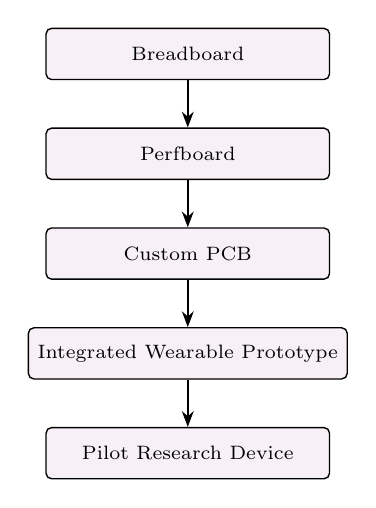
\begin{tikzpicture}[
    font=\scriptsize,
    node distance=0mm,
    field/.style={draw, rounded corners=2pt, fill=violet!6, minimum width=3.6cm, minimum height=0.65cm, align=center, line width=0.5pt}
]
\node[field] (s1) {Breadboard};
\node[field, below=6mm of s1] (s2) {Perfboard};
\node[field, below=6mm of s2] (s3) {Custom PCB};
\node[field, below=6mm of s3] (s4) {Integrated Wearable Prototype};
\node[field, below=6mm of s4] (s5) {Pilot Research Device};

\draw[-{Stealth[length=2mm]}, line width=0.6pt] (s1.south) -- (s2.north);
\draw[-{Stealth[length=2mm]}, line width=0.6pt] (s2.south) -- (s3.north);
\draw[-{Stealth[length=2mm]}, line width=0.6pt] (s3.south) -- (s4.north);
\draw[-{Stealth[length=2mm]}, line width=0.6pt] (s4.south) -- (s5.north);
\end{tikzpicture}
\caption{PSYCON manufacturing migration path, from breadboard prototyping through to a pilot research device.}
\label{fig:manufacturing-path}
\end{figure}

\subsection{PCB Design Goals}
\label{sec:pcb-design-goals}

The custom PCB should:
\begin{itemize}
    \item Reduce wiring complexity.
    \item Improve signal integrity.
    \item Lower power consumption.
    \item Reduce mechanical failure points.
    \item Simplify assembly.
    \item Improve repeatability across multiple units.
\end{itemize}

\subsection{PCB Architecture}
\label{sec:pcb-architecture}

\Cref{tab:pcb-architecture} summarizes which components are integrated on the Wrist PCB versus the Audio PCB.

\begin{table*}[t]
\centering
\caption{PCB architecture: component allocation between the Wrist PCB and Audio PCB.}
\label{tab:pcb-architecture}
\small
\begin{tabularx}{\textwidth}{@{}Y c c@{}}
\toprule
\textbf{Component} & \textbf{Wrist PCB} & \textbf{Audio PCB} \\
\midrule
ESP32 & \checkmark & \checkmark \\
MAX30102 & \checkmark & --- \\
ADS1115 & \checkmark & --- \\
MCP9808 & \checkmark & --- \\
MPU6050 & \checkmark & --- \\
GSR analog front-end & \checkmark & --- \\
INMP441 & --- & \checkmark \\
TEMT6000 & --- & \checkmark \\
Battery connector & \checkmark & \checkmark \\
Charging interface & \checkmark & \checkmark \\
Programming header & \checkmark & \checkmark \\
Power regulation & \checkmark & --- \\
Status LEDs & --- & \checkmark \\
\bottomrule
\end{tabularx}
\end{table*}

\subsection{Mechanical Layout}
\label{sec:mechanical-layout}

\Cref{fig:mechanical-layout} shows the suggested mechanical stack-up for both modules.

\begin{figure*}[t]
\centering
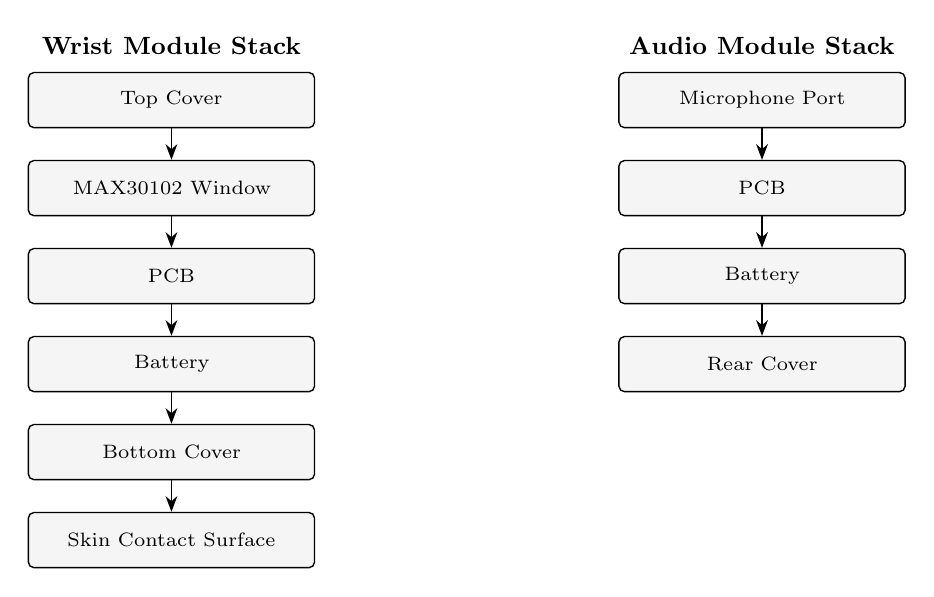
\begin{tikzpicture}[
    font=\scriptsize,
    layer/.style={draw, rounded corners=2pt, text width=3.4cm, minimum height=0.7cm, align=center, line width=0.5pt, fill=gray!8},
    arrow/.style={-{Stealth[length=2mm]}, line width=0.6pt}
]
% Wrist Module stack
\node[layer] (w1) at (0,5.4) {Top Cover};
\node[layer, below=4mm of w1] (w2) {MAX30102 Window};
\node[layer, below=4mm of w2] (w3) {PCB};
\node[layer, below=4mm of w3] (w4) {Battery};
\node[layer, below=4mm of w4] (w5) {Bottom Cover};
\node[layer, below=4mm of w5] (w6) {Skin Contact Surface};

\draw[arrow] (w1.south) -- (w2.north);
\draw[arrow] (w2.south) -- (w3.north);
\draw[arrow] (w3.south) -- (w4.north);
\draw[arrow] (w4.south) -- (w5.north);
\draw[arrow] (w5.south) -- (w6.north);

\node[above=1mm of w1, font=\bfseries\small] {Wrist Module Stack};

% Audio Module stack
\node[layer] (a1) at (7.5,5.4) {Microphone Port};
\node[layer, below=4mm of a1] (a2) {PCB};
\node[layer, below=4mm of a2] (a3) {Battery};
\node[layer, below=4mm of a3] (a4) {Rear Cover};

\draw[arrow] (a1.south) -- (a2.north);
\draw[arrow] (a2.south) -- (a3.north);
\draw[arrow] (a3.south) -- (a4.north);

\node[above=1mm of a1, font=\bfseries\small] {Audio Module Stack};

\end{tikzpicture}
\caption{Suggested mechanical stack-up for the Wrist Module (top cover through skin-contact surface) and Audio Module (microphone port through rear cover).}
\label{fig:mechanical-layout}
\end{figure*}

\textbf{Wrist Module.} The optical sensor should remain flush against the skin, while electronics are isolated from direct skin contact.

\textbf{Audio Module.} The microphone opening should remain unobstructed and protected from dust.

\subsection{Enclosure Requirements}
\label{sec:enclosure-requirements}

\begin{itemize}
    \item Lightweight.
    \item Rounded edges.
    \item Sweat resistant.
    \item Battery securely retained.
    \item Accessible USB charging port.
    \item Reset/programming access.
    \item Ventilation where required.
    \item Strain relief for any external wiring.
\end{itemize}

\subsection{Assembly Process}
\label{sec:assembly-process}

\begin{enumerate}
    \item Inspect all PCBs.
    \item Verify battery polarity.
    \item Assemble power system.
    \item Program ESP32 firmware.
    \item Test each sensor individually.
    \item Integrate all modules.
    \item Perform system-level verification.
    \item Close enclosure.
    \item Final functional test.
\end{enumerate}

\subsection{Quality Control Checklist}
\label{sec:qc-checklist}

\textbf{Before final assembly:}
\begin{checklist}
    \item No solder bridges.
    \item Correct component orientation.
    \item Secure connectors.
    \item Proper insulation.
    \item Stable power rails.
    \item All sensors detected.
    \item Firmware version recorded.
\end{checklist}

\subsection{Maintenance}
\label{sec:maintenance}

\textbf{Recommended periodic checks:}
\begin{itemize}
    \item Battery health.
    \item Connector wear.
    \item Sensor cleanliness.
    \item Enclosure integrity.
    \item Firmware updates.
    \item Calibration verification.
\end{itemize}

\subsection{Reliability Considerations}
\label{sec:reliability-considerations}

\begin{observationbox}
\textbf{Potential failure modes:}
\begin{itemize}
    \item Battery degradation.
    \item Loose connectors.
    \item Sensor contamination.
    \item Wire fatigue.
    \item Moisture ingress.
    \item Firmware corruption.
    \item Electrostatic discharge (ESD).
\end{itemize}
Documented mitigation should be provided for each failure mode.
\end{observationbox}

\subsection{Future Improvements}
\label{sec:future-improvements-ch9}

\begin{futureworkbox}
\textbf{Potential upgrades:}
\begin{itemize}
    \item Custom low-power PCB.
    \item Dedicated medical-grade GSR analog front-end.
    \item Lower-power MCU variants.
    \item Larger-capacity battery with improved power management.
    \item Secure data encryption hardware.
    \item OTA firmware updates.
    \item Additional physiological sensors (only after validating clinical usefulness).
    \item Improved enclosure with waterproofing.
\end{itemize}
\end{futureworkbox}

\subsection{Scalability}
\label{sec:scalability-ch9}

Future versions may support:
\begin{itemize}
    \item Multiple wearable form factors.
    \item Cloud synchronization.
    \item Long-duration monitoring.
    \item Clinical research dashboards.
    \item Multi-user study management.
    \item Automated firmware update system.
\end{itemize}

\subsection{Final Manufacturing Deliverables}
\label{sec:final-manufacturing-deliverables}

\begin{checklist}
    \item Complete Bill of Materials (BOM).
    \item PCB design files.
    \item Schematic diagrams.
    \item Assembly drawings.
    \item Wiring diagrams.
    \item Mechanical CAD files.
    \item Enclosure STL files.
    \item Firmware source code.
    \item AI model documentation.
    \item Test reports.
    \item Validation records.
    \item User documentation.
    \item Risk assessment.
\end{checklist}

\subsection{Volume 2 Status}
\label{sec:volume2-status}

\begin{validationbox}
\textbf{Completed for this chapter:}
\begin{itemize}
    \item Manufacturing strategy
    \item PCB migration plan
    \item Mechanical architecture
    \item Enclosure requirements
    \item Assembly workflow
    \item Quality control
    \item Maintenance plan
    \item Reliability considerations
    \item Future roadmap
\end{itemize}
\end{validationbox}


\clearpage
\part{Volume 3: Reference Documentation}

% ============================================================
% CHAPTER 10
% ============================================================
% ============================================================
% Chapter 10 — Complete Bill of Materials (BOM)
% Source: PSYCON Engineering Design Document, Vol. 3, Ch. 10
% ============================================================
\section{Complete Bill of Materials}
\label{sec:complete-bom}

\subsection{Wrist Module BOM}
\label{sec:wrist-bom}

\Cref{tab:wrist-bom} lists the complete bill of materials for the Wrist Module.

\begin{table*}[t]
\centering
\caption{Wrist Module bill of materials.}
\label{tab:wrist-bom}
\small
\begin{tabularx}{\textwidth}{@{}l Y Y@{}}
\toprule
\textbf{Qty.} & \textbf{Component} & \textbf{Purpose} \\
\midrule
1 & ESP32 DevKit V1 (30-pin) & Main controller \\
1 & MAX30102 & Heart rate \& PPG \\
1 & ADS1115 & 16-bit ADC for GSR \\
1 & MPU6050 & Motion sensing \\
1 & MCP9808 & Temperature sensing \\
1 pair & GSR electrodes & Skin conductance measurement \\
1 & TP4056 USB-C charger (protected) & Battery charging \\
2 & 500\,mAh LiPo cells (parallel) & Power source \\
1 & Power switch & Main power \\
1 & JST connector & Battery connection \\
Several & Male/female headers & Module connections \\
Several & Hook-up wires & Wiring \\
1 & Wrist enclosure & Housing \\
\bottomrule
\end{tabularx}
\end{table*}

\subsection{Audio Module BOM}
\label{sec:audio-bom}

\Cref{tab:audio-bom} lists the complete bill of materials for the Audio Module.

\begin{table*}[t]
\centering
\caption{Audio Module bill of materials.}
\label{tab:audio-bom}
\small
\begin{tabularx}{\textwidth}{@{}l Y Y@{}}
\toprule
\textbf{Qty.} & \textbf{Component} & \textbf{Purpose} \\
\midrule
1 & ESP32 DevKit V1 (30-pin) & Main controller \\
1 & INMP441 & I\textsuperscript{2}S microphone \\
1 & TEMT6000 & Ambient light sensor \\
1 & TP4056 USB-C charger (protected) & Battery charging \\
1 & 500\,mAh LiPo cell & Power source \\
1 & Power switch & Main power \\
1 & JST connector & Battery connection \\
Several & Hook-up wires & Wiring \\
1 & Enclosure & Housing \\
\bottomrule
\end{tabularx}
\end{table*}

\subsection{Shared Tools}
\label{sec:shared-tools}

\begin{itemize}
    \item Breadboard
    \item Soldering iron
    \item Solder wire
    \item Flux
    \item Heat-shrink tubing
    \item USB-C cable
    \item ESP32 programming cable
    \item Small screwdrivers
    \item Tweezers
    \item Hot glue/Kapton tape for strain relief
\end{itemize}

\subsection{Electrical Specifications}
\label{sec:bom-electrical-specs}

\textbf{Logic voltage.} ESP32 GPIO: 3.3\,V. All digital interfaces: 3.3\,V.

\textbf{Battery.} Nominal: 3.7\,V. Fully charged: 4.2\,V. Recommended cutoff: $\approx$3.2--3.3\,V under light load.

\textbf{Communication.} I\textsuperscript{2}C; I\textsuperscript{2}S; Wi-Fi; BLE.

\subsection{Week 7 Cost Status}

The BOM fixes functional quantities but does not identify every purchased manufacturer part number or a dated price. The candidate release therefore includes a budget template rather than an invented total. Final costing must record vendor, part number, quantity, unit price, shipping, tax, currency, purchase date, and invoice reference. Reusable tools must remain separate from per-prototype cost.


% ============================================================
% CHAPTER 11
% ============================================================
% ============================================================
% Chapter 11 — Complete GPIO Assignment
% Source: PSYCON Engineering Design Document, Vol. 3, Ch. 11
% ============================================================
\section{Complete GPIO Assignment}
\label{sec:complete-gpio}

\subsection{Wrist Module}
\label{sec:complete-gpio-wrist}

\Cref{tab:wrist-gpio-ref} lists the complete GPIO assignment for the Wrist Module, and \Cref{tab:i2c-addresses-ref} lists the corresponding I\textsuperscript{2}C device addresses.

\begin{table}[H]
\centering
\caption{Wrist Module GPIO assignment (reference summary).}
\label{tab:wrist-gpio-ref}
\small
\begin{tabularx}{\columnwidth}{@{}l Y@{}}
\toprule
\textbf{ESP32 Pin} & \textbf{Device} \\
\midrule
GPIO21 & I\textsuperscript{2}C SDA \\
GPIO22 & I\textsuperscript{2}C SCL \\
GPIO34 & GSR (ADS1115 input interface) \\
GPIO35 & Battery monitoring (if used) \\
3V3 & Sensors \\
GND & Common ground \\
\bottomrule
\end{tabularx}
\end{table}

\begin{table}[H]
\centering
\caption{I\textsuperscript{2}C device addresses (reference summary).}
\label{tab:i2c-addresses-ref}
\small
\begin{tabularx}{\columnwidth}{@{}Y l@{}}
\toprule
\textbf{Device} & \textbf{Address} \\
\midrule
MCP9808 & \texttt{0x18} \\
ADS1115 & \texttt{0x48} \\
MAX30102 & \texttt{0x57} \\
MPU6050 & \texttt{0x68} \\
\bottomrule
\end{tabularx}
\end{table}

\subsection{Audio Module}
\label{sec:complete-gpio-audio}

\Cref{tab:audio-gpio-ref} lists the complete GPIO assignment for the Audio Module.

\begin{table}[H]
\centering
\caption{Audio Module GPIO assignment (reference summary).}
\label{tab:audio-gpio-ref}
\small
\begin{tabularx}{\columnwidth}{@{}l Y@{}}
\toprule
\textbf{ESP32 Pin} & \textbf{Device} \\
\midrule
GPIO21 & I\textsuperscript{2}C SDA (if required) \\
GPIO22 & I\textsuperscript{2}C SCL (if required) \\
GPIO25 & I\textsuperscript{2}S WS \\
GPIO26 & I\textsuperscript{2}S SCK \\
GPIO33 & I\textsuperscript{2}S SD \\
GPIO32 & TEMT6000 analog input \\
3V3 & Sensor power \\
GND & Ground \\
\bottomrule
\end{tabularx}
\end{table}


% ============================================================
% CHAPTER 12
% ============================================================
% ============================================================
% Chapter 12 — Wiring Rules
% Source: PSYCON Engineering Design Document, Vol. 3, Ch. 12
% ============================================================
\section{Wiring Rules}
\label{sec:wiring-rules}

\subsection{Always}
\label{sec:wiring-always}

\begin{itemize}
    \item Share one common ground.
    \item Keep I\textsuperscript{2}C wires short.
    \item Keep microphone traces away from power lines.
    \item Separate analog GSR wiring from digital signals.
    \item Twist long GSR leads if possible.
    \item Secure battery wiring to prevent movement.
\end{itemize}

\subsection{Avoid}
\label{sec:wiring-avoid}

\begin{warningbox}
\begin{itemize}
    \item 5\,V directly on ESP32 GPIOs.
    \item Charging while electrodes are attached.
    \item Long unshielded microphone wires.
    \item Loose JST connectors.
\end{itemize}
\end{warningbox}


% ============================================================
% CHAPTER 13
% ============================================================
% ============================================================
% Chapter 13 — Calibration Summary
% Source: PSYCON Engineering Design Document, Vol. 3, Ch. 13
% ============================================================
\section{Calibration Summary}
\label{sec:calibration-summary}

For each sensor, the following should be documented:
\begin{itemize}
    \item Calibration date
    \item Firmware version
    \item Environmental conditions
    \item Test operator
    \item Calibration method
    \item Results
\end{itemize}

\begin{requirementbox}
Recalibration is required after hardware modifications or sensor replacement.
\end{requirementbox}


% ============================================================
% CHAPTER 14
% ============================================================
% ============================================================
% Chapter 14 — Test Log Template
% Source: PSYCON Engineering Design Document, Vol. 3, Ch. 14
% ============================================================
\section{Test Log Template}
\label{sec:test-log-template}

\Cref{tab:test-log-fields} lists the fields to be recorded for every build.

\begin{table}[H]
\centering
\caption{Test log template fields.}
\label{tab:test-log-fields}
\small
\begin{tabularx}{\columnwidth}{@{}Y@{}}
\toprule
\textbf{Field} \\
\midrule
Hardware revision \\
Firmware version \\
Date \\
Tester \\
Sensor initialization results \\
I\textsuperscript{2}C scan results \\
Battery voltage \\
Runtime \\
Charging time \\
Communication status \\
Notes and corrective actions \\
\bottomrule
\end{tabularx}
\end{table}


% ============================================================
% CHAPTER 15
% ============================================================
% ============================================================
% Chapter 15 — Risk Register
% Source: PSYCON Engineering Design Document, Vol. 3, Ch. 15
% ============================================================
\section{Risk Register}
\label{sec:risk-register}

\Cref{tab:risk-register} consolidates the project's known risks, their impact level, and the corresponding mitigation strategy.

\begin{table*}[t]
\centering
\caption{PSYCON risk register.}
\label{tab:risk-register}
\small
\begin{tabularx}{\textwidth}{@{}Y c Y@{}}
\toprule
\textbf{Risk} & \textbf{Impact} & \textbf{Mitigation} \\
\midrule
Battery depletion & \highriskTag & Low-battery detection \& controlled shutdown \\
Sensor disconnect & \medriskTag & Startup/self-test \& continuous monitoring \\
I\textsuperscript{2}C communication failure & \medriskTag & Retry and error logging \\
Motion artifacts & \highriskTag & Filtering and quality metrics \\
Audio noise & \medriskTag & Mechanical isolation and preprocessing \\
GSR electrode contact loss & \highriskTag & Contact-quality checks and proper placement \\
Firmware crash & \highriskTag & Watchdog timer and restart \\
Wireless interruption & \medriskTag & Packet buffering and retry \\
Data corruption & \highriskTag & Checksums and sequence numbers \\
\bottomrule
\end{tabularx}
\end{table*}


% ============================================================
% CHAPTER 16
% ============================================================
% ============================================================
% Chapter 16 — Project Deliverables
% Source: PSYCON Engineering Design Document, Vol. 3, Ch. 16
% ============================================================
\section{Project Deliverables}
\label{sec:project-deliverables}

The final PSYCON package should include:
\begin{checklist}
    \item Hardware prototype
    \item Firmware source code
    \item Wiring diagrams
    \item Bill of Materials (BOM)
    \item Schematics
    \item AI documentation
    \item Testing reports
    \item Validation reports
    \item Risk assessment
    \item User manual
    \item Assembly guide
    \item Maintenance guide
    \item Version history
    \item Competition report
    \item Demonstration material
\end{checklist}

\subsection{Week 7 Candidate Package}

The repository now contains a user manual, assembly and maintenance guide, competition package, demonstration runbook, official reference index, model card, dataset card, final evidence matrix, release checklist, budget template, demonstration-record template, and a deterministic archive builder. The builder records versions, the source commit, tracked-change state, file sizes, SHA-256 hashes, exclusions, and release blockers.

The package remains \texttt{psycon-1.0.0-rc1} with candidate status. Hardware and PCB freeze, complete firmware, physical validation, the PSYCON study dataset and model, priced BOM, third-person reproduction, and live and recorded demonstrations remain open.

\subsection{Volume 3 Status}
\label{sec:volume3-status}

\begin{validationbox}
\textbf{Completed for this volume:}
\begin{itemize}
    \item Complete BOM
    \item GPIO assignments
    \item Electrical specifications
    \item Wiring rules
    \item Calibration documentation
    \item Test logging template
    \item Risk register
    \item Final deliverables
\end{itemize}
\end{validationbox}


\clearpage
\part{Volume 4: Research Methodology, Ethics \& Competition Documentation}

% ============================================================
% CHAPTER 17
% ============================================================
% ============================================================
% Chapter 17 — Research Methodology
% Source: PSYCON Engineering Design Document, Vol. 4, Ch. 17
% ============================================================
\section{Research Methodology}
\label{sec:research-methodology}

\subsection{Research Objective}
\label{sec:research-objective}

The objective of PSYCON is to investigate whether multimodal physiological and speech-derived features can be combined to estimate indicators relevant to psychological well-being in a research setting. The system is intended as a research and screening prototype, not a diagnostic medical device.

\subsection{Research Questions}
\label{sec:research-questions}

\textbf{Primary questions:}
\begin{itemize}
    \item Can physiological and speech features improve predictive performance compared with either modality alone?
    \item How robust are predictions under different environmental conditions?
    \item How does motion affect signal quality?
    \item What is the minimum recording duration needed for stable feature extraction?
\end{itemize}

\subsection{Study Design}
\label{sec:study-design}

\Cref{fig:study-workflow} shows the suggested end-to-end study workflow.

\begin{figure}[H]
\centering
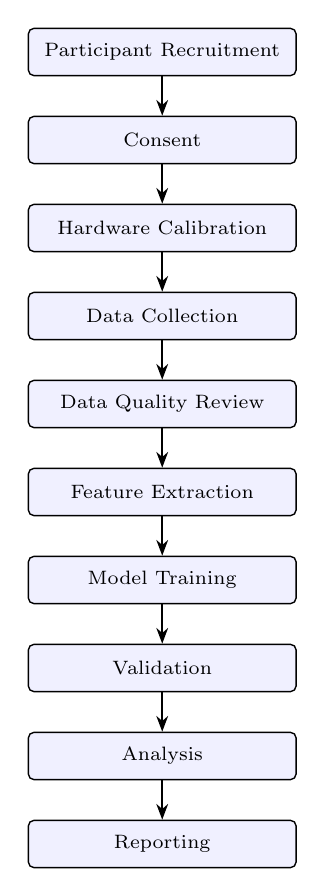
\begin{tikzpicture}[
    font=\scriptsize,
    node distance=0mm,
    field/.style={draw, rounded corners=2pt, fill=blue!6, minimum width=3.4cm, minimum height=0.6cm, align=center, line width=0.5pt}
]
\node[field] (s1) {Participant Recruitment};
\node[field, below=5mm of s1] (s2) {Consent};
\node[field, below=5mm of s2] (s3) {Hardware Calibration};
\node[field, below=5mm of s3] (s4) {Data Collection};
\node[field, below=5mm of s4] (s5) {Data Quality Review};
\node[field, below=5mm of s5] (s6) {Feature Extraction};
\node[field, below=5mm of s6] (s7) {Model Training};
\node[field, below=5mm of s7] (s8) {Validation};
\node[field, below=5mm of s8] (s9) {Analysis};
\node[field, below=5mm of s9] (s10) {Reporting};

\foreach \i/\j in {s1/s2, s2/s3, s3/s4, s4/s5, s5/s6, s6/s7, s7/s8, s8/s9, s9/s10}
  \draw[-{Stealth[length=2mm]}, line width=0.6pt] (\i.south) -- (\j.north);
\end{tikzpicture}
\caption{Suggested end-to-end study workflow, from participant recruitment and consent through data collection, feature extraction, model training and validation, to final analysis and reporting.}
\label{fig:study-workflow}
\end{figure}

\subsection{Participants}
\label{sec:participants}

For each participant, the following should be recorded:
\begin{itemize}
    \item Anonymous participant ID
    \item Age group (if relevant)
    \item Biological sex (optional, if ethically approved)
    \item Recording date/time
    \item Session duration
    \item Environmental conditions
    \item Device firmware version
\end{itemize}

\begin{warningbox}
Avoid collecting personally identifying information unless necessary and approved.
\end{warningbox}

\subsection{Data Collection Protocol}
\label{sec:data-collection-protocol}

For every session:
\begin{enumerate}
    \item Verify hardware operation.
    \item Confirm battery level.
    \item Attach wrist module.
    \item Position audio module.
    \item Start synchronized recording.
    \item Monitor system status.
    \item End recording.
    \item Save data.
    \item Backup data.
    \item Review data quality.
\end{enumerate}

\subsection{Recorded Variables}
\label{sec:recorded-variables}

\Cref{tab:recorded-variables} lists the variables recorded for each session, organized by category.

\begin{table}[H]
\centering
\caption{Recorded variables by category.}
\label{tab:recorded-variables}
\small
\begin{tabularx}{\columnwidth}{@{}l Y@{}}
\toprule
\textbf{Category} & \textbf{Variables} \\
\midrule
Physiological & Heart rate; PPG waveform; GSR; temperature; motion; ambient light; battery status \\
Speech & Audio recording (if consented); extracted acoustic features; extracted language features \\
System & Timestamp; session ID; firmware version; sensor status; error logs \\
\bottomrule
\end{tabularx}
\end{table}

\subsection{Inclusion Criteria}
\label{sec:inclusion-criteria}

\textbf{Example criteria:}
\begin{itemize}
    \item Adult participants (or appropriate guardian consent for minors).
    \item Ability to provide informed consent.
    \item Ability to wear the device comfortably.
\end{itemize}

\subsection{Exclusion Criteria}
\label{sec:exclusion-criteria}

\textbf{Example criteria:}
\begin{itemize}
    \item Damaged skin at electrode location.
    \item Implanted medical devices, if required by the safety review.
    \item Participants unwilling to consent to physiological or audio recording.
\end{itemize}


% ============================================================
% CHAPTER 18
% ============================================================
% ============================================================
% Chapter 18 — Data Management
% Source: PSYCON Engineering Design Document, Vol. 4, Ch. 18
% ============================================================
\section{Data Management}
\label{sec:data-management}

\subsection{Storage}
\label{sec:data-storage}

The following should be maintained:
\begin{itemize}
    \item Raw sensor files
    \item Processed feature files
    \item Metadata
    \item Model outputs
    \item Logs
\end{itemize}

\begin{engnote}
Use regular backups and version control.
\end{engnote}

\subsection{File Structure}
\label{sec:data-file-structure}

\Cref{lst:data-file-structure} shows the recommended top-level data repository layout.

\begin{lstlisting}[caption={Recommended PSYCON data repository structure.}, label={lst:data-file-structure}]
/participants
/sessions
  /raw
  /features
/models
/results
/docs
/firmware
\end{lstlisting}

\subsection{Version Control}
\label{sec:data-version-control}

The following should be tracked:
\begin{itemize}
    \item Firmware version
    \item Hardware revision
    \item PCB revision
    \item Dataset version
    \item Model version
    \item Documentation revision
\end{itemize}


% ============================================================
% CHAPTER 19
% ============================================================
% ============================================================
% Chapter 19 — Ethics & Privacy
% Source: PSYCON Engineering Design Document, Vol. 4, Ch. 19
% ============================================================
\section{Ethics and Privacy}
\label{sec:ethics-privacy}

\subsection{Ethical Principles}
\label{sec:ethical-principles}

\begin{itemize}
    \item Voluntary participation.
    \item Informed consent.
    \item Right to withdraw.
    \item Data minimization.
    \item Secure storage.
    \item Limited access.
    \item Transparent reporting.
\end{itemize}

\begin{requirementbox}
If recording speech, clearly explain what is collected, how it is processed, how long it is retained, and who can access it.
\end{requirementbox}

\subsection{Wearer Voice Profile}
\label{sec:wearer-voice-profile-privacy}

Speaker verification is biometric processing and requires consent separate from permission to process the conversation recording. Week~3 supports one local wearer profile created from three quality-checked recordings. Only the normalized averaged voice embedding and non-identifying enrollment metadata may be retained; the source enrollment recordings must be discarded immediately after processing. The profile must be encrypted using an operator-provisioned secret, excluded from logs and API responses, and replaceable or deletable by the operator.

The profile may identify only the enrolled wearer. Other voices remain anonymous recording-local speaker labels, and an uncertain comparison must abstain rather than select the nearest voice. Production deployment additionally requires authenticated access, encrypted transport, audit logging, a documented retention period, and measured false-match and false-rejection rates across the intended languages, microphones, and environments.


% ============================================================
% CHAPTER 20
% ============================================================
% ============================================================
% Chapter 20 — Statistical Analysis Plan
% Source: PSYCON Engineering Design Document, Vol. 4, Ch. 20
% ============================================================
\section{Statistical Analysis Plan}
\label{sec:statistical-analysis-plan}

Potential analyses include:
\begin{itemize}
    \item Descriptive statistics
    \item Correlation analysis
    \item Classification metrics
    \item Cross-validation
    \item Ablation studies (speech only vs.\ physiology only vs.\ combined)
    \item Error analysis
    \item Confusion matrices
    \item ROC curves (where applicable)
\end{itemize}

\begin{observationbox}
Both overall performance and limitations should be reported.
\end{observationbox}

\subsection{Implemented Evaluation Procedure}
\label{sec:implemented-evaluation-procedure}

The Week 5 evaluator creates one deterministic participant-level train, validation, and test assignment and reuses it for physiology-only, speech-only, and combined comparisons. Preprocessing is fitted inside each training pipeline. Logistic regression and random forest are the current candidates, validation F1 selects the candidate, and the chosen pipeline is refitted on the training and validation participants before one held-out test evaluation.

The output contract includes accuracy, precision, recall, F1, ROC-AUC when both classes are present, confusion matrices, false-positive and false-negative counts, grouped cross-validation, participant-level bootstrap confidence intervals, descriptive statistics, feature correlations, prediction and error rows, modality ablations, data-quality coverage, environment and motion slices, and 10, 30, and 60-second duration summaries. External validation rejects participant overlap and incompatible feature columns.

\begin{observationbox}
These procedures are implemented and covered by unit tests, but no Week 5 metric is reported because no completed marksheet and matching PSYCON recording dataset is available. The target definition, primary metric, \texttt{N/O} handling, exclusions, and duration-stability tolerance must be frozen before the test set is opened.
\end{observationbox}


% ============================================================
% CHAPTER 21
% ============================================================
% ============================================================
% Chapter 21 — Competition Documentation
% Source: PSYCON Engineering Design Document, Vol. 4, Ch. 21
% ============================================================
\section{Competition Documentation}
\label{sec:competition-documentation}

The following should be prepared:
\begin{checklist}
    \item Executive summary
    \item Abstract
    \item Problem statement
    \item Innovation overview
    \item Hardware architecture
    \item Software architecture
    \item AI methodology
    \item Testing results
    \item Limitations
    \item Future work
    \item References
    \item Safety statement
    \item Ethics statement
    \item Budget
    \item Timeline
\end{checklist}

The Week 7 competition document supplies each listed section and links the underlying evidence. The budget remains an unpriced template because dated supplier records were not supplied. Testing and AI results distinguish WESAD development evidence from absent PSYCON hardware and participant results. This package supports a software and documentation presentation, not a completed-system claim.


% ============================================================
% CHAPTER 22
% ============================================================
% ============================================================
% Chapter 22 — Demonstration Plan
% Source: PSYCON Engineering Design Document, Vol. 4, Ch. 22
% ============================================================
\section{Demonstration Plan}
\label{sec:demonstration-plan}

A live demonstration should be prepared, showing:
\begin{itemize}
    \item Device startup.
    \item Sensor initialization.
    \item Live physiological acquisition.
    \item Live audio capture (with consent).
    \item Data synchronization.
    \item Backend visualization.
    \item AI inference output.
    \item Consented wearer enrollment and encrypted-profile deletion.
    \item Anonymous speaker timeline, conservative wearer match, and attributed transcript.
    \item Per-speaker speaking rates, pauses, response gaps, overlaps, interruptions, and jitter with unavailable reasons.
    \item Safe shutdown.
\end{itemize}

\begin{requirementbox}
A recorded backup demonstration should also be prepared in case of hardware issues.
\end{requirementbox}

The Week~3 software demonstration uses a consented multilingual recording with at least two speakers, natural pauses, and overlap. It must show that missing model access, missing enrollment, ambiguous identity, and poor-quality speech produce explicit abstention states while acoustic analysis and transcription remain independently usable.


% ============================================================
% CHAPTER 23
% ============================================================
% ============================================================
% Chapter 23 — Project Limitations
% Source: PSYCON Engineering Design Document, Vol. 4, Ch. 23
% ============================================================
\section{Project Limitations}
\label{sec:project-limitations}

Current limitations include:
\begin{itemize}
    \item Prototype hardware rather than custom PCB.
    \item Battery life constrained by ESP32 development boards.
    \item GSR accuracy dependent on analog front-end implementation.
    \item Performance depends on the quality and diversity of training data.
    \item No completed psychologist marksheet dataset has been joined to matching PSYCON wrist and audio sessions.
    \item Week 5 has evaluation software but no empirical multimodal, minimum-duration, or external-validation result.
    \item One Wrist Module measures only one focal wearer in a circle session; center audio cannot provide physiology for the other speakers.
    \item The current audio application can verify one enrolled wearer, while other speakers remain anonymous recording-local clusters and overlap may remain unattributed.
    \item Week 7 can freeze a software and documentation candidate, but absent hardware, study, and demonstration evidence prevents a final release.
\end{itemize}

\begin{warningbox}
Outputs are intended for research support and must not be interpreted as clinical diagnoses.
\end{warningbox}

\subsection{Volume 4 Status}
\label{sec:volume4-status}

\begin{validationbox}
\textbf{Completed as design or implementation documentation for this volume:}
\begin{itemize}
    \item Research methodology
    \item Study protocol
    \item Data management
    \item Ethics and privacy
    \item Statistical analysis plan
    \item Competition documentation
    \item Demonstration plan
    \item Limitations
\end{itemize}
Study execution, participant data, model results, and external validation remain pending and are not implied by this documentation status.
\end{validationbox}


\clearpage
\part{Volume 5: Appendices, Reference Material \& Project Closure}

% ============================================================
% CHAPTER 24
% ============================================================
% ============================================================
% Chapter 24 — Datasheet & Reference Index
% Source: PSYCON Engineering Design Document, Vol. 5, Ch. 24
% ============================================================
\section{Datasheet and Reference Index}
\label{sec:datasheet-reference-index}

The references in \Cref{tab:datasheet-index} should be maintained as part of the project documentation. Official manufacturer datasheets should be used where available.

\begin{table*}[t]
\centering
\caption{Datasheet and reference index.}
\label{tab:datasheet-index}
\small
\begin{tabularx}{\textwidth}{@{}l Y@{}}
\toprule
\textbf{Component} & \textbf{Primary Documentation} \\
\midrule
ESP32-WROOM-32 & Espressif ESP32 datasheet \& technical reference manual \\
MAX30102 & Maxim Integrated datasheet \\
MPU6050 & InvenSense register map \& datasheet \\
ADS1115 & Texas Instruments ADS1115 datasheet \\
MCP9808 & Microchip MCP9808 datasheet \\
INMP441 & InvenSense INMP441 datasheet \\
TEMT6000 & Vishay TEMT6000 datasheet \\
TP4056 & TP4056 charger IC datasheet \\
DW01A & Battery protection IC datasheet \\
FS8205A & Dual MOSFET datasheet \\
\bottomrule
\end{tabularx}
\end{table*}


% ============================================================
% CHAPTER 25
% ============================================================
% ============================================================
% Chapter 25 — Communication Protocol
% Source: PSYCON Engineering Design Document, Vol. 5, Ch. 25
% ============================================================
\section{Communication Protocol}
\label{sec:communication-protocol}

\subsection{Wrist ESP32 to Backend and Audio ESP32 to Backend}
\label{sec:packet-structures}

\Cref{fig:packet-structures} shows the field structure of each transmitted packet for the Wrist and Audio modules.

\begin{figure*}[t]
\centering
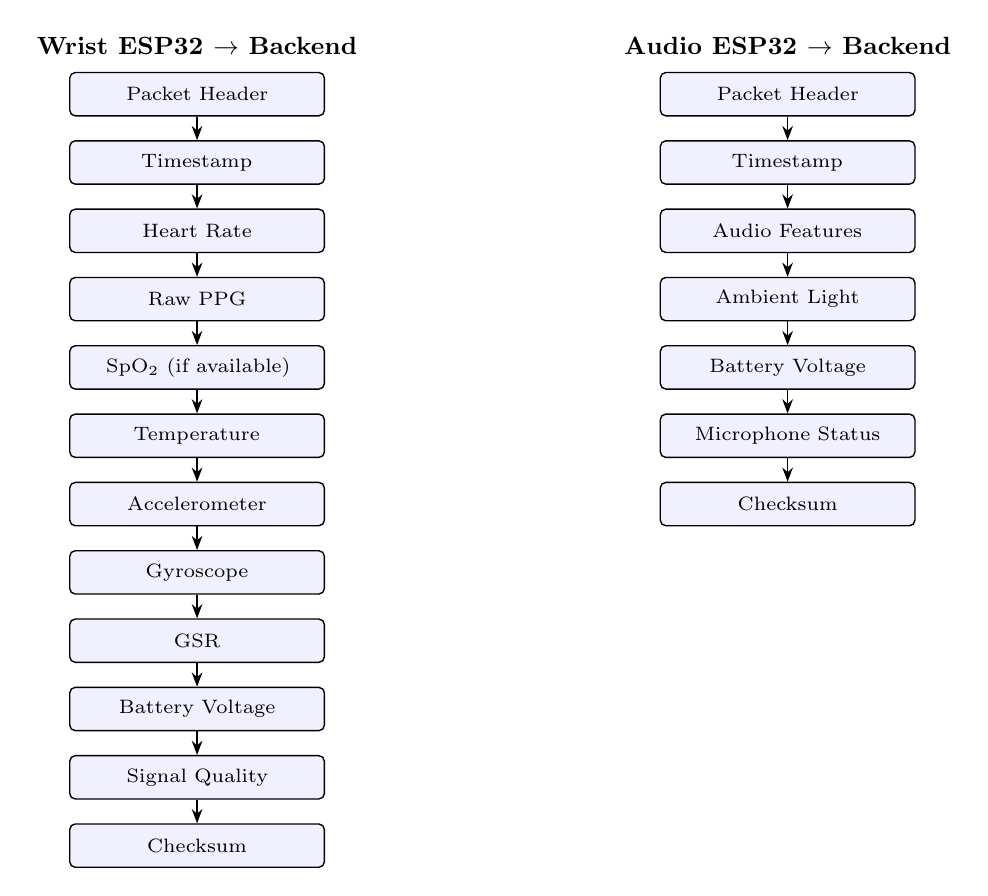
\begin{tikzpicture}[
    font=\scriptsize,
    field/.style={draw, rounded corners=2pt, text width=3.0cm, minimum height=0.55cm, align=center, line width=0.5pt, fill=blue!6},
    arrow/.style={-{Stealth[length=1.8mm]}, line width=0.5pt}
]
% Wrist packet (left column)
\node[field] (w1) at (0,7.5) {Packet Header};
\node[field, below=3mm of w1] (w2) {Timestamp};
\node[field, below=3mm of w2] (w3) {Heart Rate};
\node[field, below=3mm of w3] (w4) {Raw PPG};
\node[field, below=3mm of w4] (w5) {SpO\textsubscript{2} (if available)};
\node[field, below=3mm of w5] (w6) {Temperature};
\node[field, below=3mm of w6] (w7) {Accelerometer};
\node[field, below=3mm of w7] (w8) {Gyroscope};
\node[field, below=3mm of w8] (w9) {GSR};
\node[field, below=3mm of w9] (w10) {Battery Voltage};
\node[field, below=3mm of w10] (w11) {Signal Quality};
\node[field, below=3mm of w11] (w12) {Checksum};

\foreach \i/\j in {w1/w2, w2/w3, w3/w4, w4/w5, w5/w6, w6/w7, w7/w8, w8/w9, w9/w10, w10/w11, w11/w12}
  \draw[arrow] (\i.south) -- (\j.north);

\node[above=1mm of w1, font=\bfseries\small] {Wrist ESP32 $\to$ Backend};

% Audio packet (right column)
\node[field] (a1) at (7.5,7.5) {Packet Header};
\node[field, below=3mm of a1] (a2) {Timestamp};
\node[field, below=3mm of a2] (a3) {Audio Features};
\node[field, below=3mm of a3] (a4) {Ambient Light};
\node[field, below=3mm of a4] (a5) {Battery Voltage};
\node[field, below=3mm of a5] (a6) {Microphone Status};
\node[field, below=3mm of a6] (a7) {Checksum};

\foreach \i/\j in {a1/a2, a2/a3, a3/a4, a4/a5, a5/a6, a6/a7}
  \draw[arrow] (\i.south) -- (\j.north);

\node[above=1mm of a1, font=\bfseries\small] {Audio ESP32 $\to$ Backend};

\end{tikzpicture}
\caption{Field structure of packets transmitted from the Wrist ESP32 (left, 12 fields) and Audio ESP32 (right, 7 fields) to the backend.}
\label{fig:packet-structures}
\end{figure*}

\subsection{Synchronization}
\label{sec:comm-synchronization}

Both ESP32 modules should maintain synchronized timestamps. \Cref{fig:sync-sequence} shows the recommended synchronization sequence.

\begin{figure}[H]
\centering
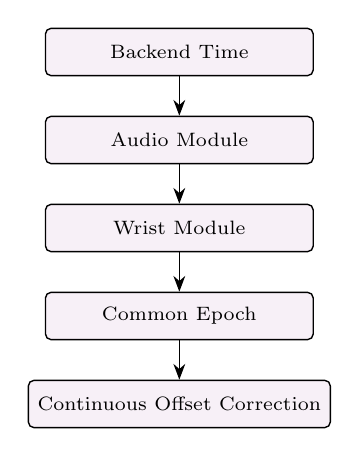
\begin{tikzpicture}[
    font=\scriptsize,
    node distance=0mm,
    field/.style={draw, rounded corners=2pt, fill=violet!6, minimum width=3.4cm, minimum height=0.6cm, align=center, line width=0.5pt}
]
\node[field] (s1) {Backend Time};
\node[field, below=5mm of s1] (s2) {Audio Module};
\node[field, below=5mm of s2] (s3) {Wrist Module};
\node[field, below=5mm of s3] (s4) {Common Epoch};
\node[field, below=5mm of s4] (s5) {Continuous Offset Correction};

\foreach \i/\j in {s1/s2, s2/s3, s3/s4, s4/s5}
  \draw[-{Stealth[length=2mm]}, line width=0.6pt] (\i.south) -- (\j.north);
\end{tikzpicture}
\caption{Recommended synchronization sequence, from backend time distribution through per-module alignment to a common epoch with continuous offset correction.}
\label{fig:sync-sequence}
\end{figure}


% ============================================================
% CHAPTER 26
% ============================================================
% ============================================================
% Chapter 26 — Firmware Architecture
% Source: PSYCON Engineering Design Document, Vol. 5, Ch. 26
% ============================================================
\section{Firmware Architecture}
\label{sec:firmware-architecture-ref}

\Cref{fig:firmware-boot-sequences} shows the boot-to-shutdown sequence for the Wrist and Audio firmware.

\begin{figure*}[t]
\centering
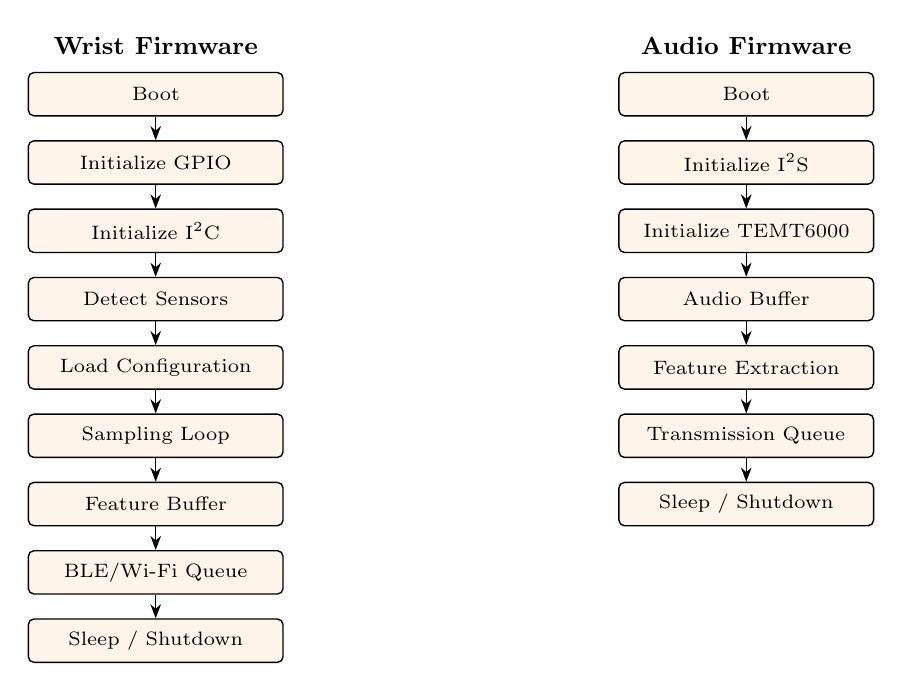
\begin{tikzpicture}[
    font=\scriptsize,
    field/.style={draw, rounded corners=2pt, text width=3.0cm, minimum height=0.55cm, align=center, line width=0.5pt, fill=orange!8},
    arrow/.style={-{Stealth[length=1.8mm]}, line width=0.5pt}
]
% Wrist firmware (left)
\node[field] (w1) at (0,6) {Boot};
\node[field, below=3mm of w1] (w2) {Initialize GPIO};
\node[field, below=3mm of w2] (w3) {Initialize I\textsuperscript{2}C};
\node[field, below=3mm of w3] (w4) {Detect Sensors};
\node[field, below=3mm of w4] (w5) {Load Configuration};
\node[field, below=3mm of w5] (w6) {Sampling Loop};
\node[field, below=3mm of w6] (w7) {Feature Buffer};
\node[field, below=3mm of w7] (w8) {BLE/Wi-Fi Queue};
\node[field, below=3mm of w8] (w9) {Sleep / Shutdown};

\foreach \i/\j in {w1/w2, w2/w3, w3/w4, w4/w5, w5/w6, w6/w7, w7/w8, w8/w9}
  \draw[arrow] (\i.south) -- (\j.north);

\node[above=1mm of w1, font=\bfseries\small] {Wrist Firmware};

% Audio firmware (right)
\node[field] (a1) at (7.5,6) {Boot};
\node[field, below=3mm of a1] (a2) {Initialize I\textsuperscript{2}S};
\node[field, below=3mm of a2] (a3) {Initialize TEMT6000};
\node[field, below=3mm of a3] (a4) {Audio Buffer};
\node[field, below=3mm of a4] (a5) {Feature Extraction};
\node[field, below=3mm of a5] (a6) {Transmission Queue};
\node[field, below=3mm of a6] (a7) {Sleep / Shutdown};

\foreach \i/\j in {a1/a2, a2/a3, a3/a4, a4/a5, a5/a6, a6/a7}
  \draw[arrow] (\i.south) -- (\j.north);

\node[above=1mm of a1, font=\bfseries\small] {Audio Firmware};

\end{tikzpicture}
\caption{Boot-to-shutdown sequence for the Wrist firmware (left, 9 stages) and Audio firmware (right, 7 stages).}
\label{fig:firmware-boot-sequences}
\end{figure*}

\subsection{Wrist Firmware Tasks}
\label{sec:wrist-firmware-tasks-ref}

\begin{itemize}
    \item Power management
    \item Sensor polling
    \item Timestamp generation
    \item Error logging
    \item Battery monitoring
    \item Packet transmission
    \item Watchdog servicing
\end{itemize}


% ============================================================
% CHAPTER 27
% ============================================================
% ============================================================
% Chapter 27 — Backend Software Architecture
% Source: PSYCON Engineering Design Document, Vol. 5, Ch. 27
% ============================================================
\section{Backend Software Architecture}
\label{sec:backend-software-architecture}

\Cref{fig:backend-architecture-ref} shows the end-to-end backend software pipeline. Modules should be independently testable and version-controlled.

\begin{figure*}[t]
\centering
\resizebox{\textwidth}{!}{%
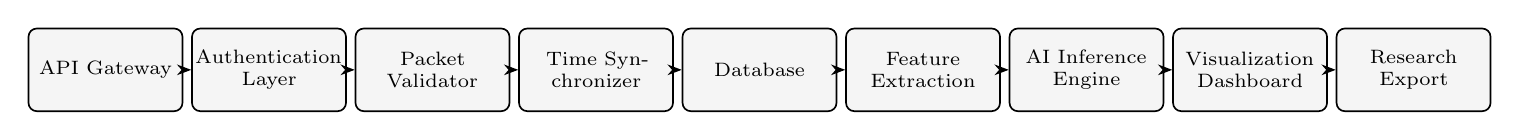
\begin{tikzpicture}[
    font=\scriptsize,
    stage/.style={draw, rounded corners=3pt, text width=1.85cm, minimum height=1.05cm, align=center, line width=0.6pt, fill=gray!8, inner sep=1.5pt},
    arrow/.style={-{Stealth[length=1.8mm]}, line width=0.5pt},
    node distance=1mm
]
\node[stage] (s1) {API Gateway};
\node[stage, right=of s1] (s2) {Authentication Layer};
\node[stage, right=of s2] (s3) {Packet Validator};
\node[stage, right=of s3] (s4) {Time Synchronizer};
\node[stage, right=of s4] (s5) {Database};
\node[stage, right=of s5] (s6) {Feature Extraction};
\node[stage, right=of s6] (s7) {AI Inference Engine};
\node[stage, right=of s7] (s8) {Visualization Dashboard};
\node[stage, right=of s8] (s9) {Research Export};

\foreach \i/\j in {s1/s2, s2/s3, s3/s4, s4/s5, s5/s6, s6/s7, s7/s8, s8/s9}
  \draw[arrow] (\i.east) -- (\j.west);
\end{tikzpicture}%
}
\caption{End-to-end backend software pipeline, from API gateway and authentication through packet validation, time synchronization, storage, feature extraction, AI inference, visualization, and research export.}
\label{fig:backend-architecture-ref}
\end{figure*}


% ============================================================
% CHAPTER 28
% ============================================================
% ============================================================
% Chapter 28 — Complete Test Procedures
% Source: PSYCON Engineering Design Document, Vol. 5, Ch. 28
% ============================================================
\section{Complete Test Procedures}
\label{sec:complete-test-procedures}

\Cref{tab:complete-test-procedures} consolidates the complete set of test procedures across hardware, electrical, firmware, AI, and mechanical domains.

\begin{table*}[t]
\centering
\caption{Complete test procedures by category.}
\label{tab:complete-test-procedures}
\small
\begin{tabularx}{\textwidth}{@{}l Y@{}}
\toprule
\textbf{Category} & \textbf{Test Items} \\
\midrule
Hardware & Visual inspection; connector inspection; battery polarity verification; sensor detection; charging verification; thermal inspection \\
Electrical & Supply voltage validation; brownout verification; current consumption; runtime testing; charging cycle testing \\
Firmware & Boot reliability; sensor initialization; error recovery; watchdog operation; memory stability; long-duration operation \\
AI & Dataset integrity; feature extraction validation; training reproducibility; cross-validation; performance evaluation; error analysis \\
Mechanical & Wearability; strap integrity; enclosure fit; cable strain relief; button accessibility; charging access \\
\bottomrule
\end{tabularx}
\end{table*}

\subsection{Week 6 execution and acceptance}

The detailed procedure, calibration methods, safety stops, measurement fields, and acceptance rules are maintained in \texttt{docs/validation/WEEK\_6\_RUNBOOK.md}. Evidence is evaluated with:

\begin{verbatim}
python -m validation.report
  --evidence <file.json>
  --output-dir validation-output/report
\end{verbatim}

The report returns a nonzero status while required evidence is missing or a stage is open. Software checks run through \texttt{python -m pytest tests/validation}; a running backend can additionally execute \texttt{validation.api\_validation} and \texttt{validation.stress}. Simulated results are useful for transport and failure handling but cannot substitute for the complete-system one-hour physical stress test or six-hour battery-powered test.

\begin{warningbox}
No charger or wired external power may be connected while the device is worn, and charging is prohibited whenever GSR electrodes are attached. Human GSR contact is prohibited until excitation, current limiting, insulation, and fault behavior pass electrical review on the exact hardware revision.
\end{warningbox}


% ============================================================
% CHAPTER 29
% ============================================================
% ============================================================
% Chapter 29 — Maintenance Schedule
% Source: PSYCON Engineering Design Document, Vol. 5, Ch. 29
% ============================================================
\section{Maintenance Schedule}
\label{sec:maintenance-schedule}

\Cref{tab:maintenance-schedule} lists recommended maintenance tasks by frequency.

\begin{table}[H]
\centering
\caption{Maintenance schedule by frequency.}
\label{tab:maintenance-schedule}
\small
\begin{tabularx}{\columnwidth}{@{}l Y@{}}
\toprule
\textbf{Frequency} & \textbf{Tasks} \\
\midrule
Before every use & Check battery charge; inspect wiring; clean optical sensor; clean GSR electrodes; verify microphone opening \\
Weekly & Inspect solder joints; verify charging; check firmware version; review logs \\
Monthly & Recalibrate sensors (if applicable); battery health review; enclosure inspection; connector inspection \\
\bottomrule
\end{tabularx}
\end{table}

The Week 7 assembly and maintenance guide adds revision checks, cleaning, log review, backup restoration, access and retention review, battery retirement, storage, transport, and change control. Any wiring, power, charger, battery, sensor, connector, enclosure, acquisition, timing, buffering, communication, or recovery change creates a new affected revision and invalidates downstream calibration, runtime, and safety evidence until retested.


% ============================================================
% CHAPTER 30
% ============================================================
% ============================================================
% Chapter 30 — Troubleshooting Guide
% Source: PSYCON Engineering Design Document, Vol. 5, Ch. 30
% ============================================================
\section{Troubleshooting Guide}
\label{sec:troubleshooting-guide}

\Cref{tab:troubleshooting-guide} lists common symptoms, together with the possible causes or checks to perform.

\begin{table*}[t]
\centering
\caption{Troubleshooting guide: symptoms and possible causes or checks.}
\label{tab:troubleshooting-guide}
\small
\begin{tabularx}{\textwidth}{@{}l Y@{}}
\toprule
\textbf{Symptom} & \textbf{Possible Causes / Checks} \\
\midrule
Device does not boot & Battery discharged; incorrect polarity; loose connector; faulty regulator; firmware corruption \\
Sensor not detected & SDA; SCL; pull-ups; address conflicts; power supply; ground continuity \\
No audio & I\textsuperscript{2}S wiring; pin assignments; gain settings; DMA configuration; buffer overflow \\
Poor GSR signal & Electrode contact; motion artifacts; wiring; ADC configuration; analog front end \\
Random ESP32 reset & Brownout; insufficient power; memory exhaustion; watchdog timeout; software crash \\
\bottomrule
\end{tabularx}
\end{table*}


% ============================================================
% CHAPTER 31
% ============================================================
% ============================================================
% Chapter 31 — Glossary
% Source: PSYCON Engineering Design Document, Vol. 5, Ch. 31
% ============================================================
\section{Glossary}
\label{sec:glossary}

\Cref{tab:glossary} defines the abbreviations and terms used throughout this document.

\begin{table*}[t]
\centering
\caption{Glossary of terms and abbreviations.}
\label{tab:glossary}
\small
\begin{tabularx}{\textwidth}{@{}l Y@{}}
\toprule
\textbf{Term} & \textbf{Definition} \\
\midrule
ADC & Analog-to-Digital Converter \\
BLE & Bluetooth Low Energy \\
DMA & Direct Memory Access \\
EDA/GSR & Electrodermal Activity / Galvanic Skin Response \\
ESP32 & Dual-core Wi-Fi/Bluetooth microcontroller \\
HRV & Heart Rate Variability \\
I\textsuperscript{2}C & Inter-Integrated Circuit communication bus \\
I\textsuperscript{2}S & Integrated Interchip Sound interface \\
IMU & Inertial Measurement Unit \\
LiPo & Lithium Polymer battery \\
MCU & Microcontroller Unit \\
MFCC & Mel-Frequency Cepstral Coefficients \\
PCB & Printed Circuit Board \\
PPG & Photoplethysmography \\
SpO\textsubscript{2} & Peripheral oxygen saturation \\
UART & Universal Asynchronous Receiver Transmitter \\
\bottomrule
\end{tabularx}
\end{table*}


% ============================================================
% CHAPTER 32
% ============================================================
% ============================================================
% Chapter 32 — Revision History
% Source: PSYCON Engineering Design Document, Vol. 5, Ch. 32
% ============================================================
\section{Revision History}
\label{sec:revision-history}

\Cref{tab:revision-history} lists the document revision history.

\begin{table}[H]
\centering
\caption{Document revision history.}
\label{tab:revision-history}
\small
\begin{tabularx}{\columnwidth}{@{}l Y@{}}
\toprule
\textbf{Version} & \textbf{Description} \\
\midrule
v0.1 & Initial concept \\
v0.2 & Hardware selection \\
v0.3 & Sensor integration plan \\
v0.4 & Firmware architecture \\
v0.5 & AI pipeline definition \\
v0.6 & Validation strategy \\
v0.7 & Mechanical design \\
v0.8 & Competition documentation \\
v0.9 & Prototype integration \\
v1.0 & First complete engineering release \\
\bottomrule
\end{tabularx}
\end{table}


% ============================================================
% CHAPTER 33
% ============================================================
% ============================================================
% Chapter 33 — Final Project Checklist
% Source: PSYCON Engineering Design Document, Vol. 5, Ch. 33
% ============================================================
\section{Final Project Checklist}
\label{sec:final-project-checklist}

\subsection{Hardware}
\label{sec:checklist-hardware}

\begin{donelist}
    \item Component selection finalized
    \item Power architecture defined
    \item Sensor interfaces defined
    \item GPIO allocation documented
    \item I\textsuperscript{2}C address map documented
\end{donelist}
\begin{checklist}
    \item Final integrated assembly
    \item Electrical validation
    \item Runtime testing
\end{checklist}

\subsection{Firmware}
\label{sec:checklist-firmware}

\begin{donelist}
    \item Architecture defined
    \item Communication protocol defined
\end{donelist}
\begin{checklist}
    \item Complete implementation
    \item End-to-end testing
    \item Performance optimization
\end{checklist}

\subsection{AI}
\label{sec:checklist-ai}

\begin{donelist}
    \item Pipeline defined
    \item Feature plan documented
    \item Anonymous session metadata validation implemented
    \item Synchronized multimodal dataset assembly implemented
    \item Participant-separated model comparison implemented
    \item Consent, data handoff, and model lifecycle documented
\end{donelist}
\begin{checklist}
    \item Dataset collection
    \item Psychologist target definition and marksheet import
    \item Model training
    \item Multimodal ablation and duration results
    \item External validation
\end{checklist}

\subsection{Documentation}
\label{sec:checklist-documentation}

\begin{donelist}
    \item System architecture
    \item Bill of Materials (BOM)
    \item Wiring plan
    \item Risk assessment
    \item Research methodology
    \item Ethics documentation
    \item Maintenance plan
    \item Troubleshooting guide
    \item Reference index
    \item Competition documentation
\end{donelist}


% ============================================================
% CHAPTER 34
% ============================================================
% ============================================================
% Chapter 34 — Conclusion
% Source: PSYCON Engineering Design Document, Vol. 5, Ch. 34
% ============================================================
\section{Conclusion}
\label{sec:conclusion}

PSYCON is a modular research platform designed to investigate whether physiological measurements and speech-derived features can be combined to estimate indicators relevant to psychological well-being. Its split wearable architecture, documented hardware stack, and planned AI pipeline provide a structured foundation for research and engineering development.

The Week 7 repository can produce an integrity-checked software and documentation release candidate with operating, assembly, competition, AI, evidence, and demonstration instructions. It cannot produce a final competition release yet. The remaining work is real Wrist acquisition, a frozen physical build, electrical and battery evidence, GSR approval, the five physical integration stages, an approved PSYCON dataset, model and external validation, third-person reproduction, and live and recorded demonstrations.

\begin{warningbox}
Throughout development and presentation, the system should be described as a research and screening prototype, not as a medical diagnostic device.
\end{warningbox}


\printbibliography

\end{document}
